\documentclass{beamer}
\addtobeamertemplate{navigation symbols}{}{%
\usebeamerfont{footline}%
\usebeamercolor[fg]{footline}%
\hspace{5em}%
\large\insertframenumber
}
\setbeamercolor{footline}{fg=blue}
%\usetheme{Warsaw}

\usepackage[english, russian]{babel}
\usepackage[absolute,overlay]{textpos}
\usepackage{graphicx}
\usepackage{adjustbox}

\usefonttheme{professionalfonts}
\usepackage{fontspec}
\setmainfont{Times New Roman}
\setsansfont{Times New Roman}
\setmonofont{Consolas}
\renewcommand\fbox{\fcolorbox{blue}{white}}

\usepackage{array}
\usepackage{tcolorbox}
\usepackage{amsmath}
\usepackage{tikz}
\usepackage{blkarray}
\usepackage{listings}
\lstset{basicstyle=\footnotesize\ttfamily}
\lstset{escapeinside={<@}{@>}}
\usepackage[cache=false]{minted}
\newminted{python}{fontsize=\scriptsize, linenos=false}

\graphicspath{{../images/}}

\newcolumntype{C}[1]{>{\centering\arraybackslash}m{#1}}
\newcolumntype{L}[1]{>{\raggedright\arraybackslash}m{#1}}

\title{Моделирование перераспределения потоков между трещинами гидроразрыва пласта}
\subtitle{}
\author{Выполнил студент: А.~А.~Муравцев\and \\Научный руководитель: С.~А.~Калинин\and \\Консультант: И.~Ш.~Базыров}
\date{19 июня 2023 г.}

%\institute{
%\inst{1}
%Высшая школа теоретической механики и математической физики\\
%Санкт-Петербургский Политехнический университет Петра Великого
%}

\definecolor{new_green}{rgb}{0.20,0.68,0}
\definecolor{lit_gray}{cmyk}{0.7, 0.7, 0, 0}



\begin{document}


\begin{frame}
\vspace*{20mm}
\titlepage

\begin{textblock*}{128mm}(0cm,0.2cm)
\begin{center}
Санкт-Петербургский политехнический	университет Петра Великого\\
Физико-Механический институт\\
Высшая школа теоретической механики и математической физики
\end{center}
\end{textblock*}

\end{frame}


\begin{frame}
\frametitle{Проблематика и актуальность работы}

\begin{textblock*}{10.5cm}(0.5cm,1.3cm)
\begin{itemize}
	\item при эксплуатации месторождения во время перевода скважин с проведённым многостадийным гидроразрывом пласта в нагнетание (с целью поддержания пластового давления) практически невозможно избежать роста нескольких трещин автоГРП
	%\item при прорыве трещин автоГРП к добывающим скважинам существенно снижаются площадь охвата заводнением и эффективность эксплуатации месторождения
	\item важно научиться моделировать одновременный рост нескольких трещин автоГРП и перераспределение потоков между ними, чтобы не допускать снижения эффективности эксплуатации месторождения вследствие прорыва трещин автоГРП к добывающим скважинам 
\end{itemize}
\end{textblock*}

\begin{textblock*}{4.5cm}(1.5cm,6.5cm)
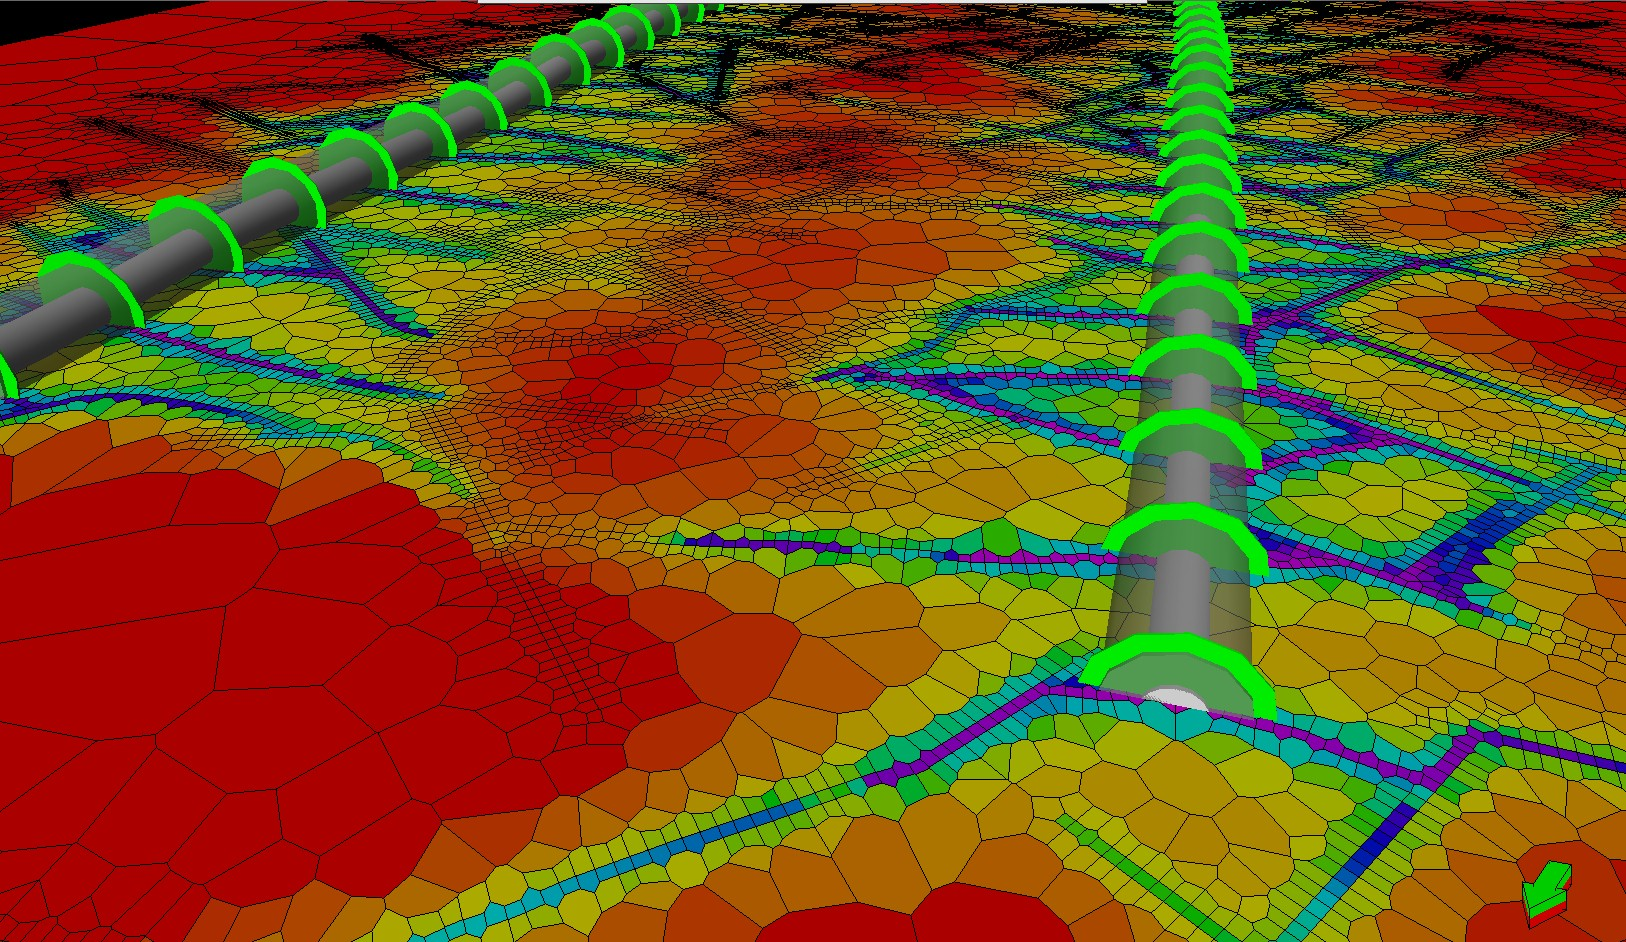
\includegraphics[width=4.5cm]{hydraulic_fracturing_abstract_image1.jpeg}
\end{textblock*}

\begin{textblock*}{4cm}(7.7cm,6.1cm)
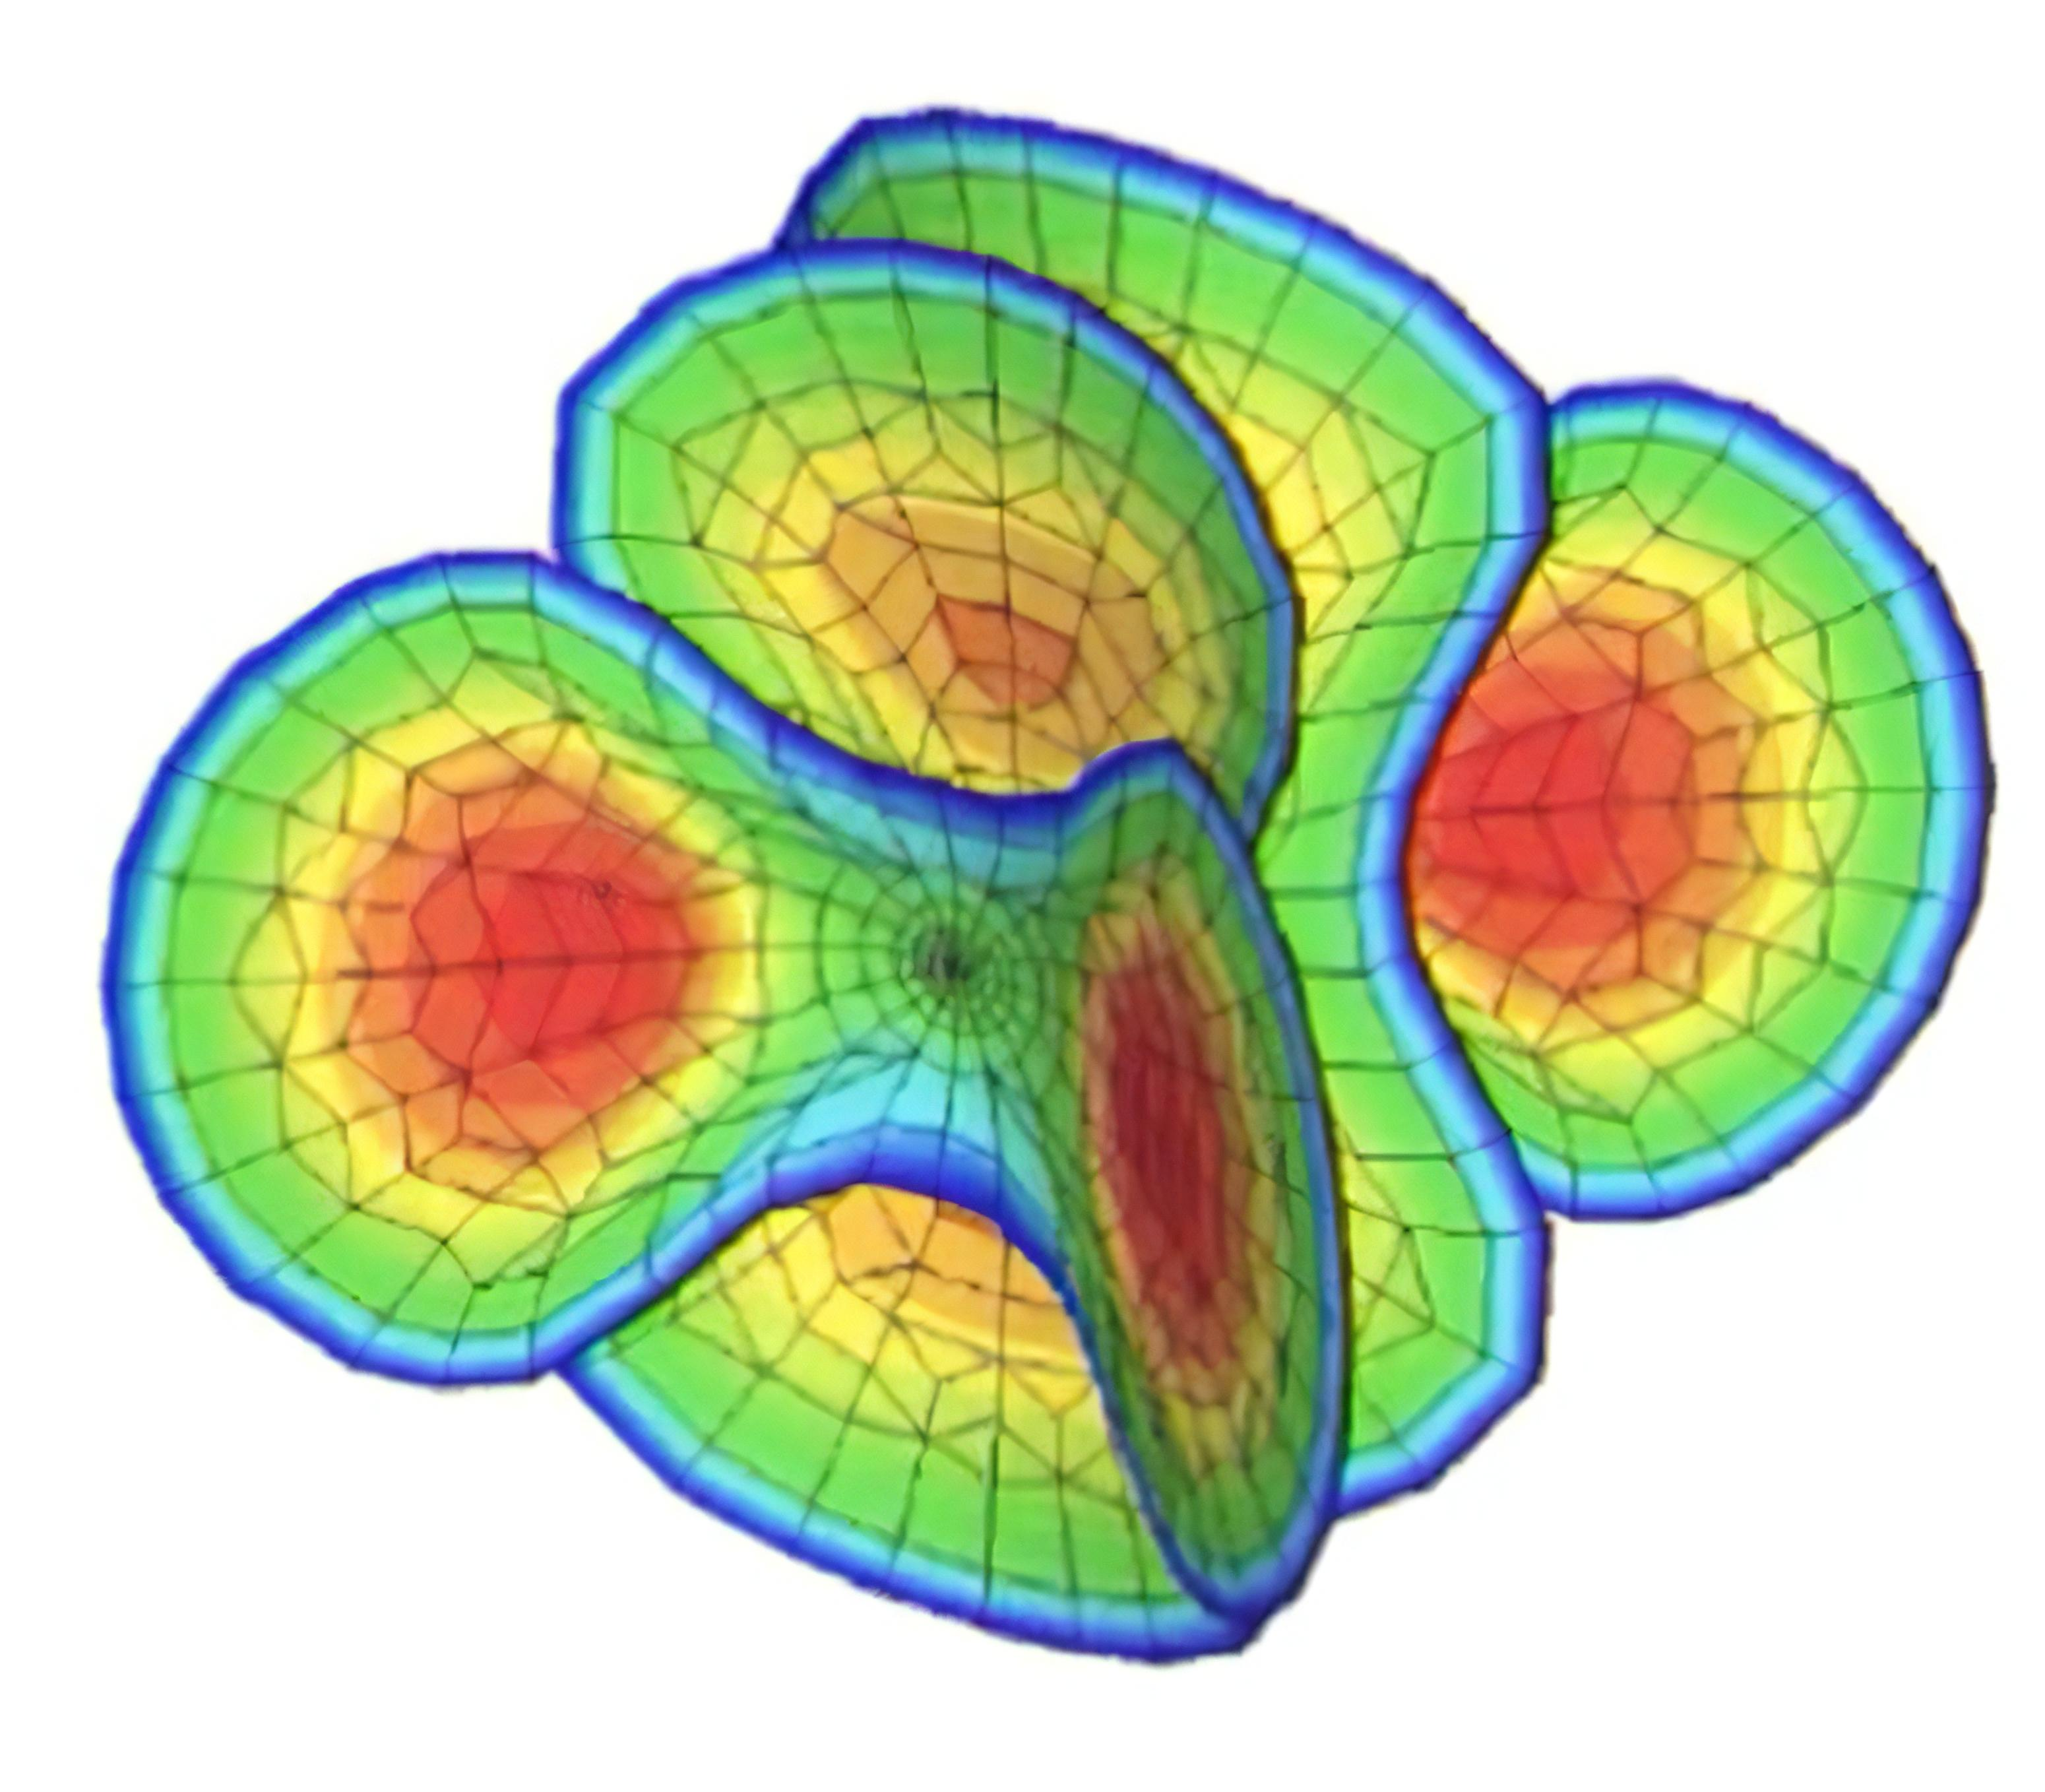
\includegraphics[width=3cm]{hydraulic_fracturing_abstract_image2.jpg}
\end{textblock*}

\end{frame}


\begin{frame}
\frametitle{Цель и задачи работы}

\textbf{Цель:}
\begin{itemize}
	\item построить модель совместного роста нескольких трещин автоГРП с учётом перераспределения потоков между ними
\end{itemize}

\textbf{Задачи:}
\begin{itemize}
	\item провести обзор имеющихся моделей роста трещины гидроразрыва пласта и выбрать наиболее подходящую модель для роста трещины автоГРП
	\item построить физико-математическую модель роста нескольких трещин автоГРП
	\item реализовать численный алгоритм решения на Python
	\item построить графики зависимостей полудлины каждой из трещин автоГРП и расходов на каждой из трещин от времени
	\item построить график зависимости забойного давления от времени
\end{itemize}

\end{frame}


\begin{frame}
\frametitle{Основные компоненты полной модели трещины ГРП}

\begin{textblock*}{8.8cm}(0.5cm,1.1cm)
\begin{enumerate}[1)]
	\item закон сохранения жидкости (доминирование или отсутствие утечек);
	\item уравнение течения жидкости в трещине (в зависимости от реологии жидкости);
	\item уравнение упругости для горной породы;
	\item условие распространения трещины;
	\item транспорт проппанта
\end{enumerate}
\end{textblock*}

\begin{textblock*}{3cm}(9.3cm,1.2cm)
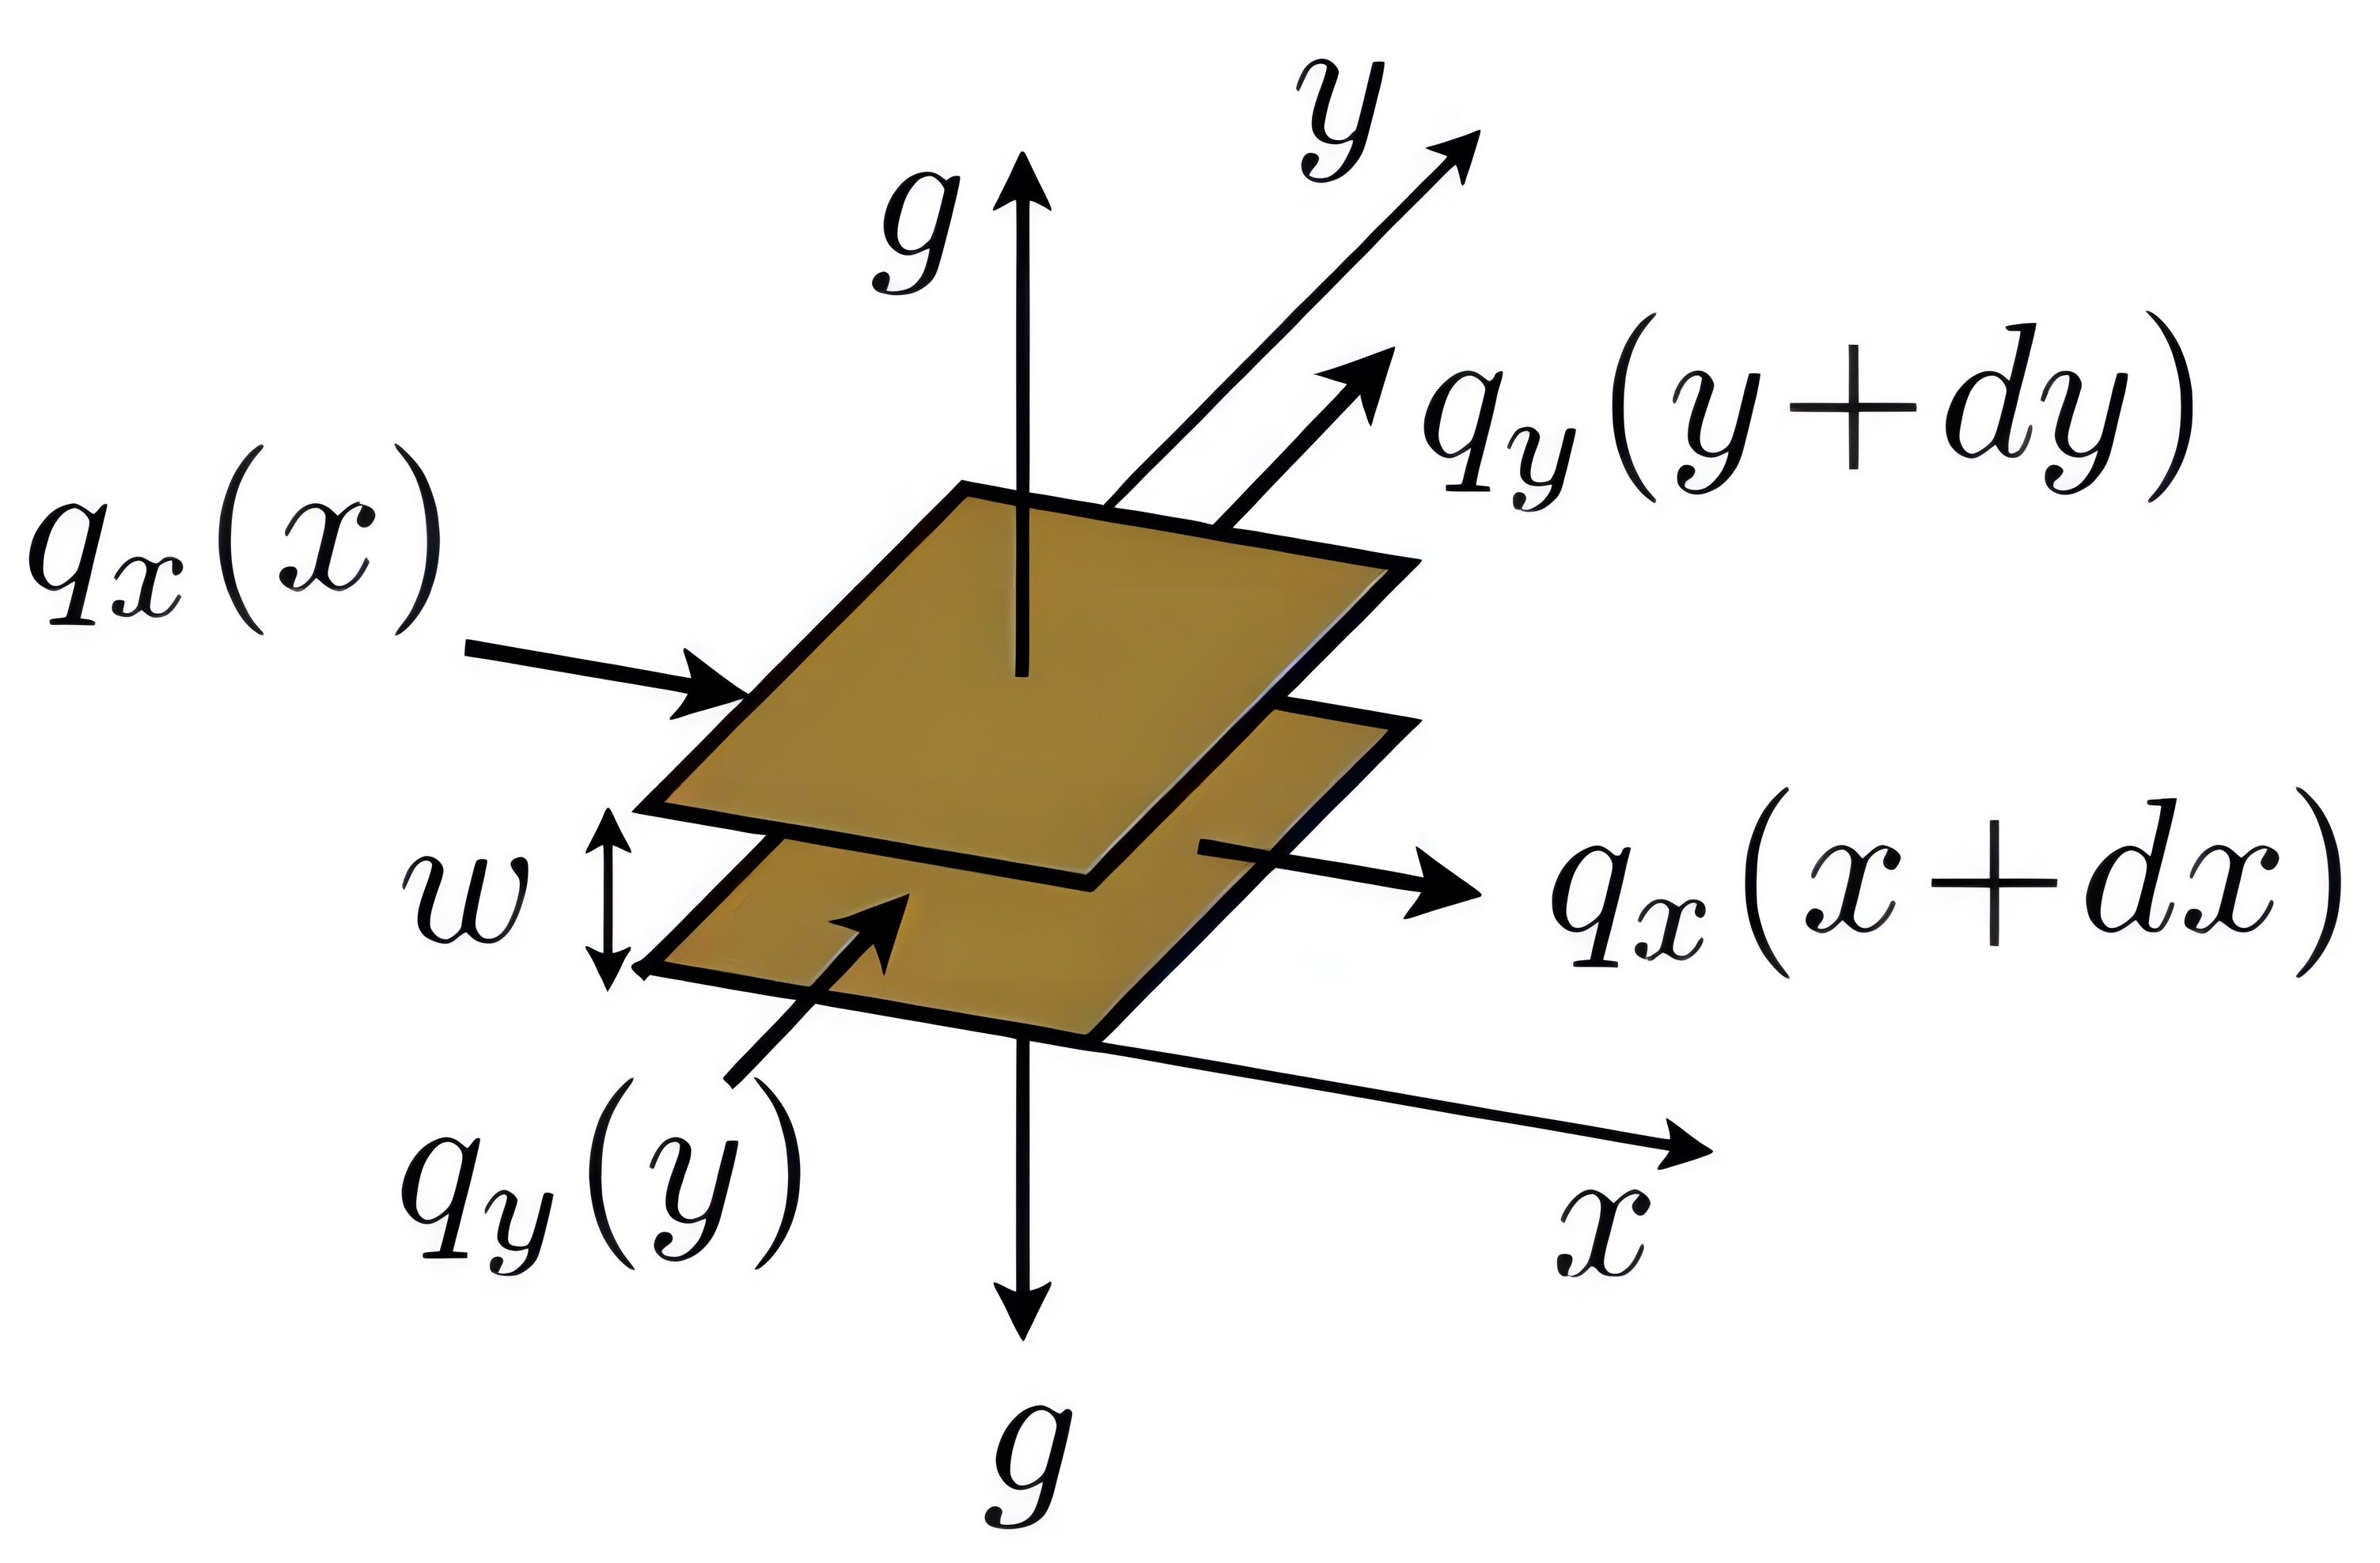
\includegraphics[width=3cm]{part1_balance.jpg}
\end{textblock*}

\begin{textblock*}{4cm}(0.7cm,5.2cm)
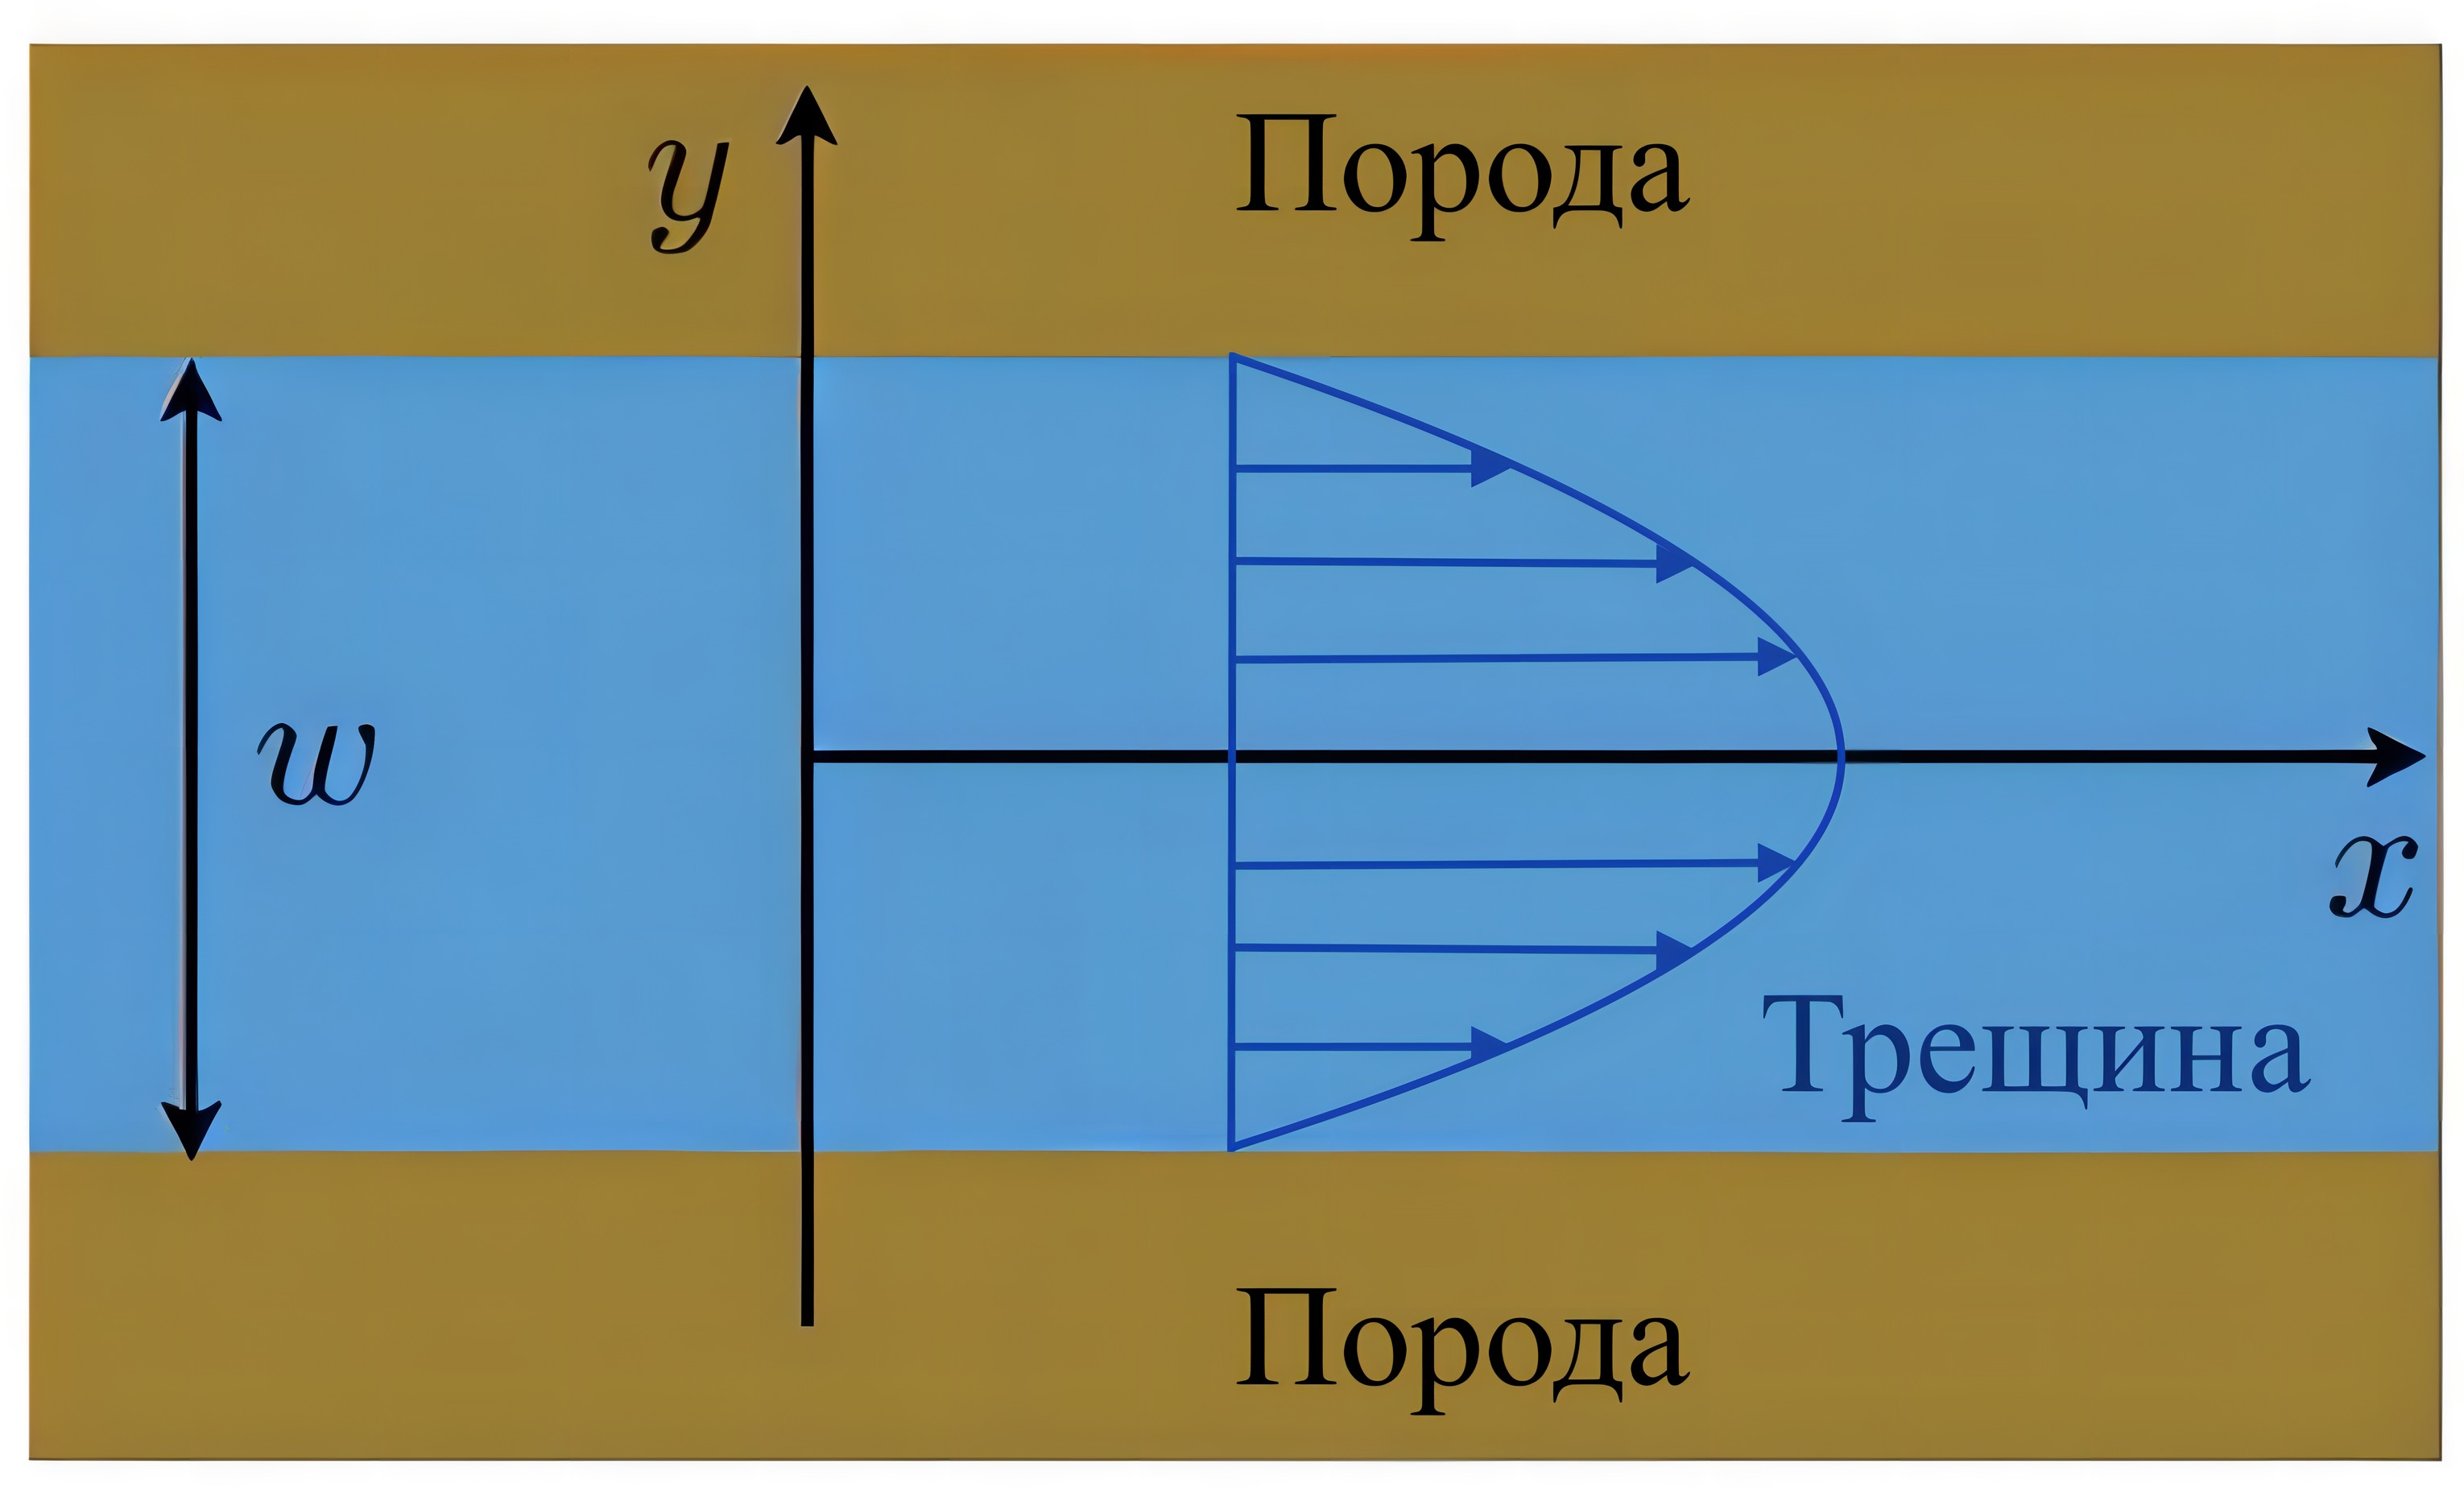
\includegraphics[width=4cm]{part2_flux.jpg}
\end{textblock*}

\begin{textblock*}{3.5cm}(8.5cm,3.2cm)
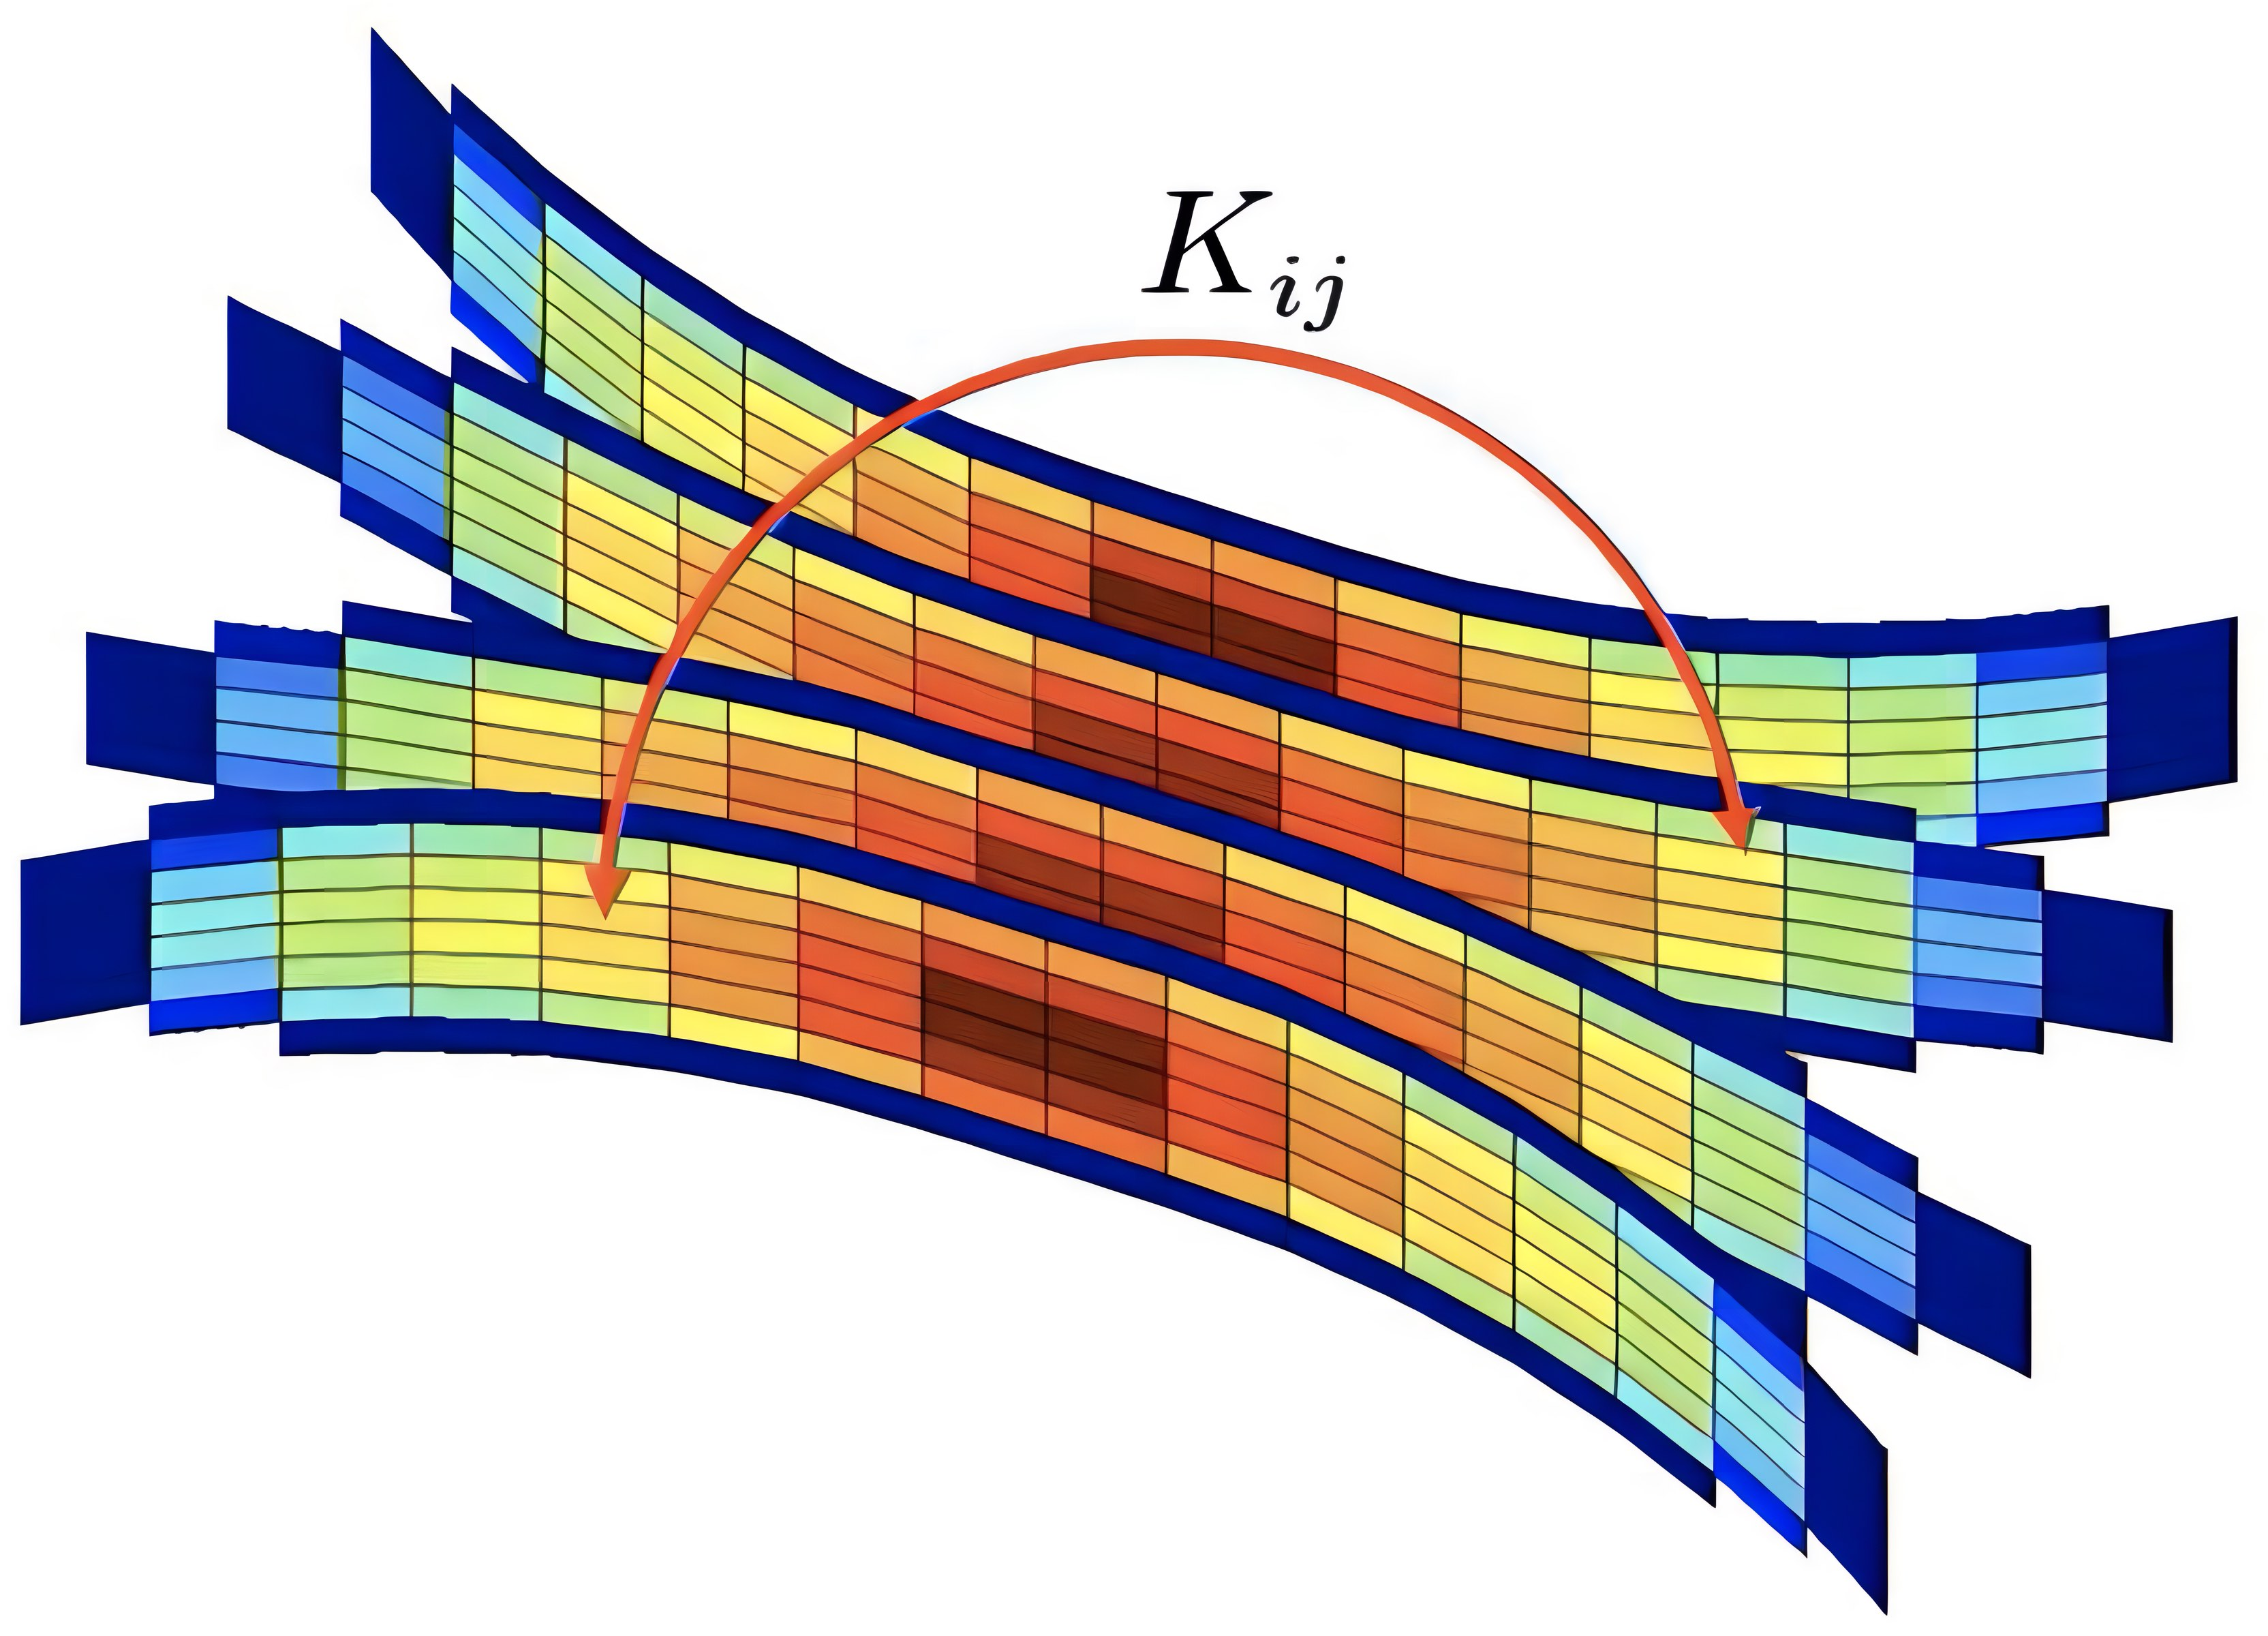
\includegraphics[width=3.5cm]{part3_elasticity.jpg}
\end{textblock*}


\begin{textblock*}{3cm}(5.5cm,4.5cm)
\tiny
$$
w=\sqrt{\frac{32}{\pi}}\frac{K_{I}\left(1-\nu^2\right)}{E}\sqrt{r}
$$
\normalsize
\end{textblock*}

\begin{textblock*}{7.5cm}(5cm,5.8cm)
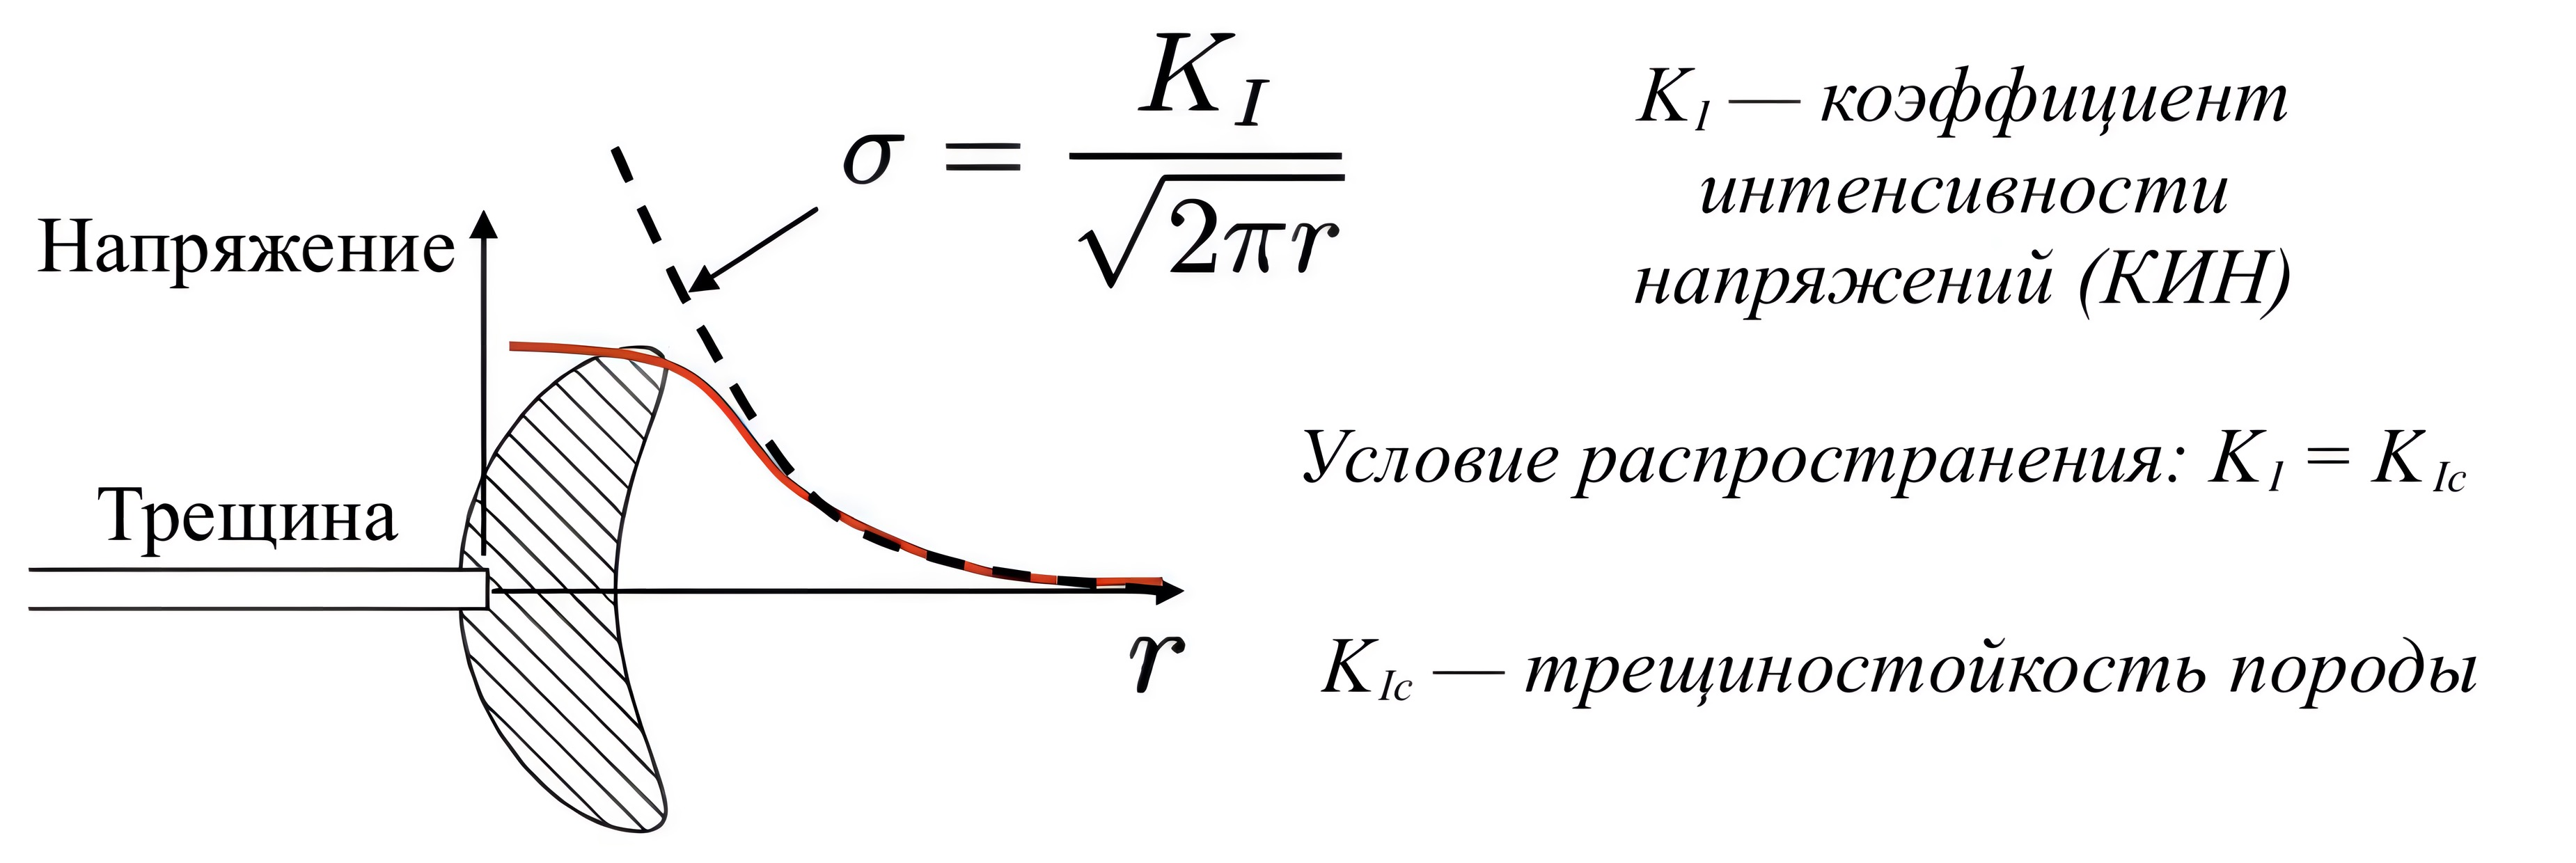
\includegraphics[width=7.5cm]{part4_propagation.jpg}
\end{textblock*}

\begin{textblock*}{6cm}(0.5cm,8.5cm)
\tiny
\textcolor{lit_gray}{A.V. Valov, A.N. Baykin, E.V. Dontsov.  Modeling geometry of planar hydraulic fractures using the Planar 3D ILSA approach}

\end{textblock*}

\begin{textblock*}{6cm}(7cm,8.5cm)
\tiny
\textcolor{lit_gray}{J.R. Rice. Mathematical analysis in the mechanics of fracture. Fracture: an advanced treatise, vol. II, pp. 191-311, 1968}
\end{textblock*}

\end{frame}

\begin{comment}
\begin{frame}
\frametitle{Модель Христиановича-Желтова-Гиртсма-деКлерка (модель плоской трещины)}

\footnotesize

\begin{textblock*}{6cm}(0.5cm,1.7cm)
$$
\begin{cases}
\dfrac{\partial w}{\partial t}+\dfrac{\partial q}{\partial x}+\dfrac{C'}{\sqrt{t-t_0(x)}}=Q_0(t)\delta(x),\\[15pt]
q=-\dfrac{w^3}{\mu'}\dfrac{\partial p}{\partial x},\\[5pt]
p(x,t)=\sigma_0-\dfrac{E'}{4\pi}\displaystyle\int\limits_{-L(t)}^{L(t)}\dfrac{w(s)ds}{(x-s)^2},\\[20pt]
\displaystyle\lim_{x\to L}\dfrac{w}{(L-x)^{1/2}}=\dfrac{K'}{E'},
\end{cases}
$$
где $C'=2C_l$; $\,\,\,\mu'=12\mu$; $\,\,\,E'=\dfrac{E}{1-\nu^2}$; $\,\,\,K'=\dfrac{8K_{Ic}}{\sqrt{2\pi}}$.
\end{textblock*}

\begin{textblock*}{8cm}(6.5cm,1.1cm)
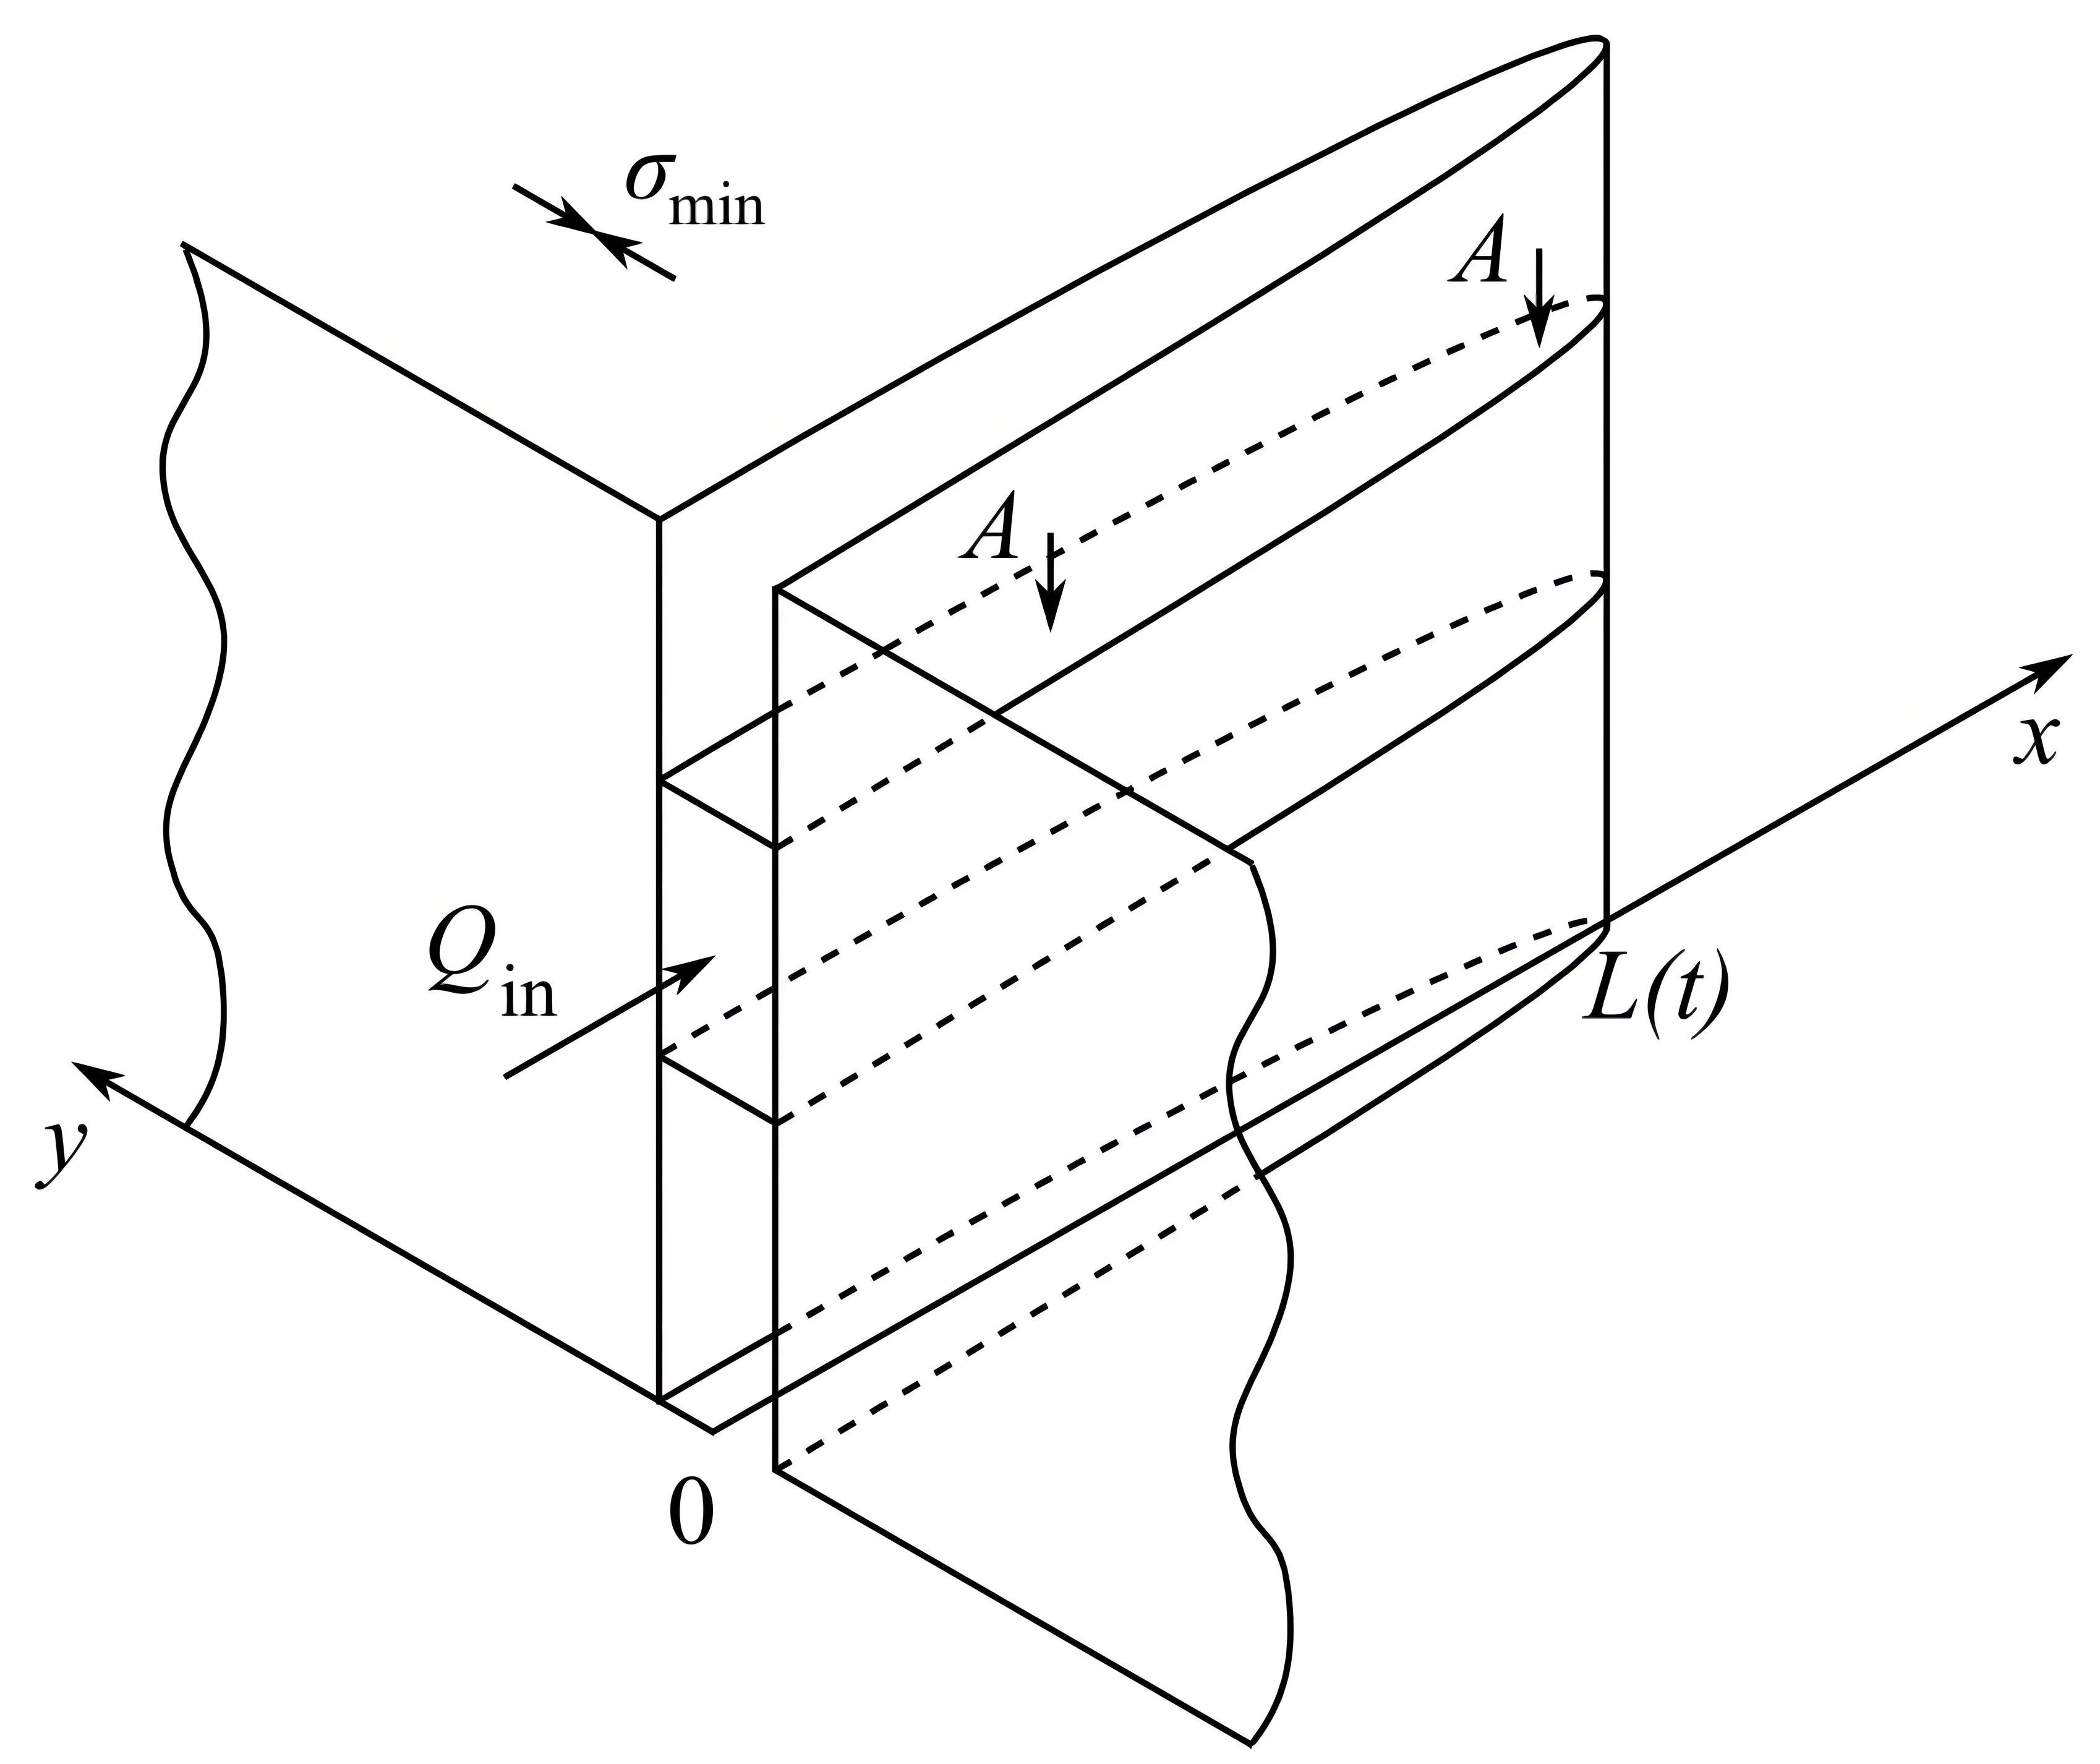
\includegraphics[width=6cm]{kgd_model_3D.jpg}
\end{textblock*}

\begin{textblock*}{8cm}(6.5cm,6.1cm)
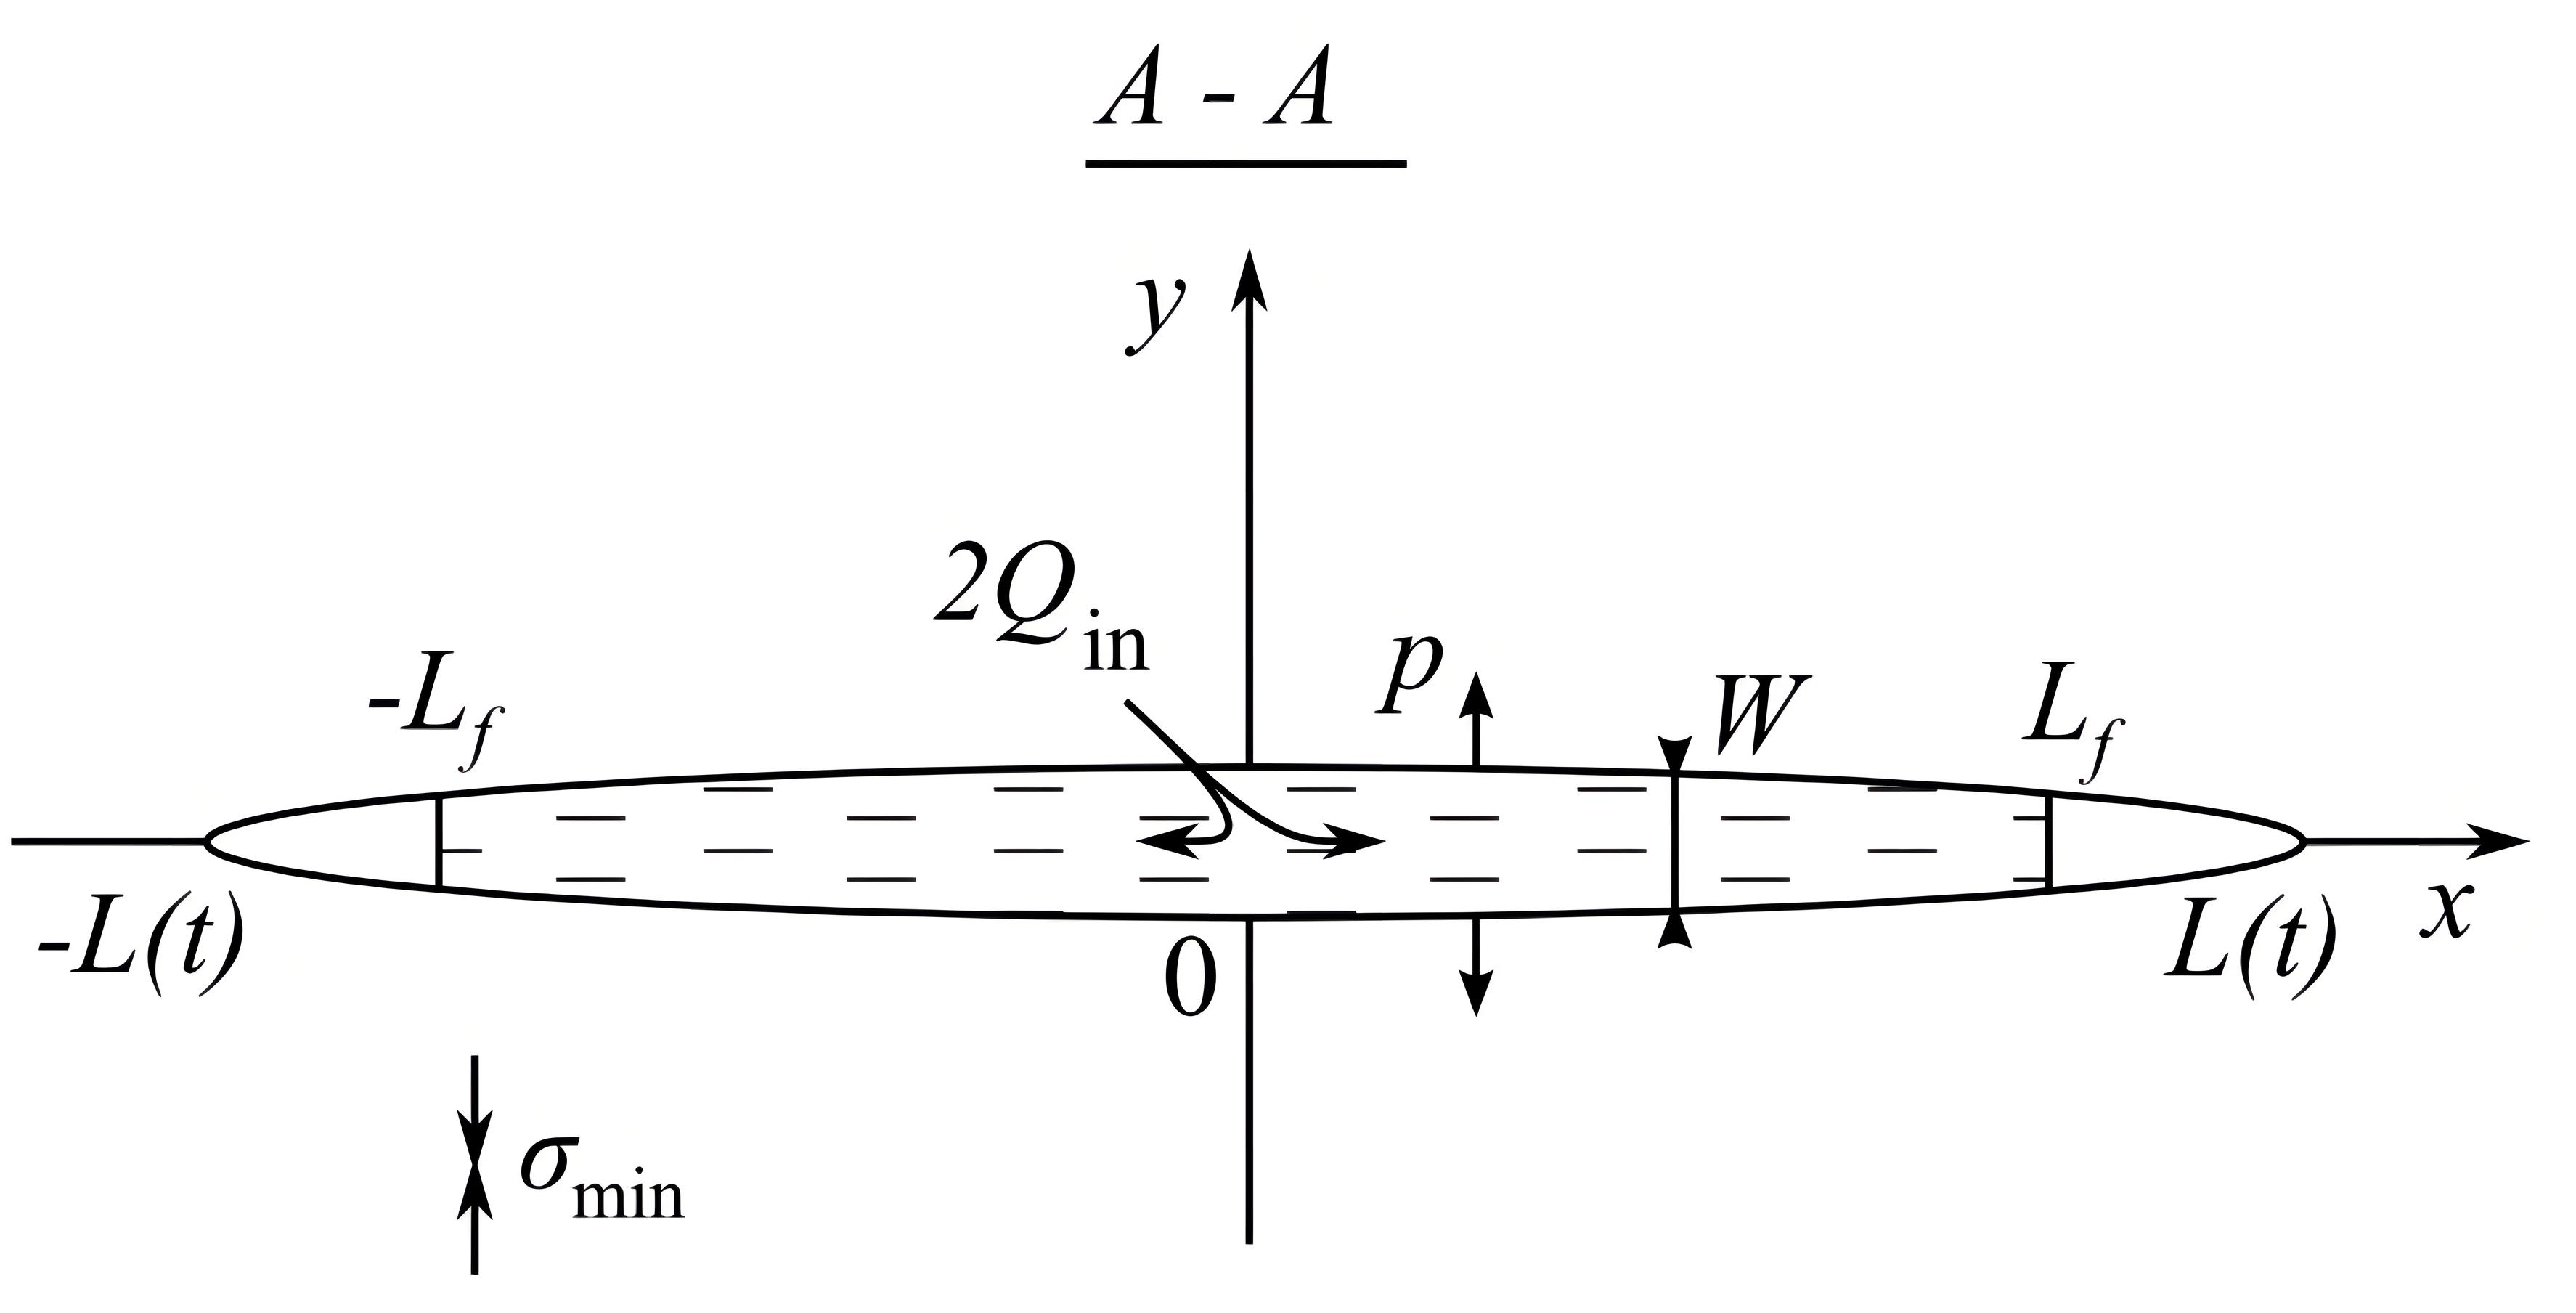
\includegraphics[width=6cm]{kgd_model_A-A_plane.jpg}
\end{textblock*}

\begin{textblock*}{6cm}(0.5cm,8.7cm)
\tiny
\textcolor{lit_gray}{E.V. Dontsov. An approximate solution for a plane strain hydraulic fracture that accounts for fracture toughness, fluid viscosity, and leak-off. \emph{Int. J. Fract.}, 205:221-237, 2017}
\end{textblock*}

\normalsize

\end{frame}
\end{comment}

\begin{comment}
\begin{frame}
\frametitle{Модель радиальной трещины}

\scriptsize

\begin{textblock*}{7cm}(0.5cm,0.8cm)
$$
\begin{cases}
\dfrac{\partial w}{\partial t}+\dfrac{1}{r}\dfrac{\partial}{\partial r}\!\left(rq\right)+\dfrac{C'}{\sqrt{t-t_0(r)}}=Q_0\delta(r),\\[15pt]
q=-\dfrac{w^3}{\mu'}\dfrac{\partial p_n}{\partial r},\\[5pt]
p_n(r,t)=-\dfrac{E'}{2\pi R}\displaystyle\int\limits_{0}^{R(t)}M\!\left(\dfrac{r}{R},\dfrac{r'}{R}\right)\dfrac{\partial w(r',t)}{\partial r'}dr',\\[20pt]
\displaystyle\lim_{r\to R}\dfrac{w}{(R-r)^{1/2}}=\dfrac{K'}{E'},
\end{cases}
$$
где $C'=2C_l$; $\,\,\,\mu'=12\mu$; $\,\,\,E'=\dfrac{E}{1-\nu^2}$; $\,\,\,K'=\dfrac{8K_{Ic}}{\sqrt{2\pi}}$;
$$
M(\rho,s)=
\begin{cases}
\dfrac{1}{\rho}\,K\!\left(\dfrac{s^2}{\rho^2}\right)+\dfrac{\rho}{s^2-\rho^2}\,E\!\left(\dfrac{s^2}{\rho^2}\right)\\\ \\
\dfrac{s}{s^2-\rho^2}\,E\!\left(\dfrac{\rho^2}{s^2}\right)
\end{cases}
$$
\end{textblock*}

\begin{textblock*}{7cm}(7cm,1cm)
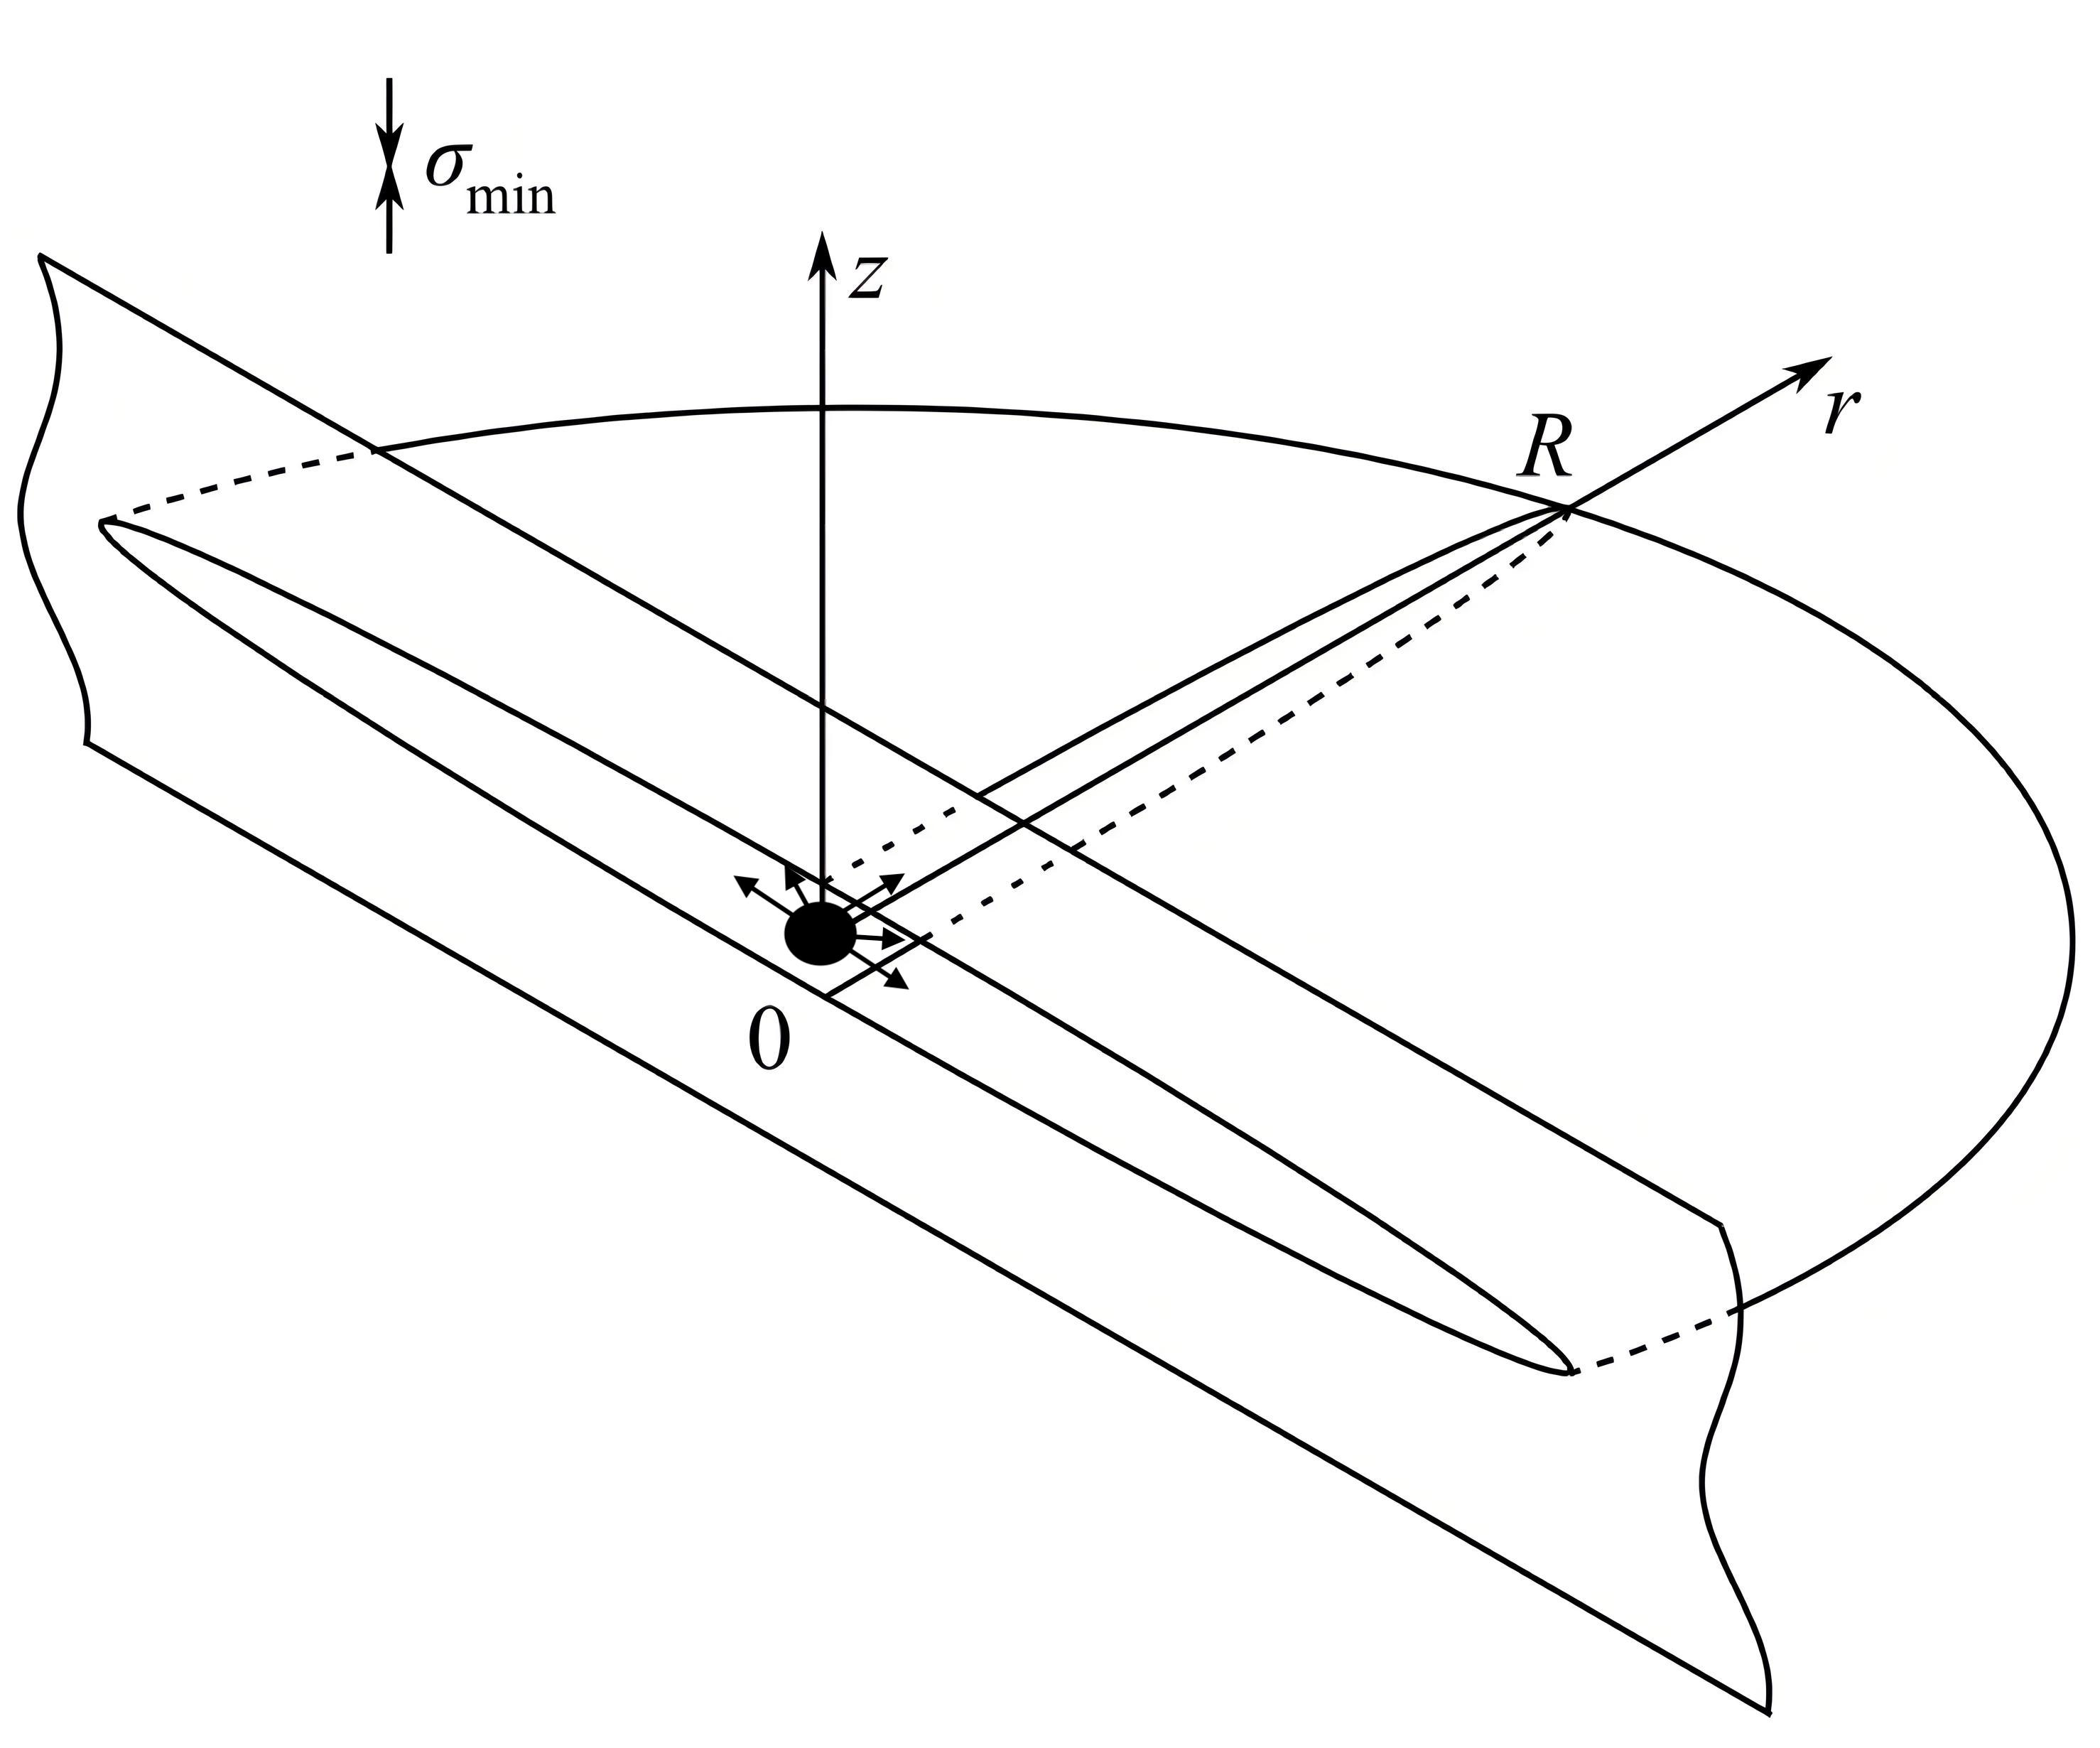
\includegraphics[width=5.5cm]{radial_model_3D.jpg}
\end{textblock*}

\begin{textblock*}{7cm}(7.4cm,5.7cm)
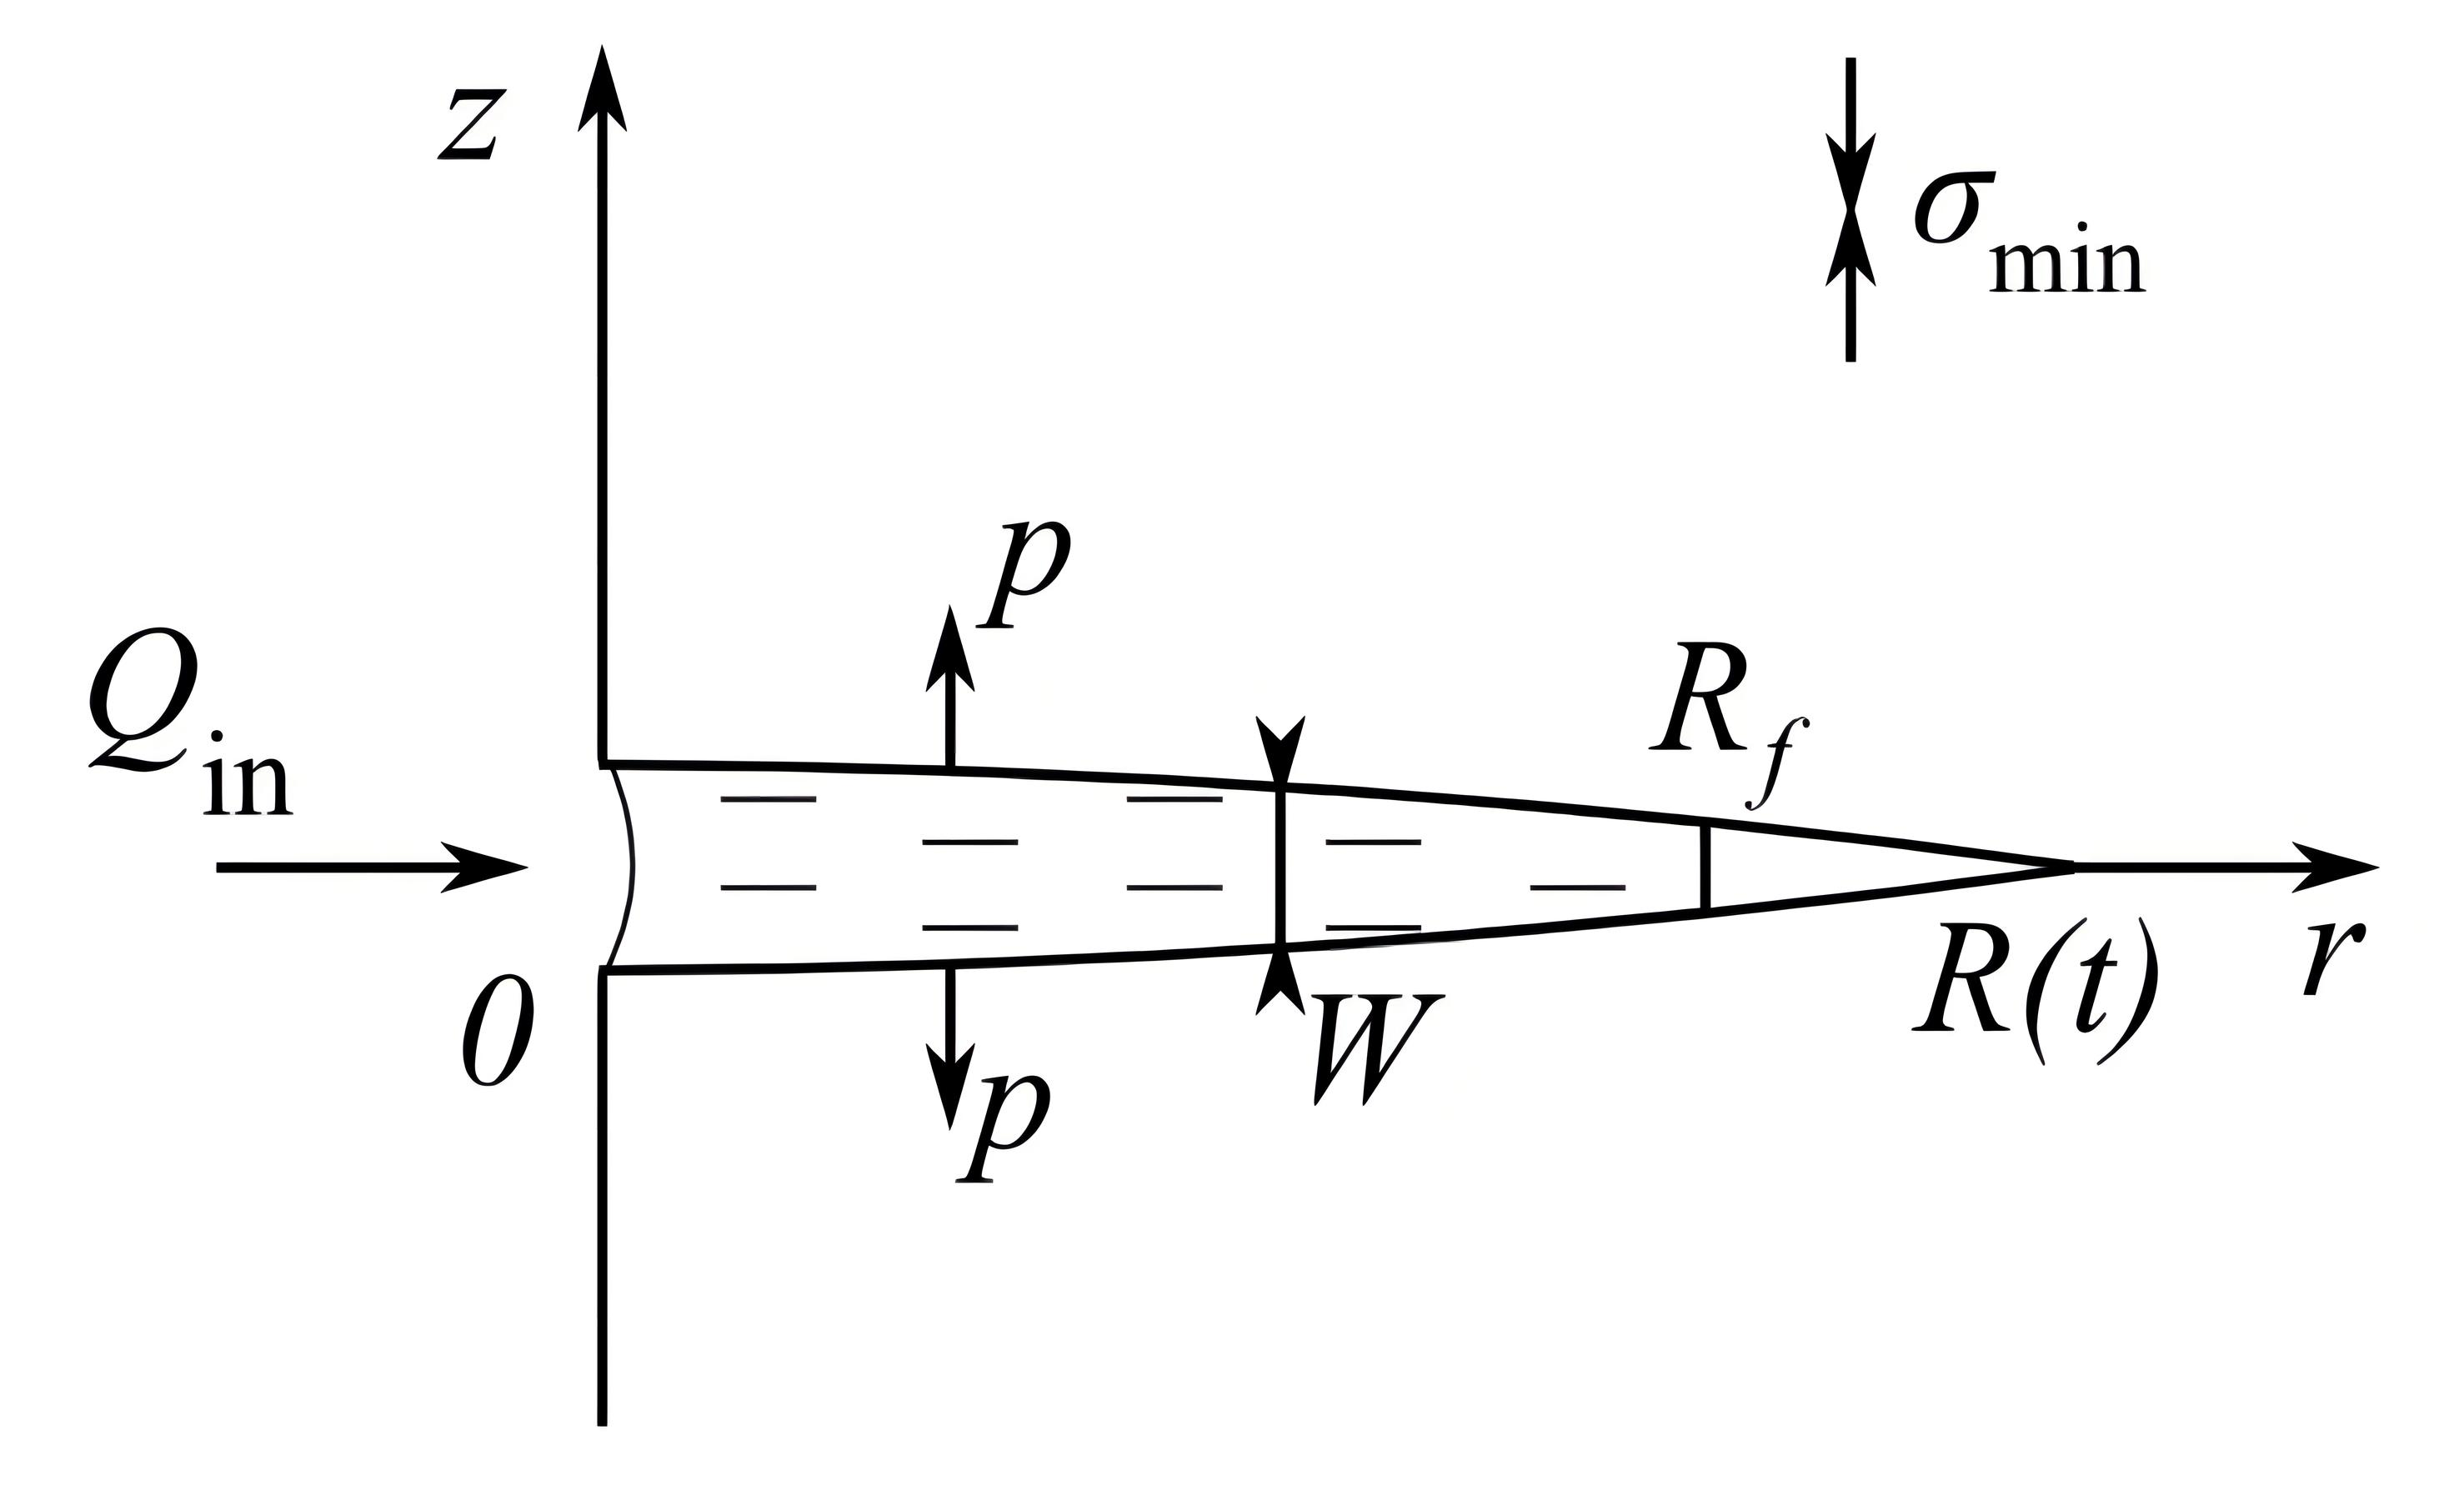
\includegraphics[width=5.2cm]{radial_model_A-A_plane.jpg}
\end{textblock*}

\begin{textblock*}{6cm}(0.5cm,8.7cm)
\tiny
\textcolor{lit_gray}{E.V. Dontsov. An approximate solution for a penny-shaped hydraulic fracture that accounts for fracture toughness, fluid viscosity, and leak-off. \emph{R. Soc. Open Sci.}, 3:160737, 2016}
\end{textblock*}

\normalsize

\end{frame}
\end{comment}


\begin{frame}
\frametitle{Модель Перкинса-Керна-Нордгрена (модель PKN)}

\scriptsize

\begin{textblock*}{7cm}(0.5cm,1cm)
$$
\begin{cases}
\dfrac{\partial\bar{w}}{\partial t}+\dfrac{\partial\bar{q}_x}{\partial x}+\dfrac{C'}{\sqrt{t-t_0(x)}}=\dfrac{Q_0}{H}\delta(x),\\[15pt]
\bar{q}_x=-\dfrac{\bar{w}^3}{\pi^2\mu}\dfrac{\partial p_n}{\partial x},\\[15pt]
p_n(x,t)=\dfrac{2E'}{\pi^2H}\displaystyle\int\limits_{-L(t)}^{L(t)}\bar{w}(x',t)\dfrac{dG(2(x'-x)/H)}{dx'}dx',\\[22pt]
\displaystyle\lim_{x\to L}\dfrac{w}{(L-x)^{1/2}}=\dfrac{K'}{E'},
\end{cases}
$$
где $C'=2C_l$; $\,\,\,\mu'=12\mu$; $\,\,\,E'=\dfrac{E}{1-\nu^2}$; $\,\,\,K'=\dfrac{8K_{Ic}}{\sqrt{2\pi}}$;
\end{textblock*}

\begin{textblock*}{7cm}(0cm,7.2cm)
$$
G(s)=\frac{\sqrt{1+s^2}}{s}\,E\!\left(\frac{1}{1+s^2}\right)
$$
\end{textblock*}

\begin{textblock*}{7cm}(7.4cm,1.5cm)
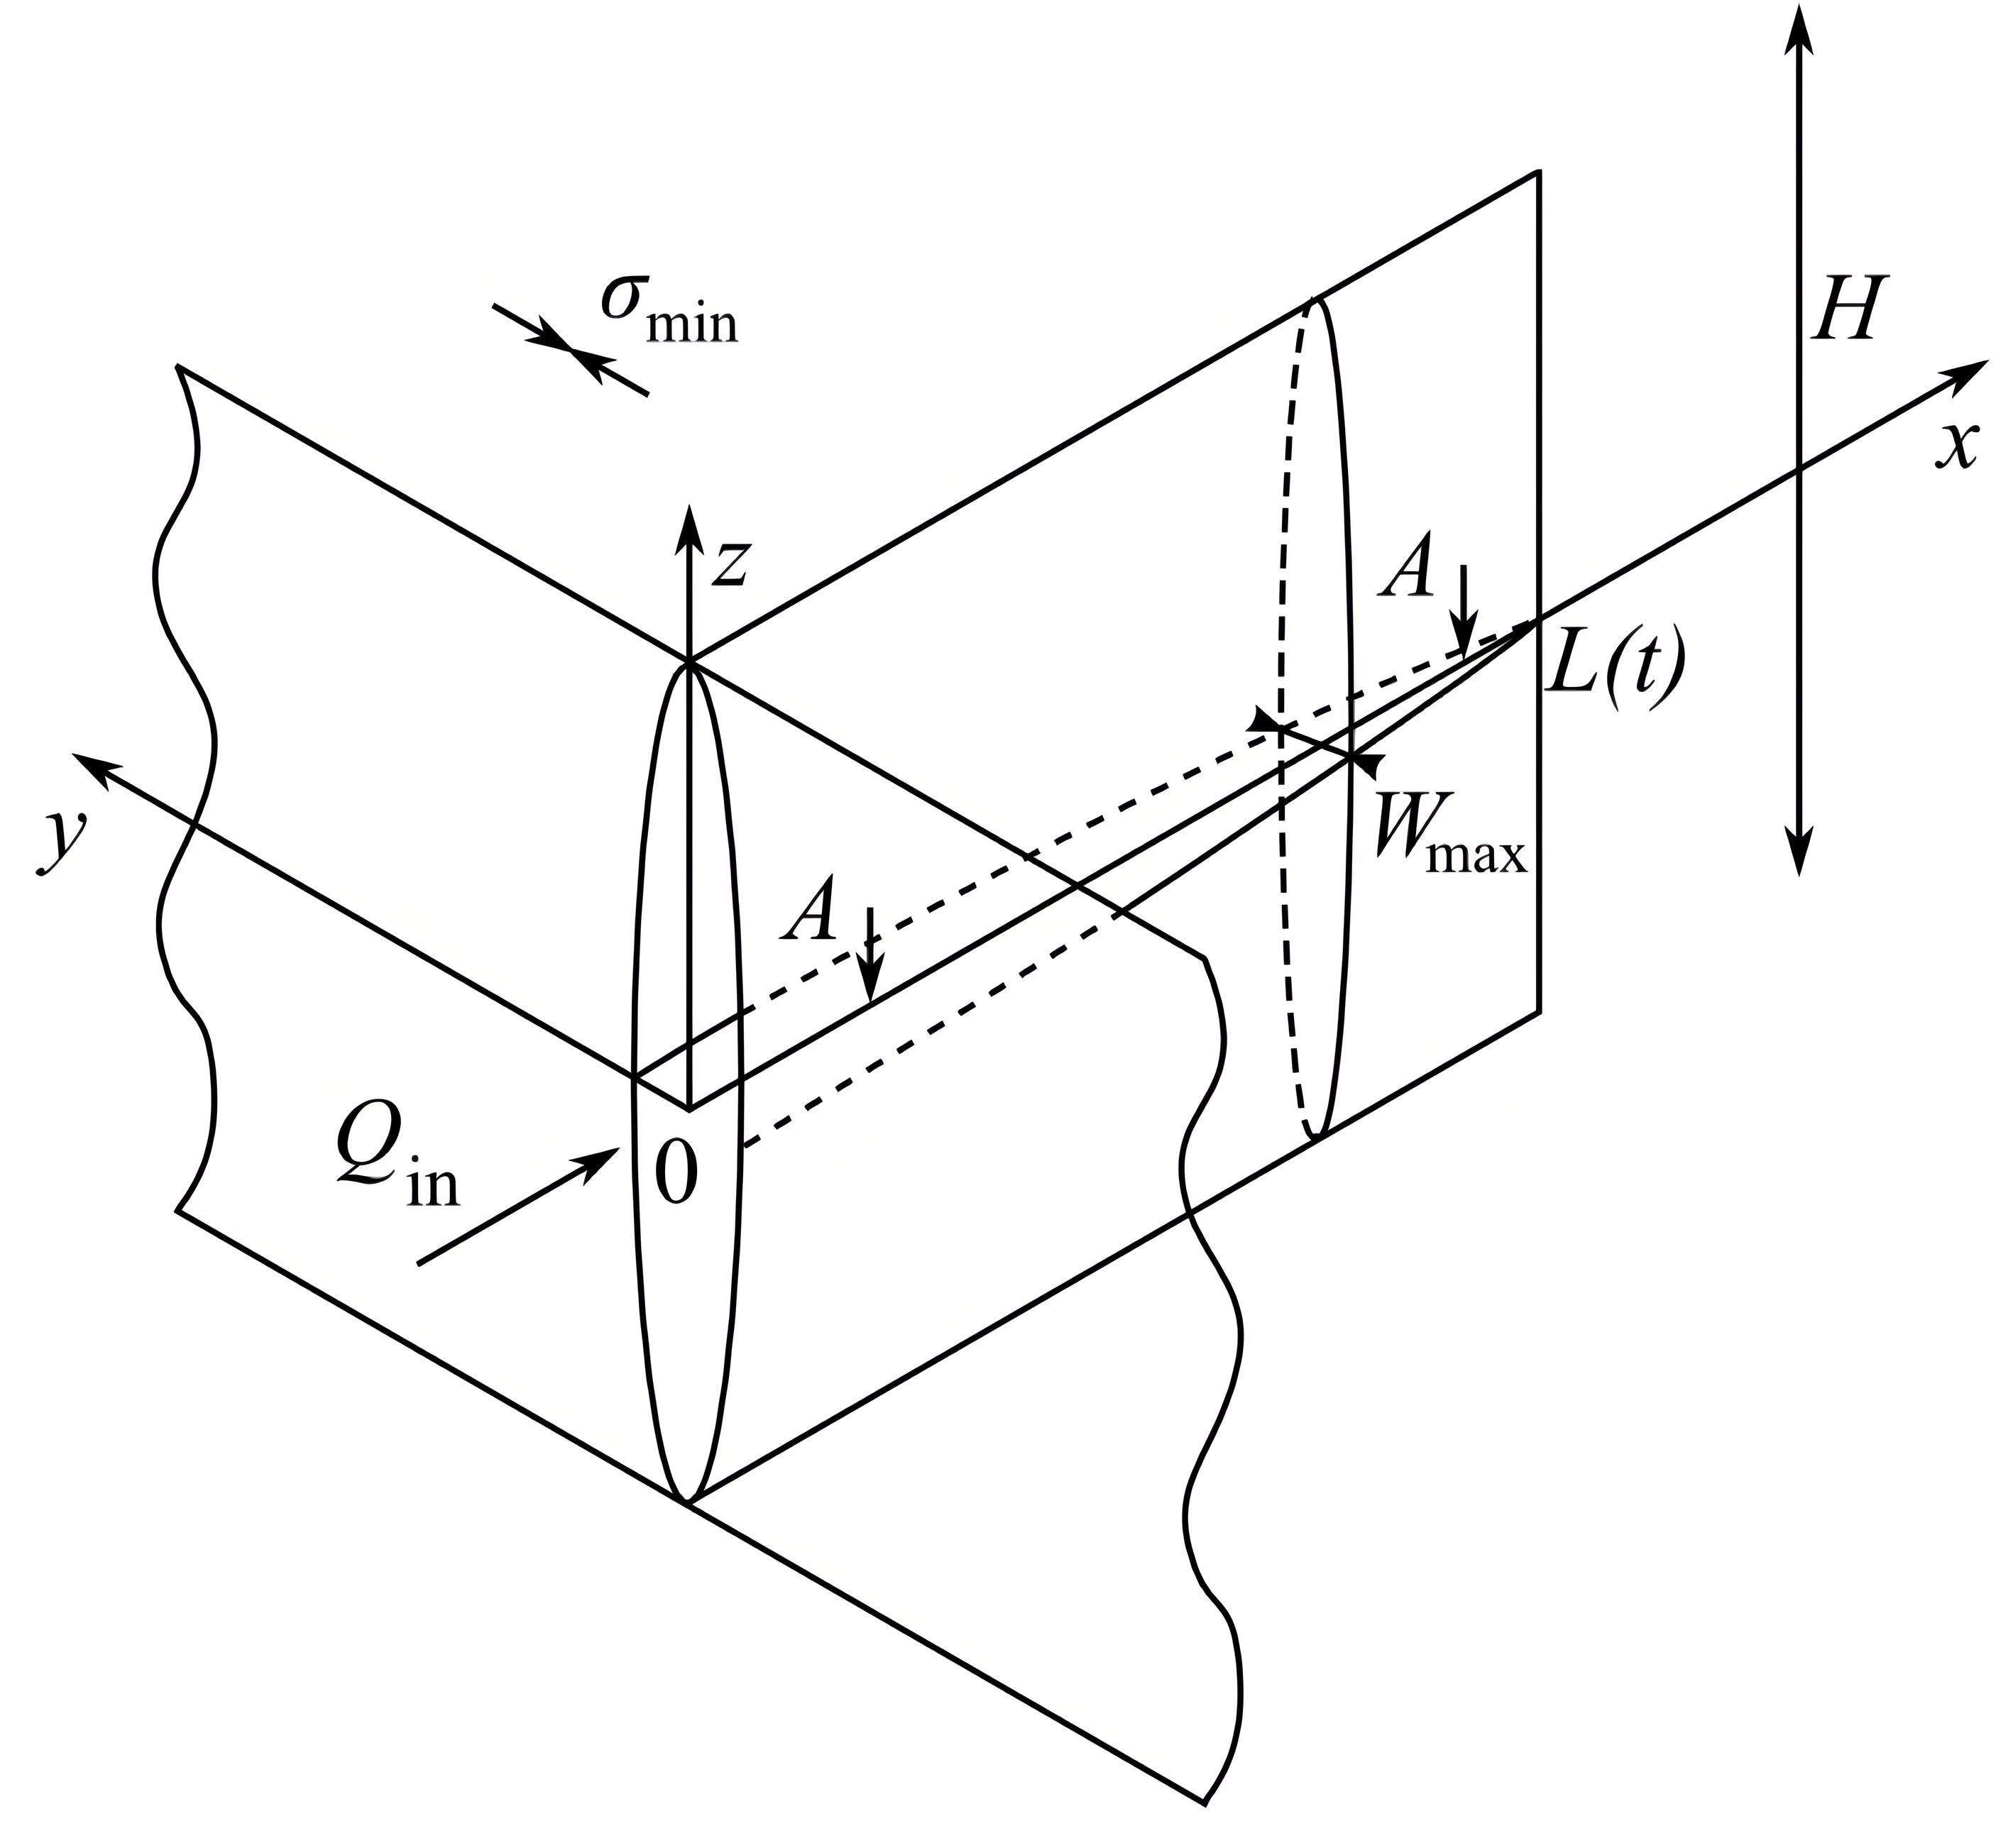
\includegraphics[width=5.2cm]{pkn_model_3D.jpg}
\end{textblock*}

\begin{textblock*}{7cm}(7.5cm,6.3cm)
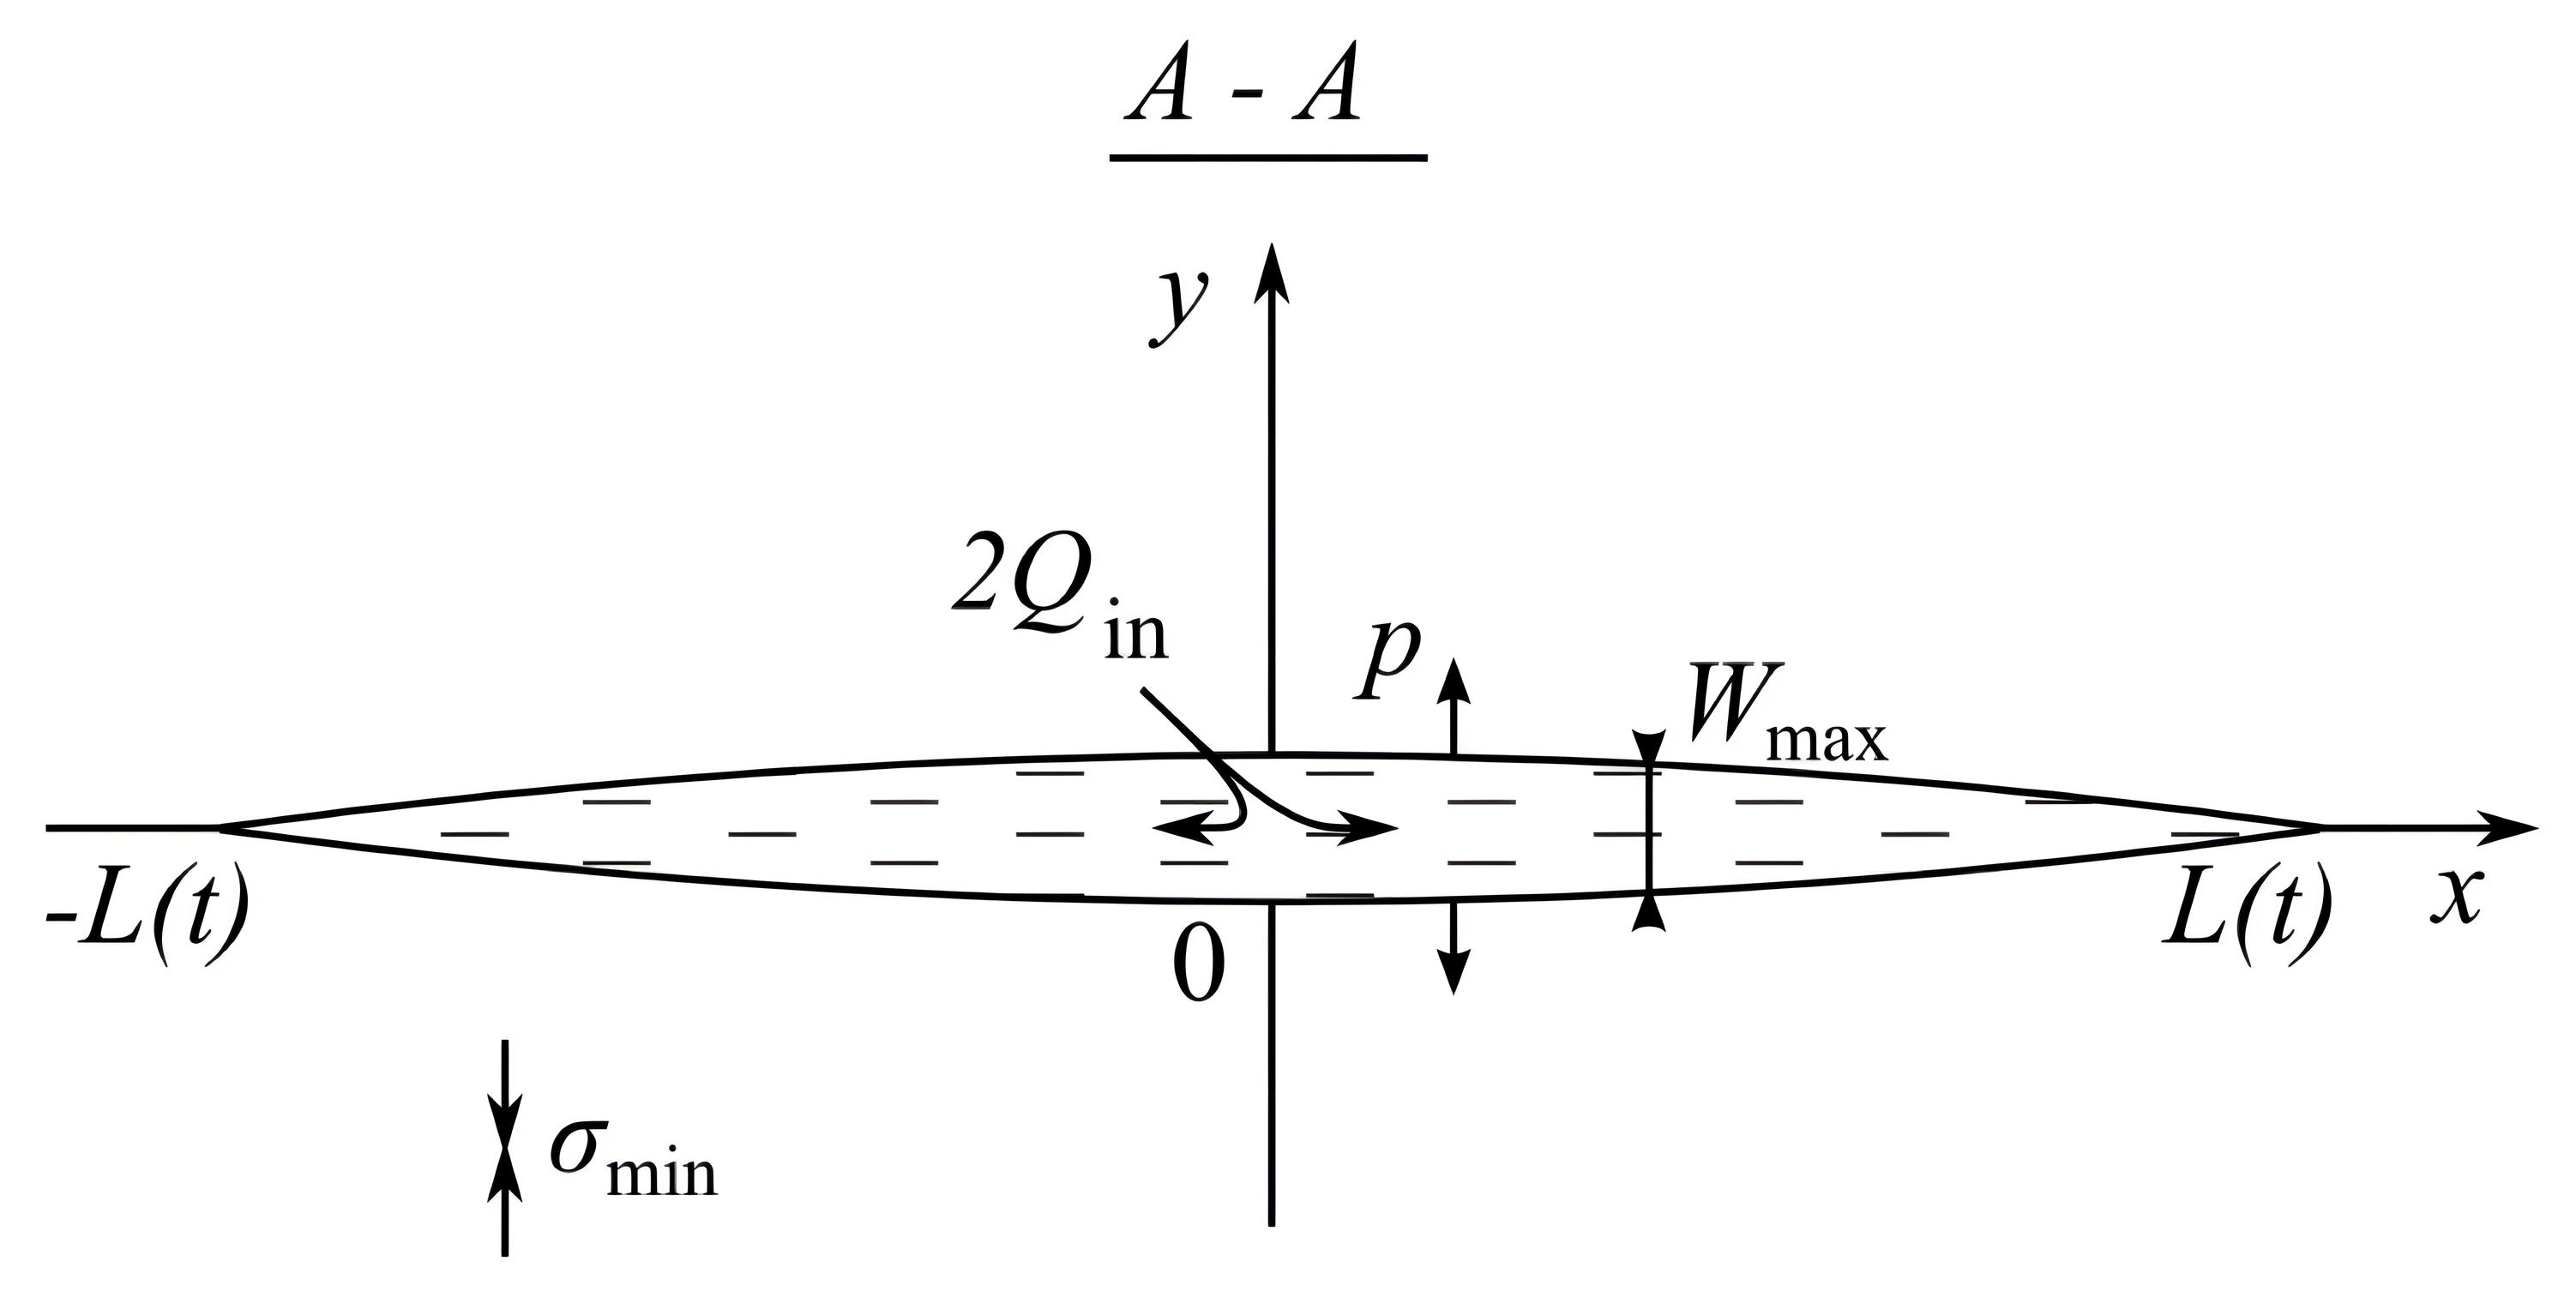
\includegraphics[width=5cm]{pkn_model_A-A_plane.jpg}
\end{textblock*}

\begin{textblock*}{3.7cm}(3.7cm,1.9cm)
\tiny
$$
\boxed{
\bar{w}(x)=\frac{1}{H}\!\int\limits_{-H/2}^{H/2}{w(x,z)dz}
}
$$
\end{textblock*}

\begin{textblock*}{7cm}(5.5cm,1.1cm)
\tiny
$$
\boxed{
w(x,z)=\frac{4}{\pi}\bar{w}(x)\sqrt{1-\left(\frac{2z}{H}\right)^2}
}
$$
\end{textblock*}

\begin{textblock*}{7cm}(0.5cm,8.7cm)
\scriptsize
\textcolor{lit_gray}{E.V. Dontsov. Analysis of a constant height hydraulic fracture, arXiv:2110.13088v1 [physics.geo-ph], 25 Oct 2021}
\end{textblock*}

\normalsize

\end{frame}


\begin{frame}
\frametitle{Формулы Кёнинга}
\small
\begin{textblock*}{11cm}(0.7cm,1.3cm)
\begin{tabular}{|p{4.3cm}|p{5.9cm}|}
\hline
В случае одномерных утечек Картера & В случае двумерных радиальных утечек жидкости из трещины в пласт\\
\hline
$$x_{\!f}=\frac{Q\mu\sqrt{\pi\kappa t}}{2\pi k_eh\left(p_{\!f}-p_e\right)}
\vspace*{-3mm}$$ & $$x_{\!f}=3\exp{\!\left(-\frac{2\pi k_e h\left(p_{\!f}-p_e\right)}{Q\mu}\right)}\sqrt{\kappa t}$$ \\
\hline
\end{tabular}
\end{textblock*}

\begin{textblock*}{11cm}(0.7cm,4.5cm)
где
$\kappa=\dfrac{k_e}{\varphi_e\mu c_t}$ -- пьезопроводность пласта;\newline

$Q$ -- расход нагнетаемой в рассматриваемую трещину жидкости;\newline
$\mu$ -- вязкость жидкости;
$t$ -- время закачки;\newline
$k_e$ и $\varphi_e$ -- проницаемость и пористость пласта соответственно;\newline
$c_t$ -- общая сжимаемость;
$h$ -- эффективная толщина (мощность) пласта;
$\Delta p=p_{\!f}-p_e$ -- разница между средним давлением в трещине и пластовым давлением.
\end{textblock*}
\normalsize

\begin{textblock*}{10cm}(0.7cm,8.7cm)
\scriptsize
\textcolor{lit_gray}{E.J.L. Koning. Fractured water-injection wells. Analytical modelling of fracture propagation. SPE 14684, 1985}
\end{textblock*}

\normalsize

\end{frame}


\begin{comment}
\begin{frame}
\frametitle{Параметрическая карта решения модели PKN}

\begin{textblock*}{7cm}(5.5cm,1.2cm)
\tiny
$$
\Omega=\frac{\bar{w}}{w_{*}}\,\,\,\,\,;\,\,\,\,\,\lambda=\frac{l}{l_{*}}\,\,\,\,\,;\,\,\,\,\,\tau=\frac{t}{t_{*}}\,\,\,\,\,;\,\,\,\,\,\xi=\frac{x}{l(t)}
$$
\normalsize
\end{textblock*}

\begin{textblock*}{7cm}(5.5cm,2.2cm)
\tiny
$$
w_{*}=\frac{\left(\pi H\right)^{1/2}K_{Ic}}{E'}\,\,\,\,\,;\,\,\,\,\,l_{*}=\frac{H^2K_{Ic}^4}{2\pi E'^3\mu Q_0}
$$
\normalsize
\end{textblock*}

\begin{textblock*}{7cm}(5.5cm,3.2cm)
\tiny
$$
t_{*}=\frac{H^{7/2}K_{Ic}^5}{2\pi^{1/2}E'^4\mu Q_0^2}\,\,\,\,\,;\,\,\,\,\,\phi=\left(\frac{H^5K_{Ic}^6C'^4}{4\pi^3E'^4\mu^2Q_0^4}\right)^{1/4}
$$
\normalsize
\end{textblock*}

\begin{textblock*}{6cm}(6cm,4.5cm)
\scriptsize
\textcolor{red}{
$K$-режим = доминирование трещиностойкости и отсутствие утечек (пренебрегаем вязкостью)
}
\normalsize
\end{textblock*}

\begin{textblock*}{6cm}(6cm,5.6cm)
\scriptsize
\textcolor{magenta}{
$\tilde{K}$-режим = доминирование трещиностойкости и большие утечки (пренебрегаем вязкостью)
}
\normalsize
\end{textblock*}

\begin{textblock*}{6.5cm}(6cm,6.8cm)
\scriptsize
\textcolor{blue}{
$M$-режим = доминирование вязкости и отсутствие утечек (пренебрегаем трещиностойкостью)
}
\normalsize
\end{textblock*}

\begin{textblock*}{6cm}(6cm,7.8cm)
\scriptsize
\textcolor{new_green}{
$\tilde{M}$-режим = доминирование вязкости и большие утечки (пренебрегаем трещиностойкостью)
}
\normalsize
\end{textblock*}

\begin{textblock*}{4.5cm}(0.5cm,5.2cm)
\scriptsize
\renewcommand{\baselinestretch}{0.7}
В данной работе предполагается, что трещины автоГРП распространяются в режиме больших утечек и доминирования трещиностойкости (пренебрегаем вязкостью).
В этом режиме решение для среднего раскрытия:
\vspace*{-3mm}
$$
\bar{w}_{\tilde{K}}=\frac{K_{Ic}\sqrt{\pi H}}{E'}
$$
\normalsize
\end{textblock*}



\begin{textblock*}{5cm}(0.5cm,1.1cm)
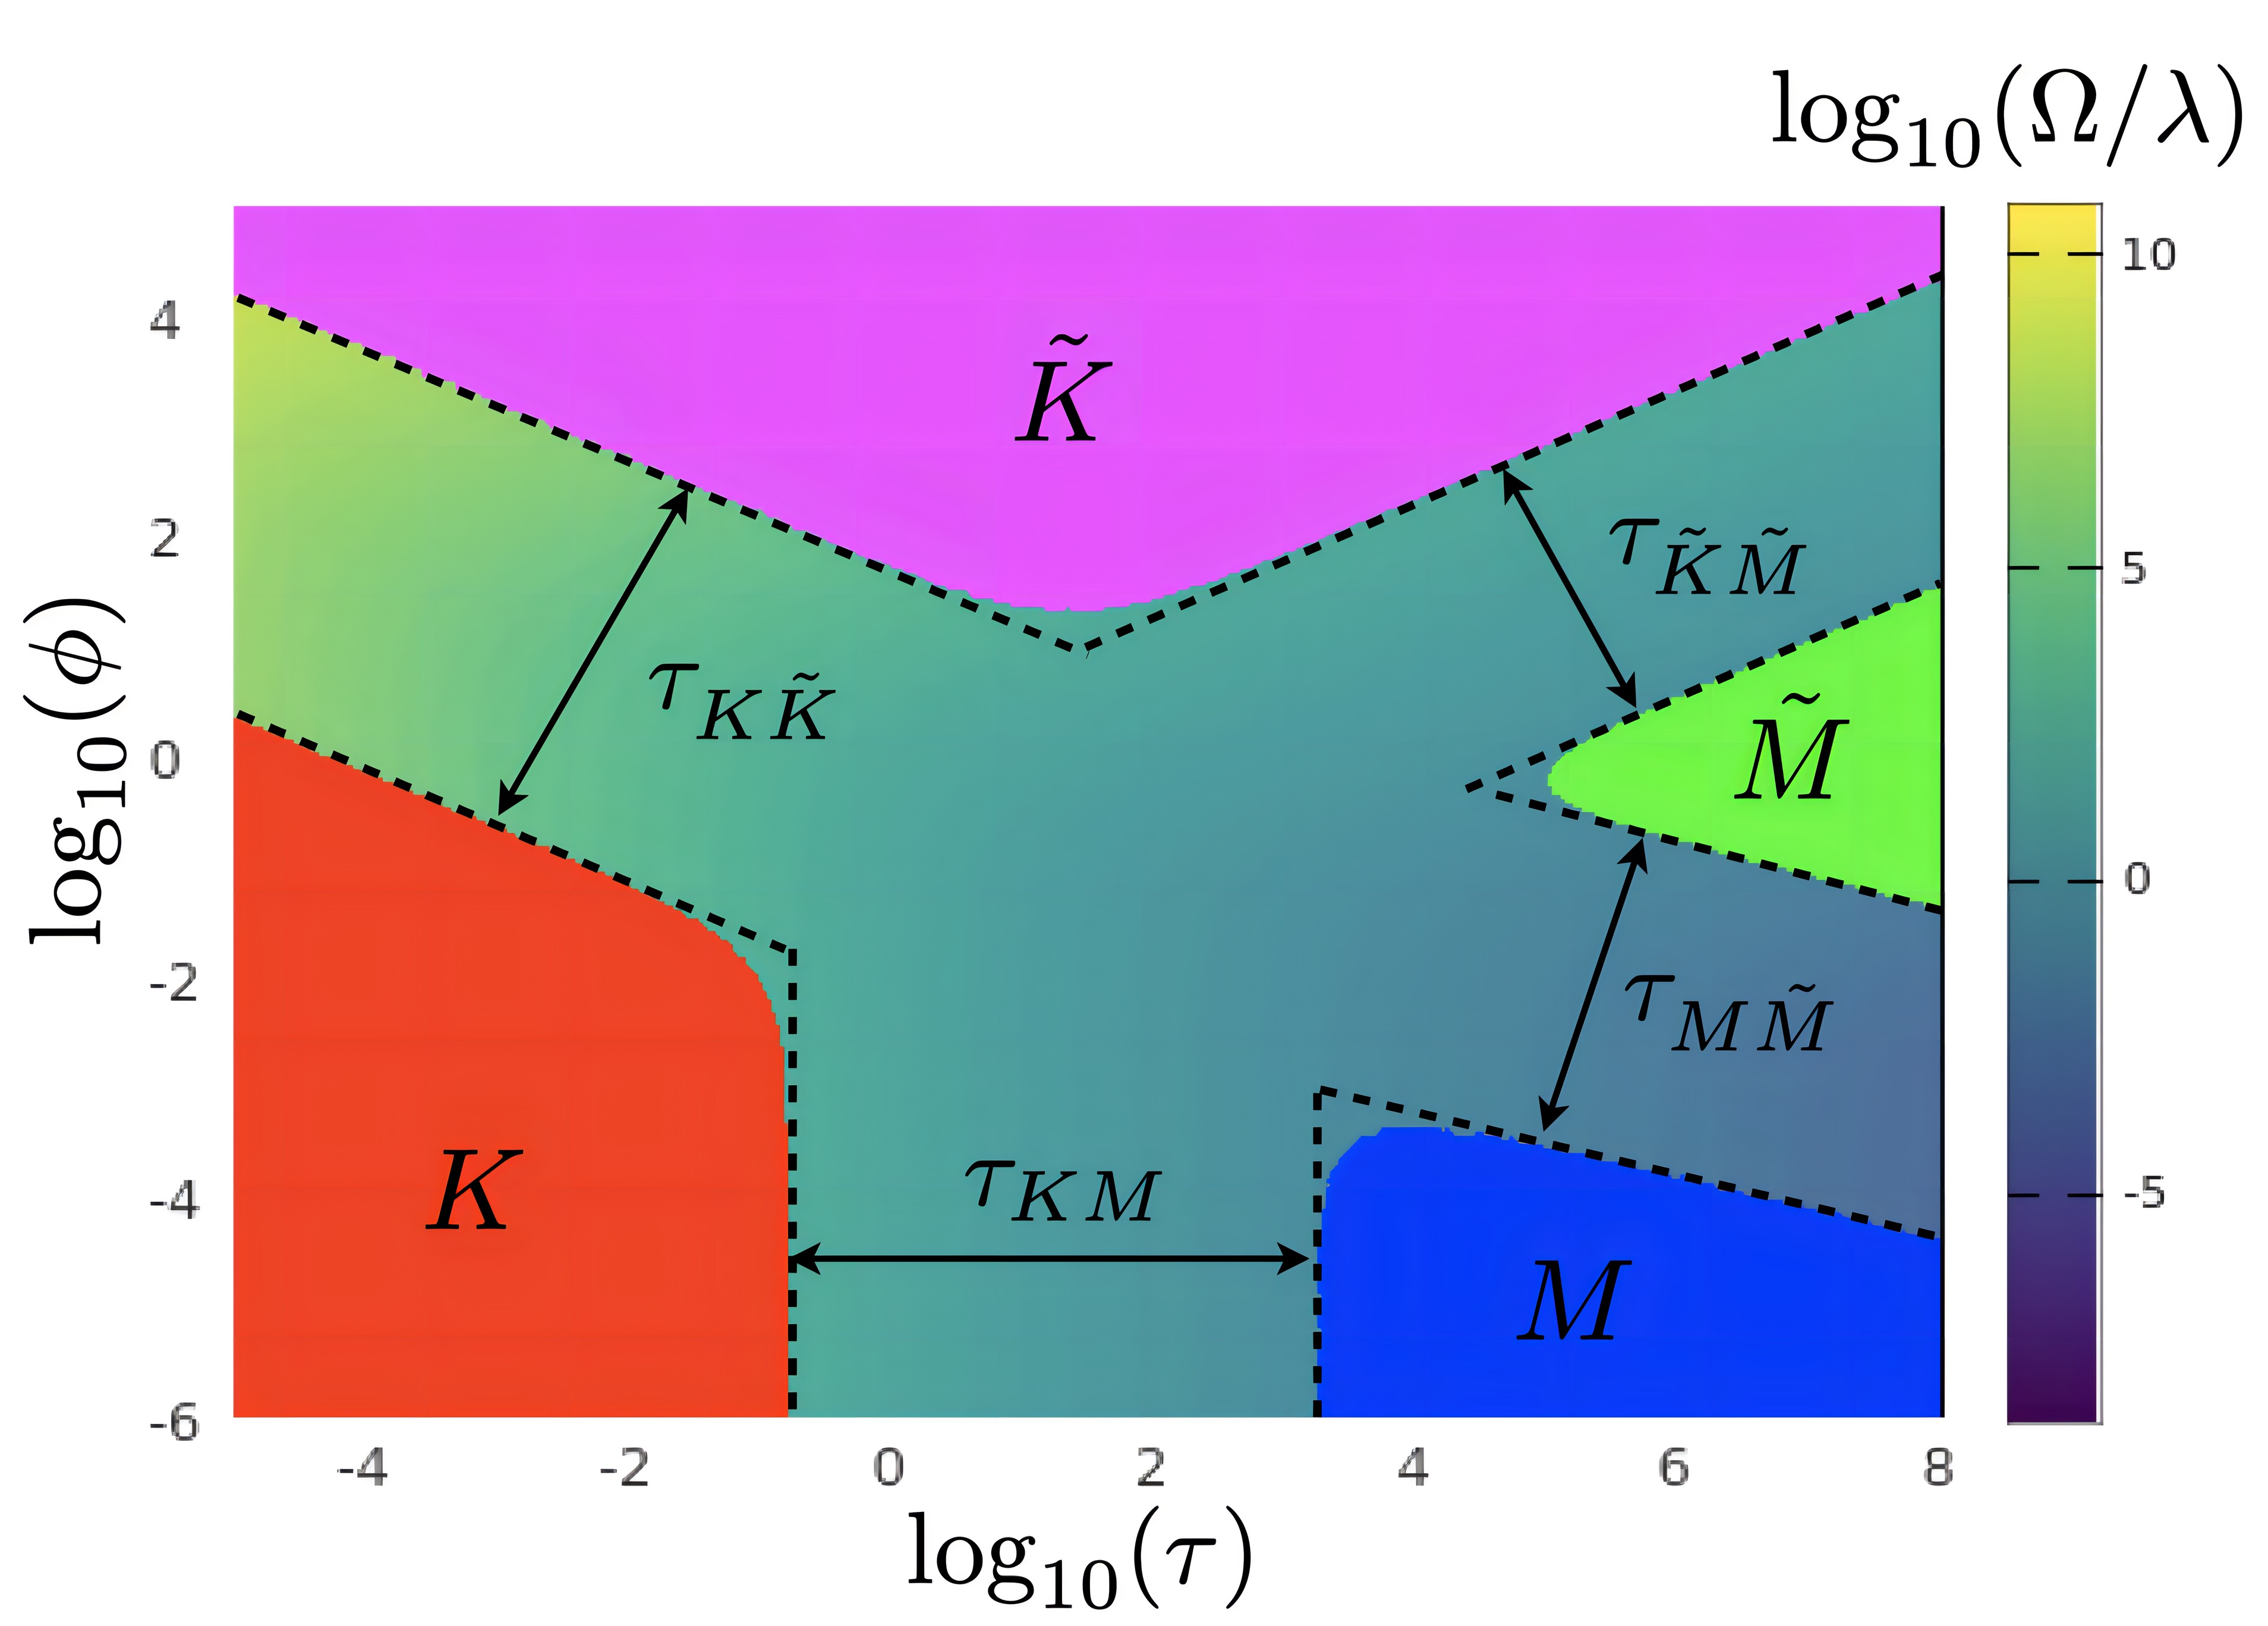
\includegraphics[width=5cm]{pkn_parametric_space.jpg}
\end{textblock*}

\begin{textblock*}{6cm}(0.5cm,8.9cm)
\tiny
\textcolor{lit_gray}{E.V. Dontsov. Analysis of a constant height hydraulic fracture, arXiv:2110.13088v1 [physics.geo-ph], 25 Oct 2021}
\end{textblock*}

\end{frame}
\end{comment}


\begin{frame}
\frametitle{Схема перераспределения потоков между трещинами гидроразрыва и правила Кирхгофа}

\begin{textblock*}{11cm}(1cm,1.5cm)
%\tiny Подпись к рисунку
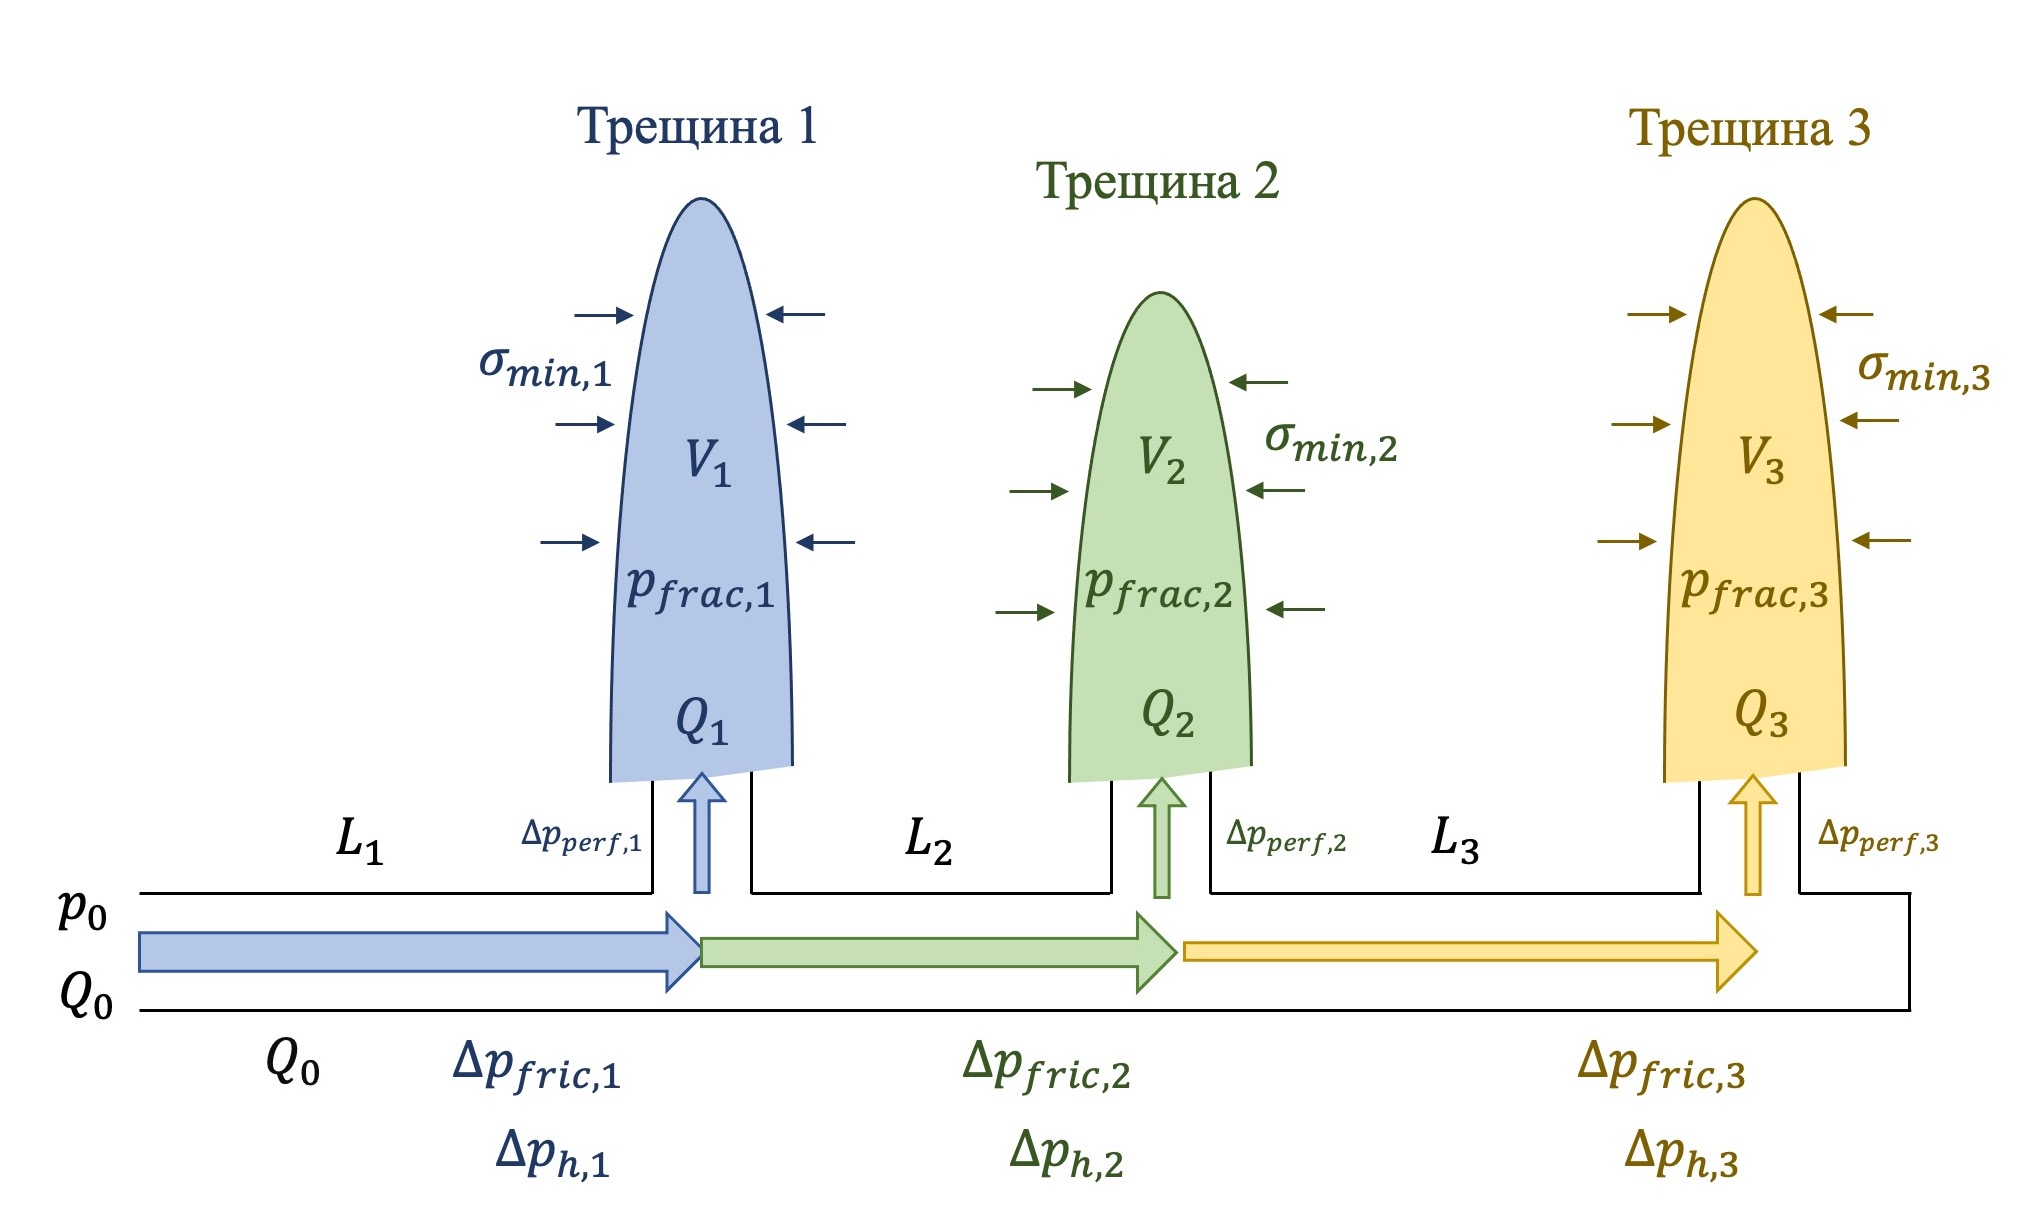
\includegraphics[width=10cm]{flow_distribution_scheme.jpg}
\end{textblock*}

\begin{textblock*}{4cm}(-0.2cm,7.5cm)
$$\boxed{Q_0=\sum\limits_{i=1}^{N}Q_i}$$
\end{textblock*}

\begin{textblock*}{11cm}(2.2cm,7.5cm)
$$\boxed{p_0=\underbrace{\sigma_{\text{min},i}+p_{\text{net},i}}_{p_{\text{frac},i}}+\Delta p_{\text{perf},i}-\sum_{j=1}^{i}{\Delta p_{h,\,j}}+\sum_{j=1}^{i}\Delta p_{\text{fric},\,j}}$$
\end{textblock*}

\end{frame}


\begin{frame}
\frametitle{Замыкающие соотношения}
\footnotesize

\begin{textblock*}{11cm}(0.7cm,1cm)
\begin{tabular}{|C{5.5cm}|C{4.9cm}|}
\hline
Чистое давление в распространяющихся трещинах PKN (условие роста трещин)& \vspace*{-4.5mm}$$p_{\text{net},i}=\sqrt{\frac{8K_{Ic,i}^2}{\pi h_{f,i}}}$$\vspace*{-3mm}\\
\hline
Падение давления на перфорациях & \vspace*{-4mm}$$\Delta p_{\text{perf},i}=\frac{8\rho_s}{\pi^2\,C_{d,i}^2\,n_{p,i}^2 \,d_{p,i}^4}Q_i\left|Q_i\right|$$ \vspace*{-3mm}\\
\hline
Падение давления на трение при ламинарном режиме течения & \vspace*{-4mm}$$\Delta p_{\text{fric}, i}=\int\limits_{x_{i-1}}^{x_i}{\frac{8\mu\left(Q_0-\sum\limits_{j=1}^{i-1}{Q_j}\right)}{R_i^2(s)S_i(s)}}ds$$ \vspace*{-4mm}\\
\hline
\end{tabular}
\end{textblock*}


\begin{textblock*}{11.2cm}(0.7cm,5.55cm)
\scriptsize
$K_{Ic,i}$ -- трещиностойкость породы вблизи кончика $i$-ой трещины;
$h_{f,i}=H$ -- высота трещин (для PKN модели равна мощности пласта);\\
$\rho_s$ и $\mu$ -- плотность и вязкость закачиваемой жидкости соответственно;\\
$n_{p,i}$ и $d_{p,i}$ -- количество и диаметр перфораций соответственно;
$C_{d,i}$ -- безразмерный коэффициент эрозии перфораций (при закачке воды равен 0.5);\\
$Q_0$ -- расход закачиваемой жидкости на забое;
$Q_j$ -- расход жидкости на $j$-ой трещине;\\
$R_i$ -- радиус участка трубы к $i$-ой трещине;\\
$S_i=\pi R_i^2$ -- площадь сечения участка трубы к $i$-ой трещине.
\end{textblock*}

\begin{textblock*}{11.2cm}(0.7cm,8.4cm)
\tiny
\textcolor{lit_gray}{P.A. Kabanova, E.V. Shel. Modeling of Water-Induced Fracture Growth Pressure Using Poroelastic Approach. — ECMOR XVII – 17th European Conference on the Mathematics of Oil Recovery, 2020}
\end{textblock*}

\begin{textblock*}{11.2cm}(0.7cm,9.0cm)
\tiny
\textcolor{lit_gray}{J.B. Crump, M.W. Conway. Effects of Perforation-Entry Friction on Bottomhole Treating Analysis. — Journal of Petroleum Technology, August 1988}
\end{textblock*}

\normalsize

\end{frame}

\begin{comment}
\begin{frame}
\frametitle{Падение давления на перфорациях}
\begin{textblock*}{11cm}(1cm,2cm)
$$
\Delta p_{\text{perf},i}=\frac{8\rho_s}{\pi^2\,C_{d,i}^2\,n_{p,i}^2 \,d_{p,i}^4}Q_i\left|Q_i\right|
$$\\
где $\rho_s$ -- плотность жидкости;\newline
$n_{p,i}, d_{p,i}$ -- количество и диаметр перфораций;\newline\\
$C_{d,i}$ -- безразмерный коэффициент эрозии (в случае отсутствия твёрдых частичек в потоке $C_{d,i}\in\left[0.5,0.6\right]$, а с твёрдыми частичками в потоке $C_{d,j}\in\left[0.6,0.95\right]$  из-за эрозии перфорации).
\end{textblock*}

\begin{textblock*}{11cm}(1cm,7.5cm)
\scriptsize
\textcolor{lit_gray}{J.B. Crump, M.W. Conway. Effects of Perforation-Entry Friction on Bottomhole Treating Analysis. — Journal of Petroleum Technology, August 1988}
\end{textblock*}

\begin{textblock*}{11cm}(1cm,8.5cm)
\scriptsize
\textcolor{lit_gray}{G. Long, S. Liu, G. Xu, S.-W. Wong. Modeling of Perforation Erosion for Hydraulic Fracturing Applications. — SPE-174959-MS, 2015.}
\end{textblock*}

\normalsize

\end{frame}


\begin{frame}
\frametitle{Падение давления на трение при ламинарном режиме течения}
\begin{textblock*}{11cm}(1cm,2cm)
$$
\Delta p_{\text{fric}, i}=\int\limits_{x_{i-1}}^{x_i}{\frac{8\mu\left(Q_0-\sum\limits_{j=1}^{i-1}{Q_j}\right)}{R_i^2(s)S_i(s)}}ds,
$$\\
где $\mu$ -- вязкость жидкости;\newline
$Q_0$ -- расход закачиваемой жидкости на забое;\newline
$Q_j$ -- расход жидкости на $j$-ой трещине;\newline
$R_i$ -- радиус участка трубы к $i$-ой трещине;\newline
$S_i=\pi R_i^2$ -- площадь сечения участка трубы к $i$-ой трещине.
\end{textblock*}
\normalsize
\end{frame}
\end{comment}


\begin{frame}
\frametitle{Замкнутая постановка задачи}
\small
\begin{textblock*}{11cm}(0.3cm,1.5cm)
$$
\begin{cases}
	\displaystyle Q_0=\sum\limits_{i=1}^{N}Q_i,\\
	\displaystyle p_0=\sigma_{\text{min},i}+p_{\text{net},i}+\Delta p_{\text{perf},i}-\sum_{j=1}^{i}{\Delta p_{h,j}}+\sum_{j=1}^{i}\Delta p_{\text{fric},j},\\[10pt]
	\displaystyle p_{\text{net},i}=\sqrt{\dfrac{8K_{Ic,i}^2}{\pi h_{f,i}}},\\[15pt]
	\displaystyle \Delta p_{\text{perf},i}=\dfrac{8\rho_s}{\pi^2 C_{d,i}^2 n_{p,i}^2 d_{p,i}^4}Q_i\left|Q_i\right|,\\[15pt]
	\displaystyle \Delta p_{\text{fric}, j}=\int\limits_{x_{j-1}}^{x_j}{\dfrac{8\mu\left(Q_0-\sum\limits_{k=1}^{j-1}{Q_k}\right)}{R_j^2(s)S_j(s)}}ds,\\[20pt]
	\displaystyle \Delta p_{h,j}=0.
\end{cases}
$$
\end{textblock*}

\begin{textblock*}{11cm}(8cm,5cm)
	\fbox{\begin{minipage}{9em}
		Неизвестные:\\$Q_1$, $Q_2$, ..., $Q_N$, $p_0$.
	\end{minipage}}
\end{textblock*}

\normalsize
\end{frame}


\begin{frame}
\frametitle{Вектор невязок}

Вектор неизвестных:
$$Q^T=\left[Q_1,Q_2,...,Q_N,p_0\right]$$

Вектор невязок:
$$\left[F_1,F_2,...,F_N,F_{N+1}\right],$$
где
$$
F_i=
\begin{cases}
\sigma_{\text{min},i}+p_{\text{net},i}+\Delta p_{\text{perf},i}-\sum\limits_{j=1}^{i}{\Delta p_{h,j}}+\sum\limits_{j=1}^{i}{\Delta p_{\text{fric},j}}-p_0\\\,\,\,\,\,\,\,\,\,\,\,\,\,\,\,\,\,\,\,\,\,\,\,\,\,\,\,\,\,\,\,\,\left(\text{при }i\leqslant N\right)\\\ \\
Q_0-\sum\limits_{j=1}^{N}{Q_j}\left(\text{при }i=N+1\right)
\end{cases}
$$

\end{frame}


\begin{frame}
\frametitle{Итеративная процедура решения}
Матрица Якоби:
$$J = \begin{bmatrix}
	\dfrac{\partial F_1}{\partial Q_1} & \dots & \dfrac{\partial F_1}{\partial Q_N} & \dfrac{\partial F_1}{\partial p_0} \\
	\vdots & \ddots & \vdots & \vdots \\
	\dfrac{\partial F_{N+1}}{\partial Q_1} & \dots & \dfrac{\partial F_{N+1}}{\partial Q_N} & \dfrac{\partial F_{N+1}}{\partial p_0} \\
	\end{bmatrix}
$$

Выражение:
$$\overline{Q}^{k+1}=\overline{Q}^k-J^{-1}\overline{F}^k$$
\ \\

Начальное приближение:
$Q_i=Q_0/N\text{ и }p_0=\sigma_i\text{ при } i\in\left[1,N\right]$
\ \\

Условие остановки:
$\left|\overline{Q}^{k+1}-\overline{Q}^k\right|^2\leqslant10^{-4}$

\end{frame}


\begin{frame}
\frametitle{Итеративный процесс поиска расходов на трещинах и забойного давления}

\begin{textblock*}{11.6cm}(0.7cm,2.3cm)
%\tiny Подпись к рисунку
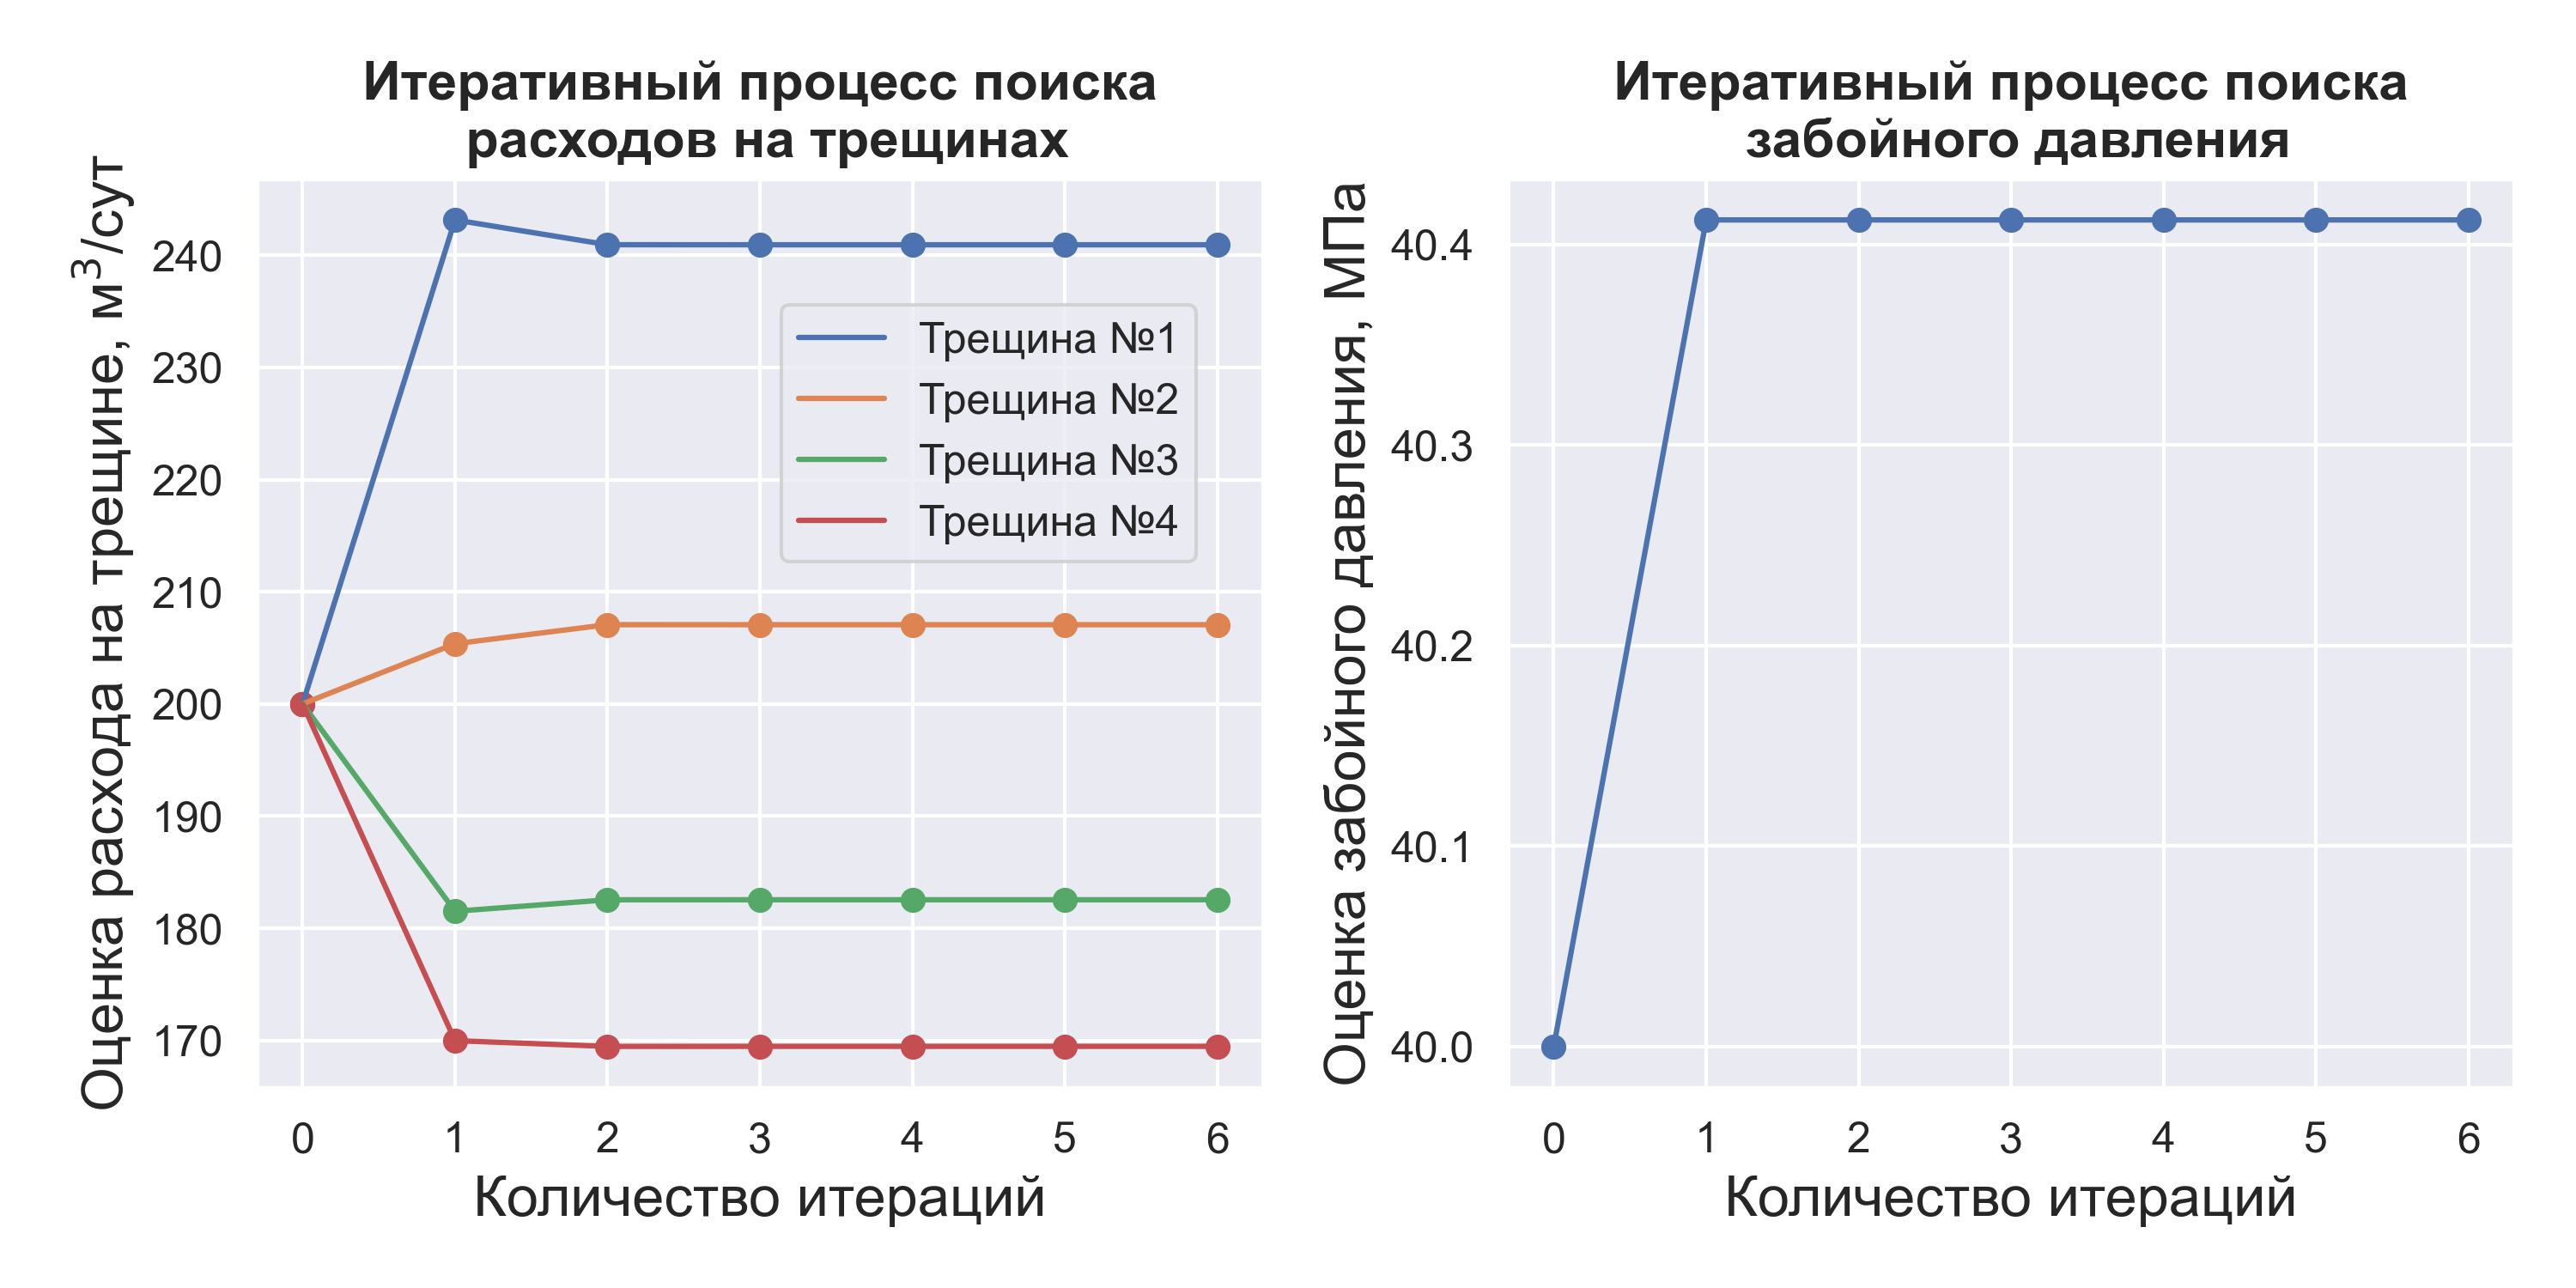
\includegraphics[width=11.6cm]{flows_distribution_between_fractures_1.jpg}
\end{textblock*}

\end{frame}


\begin{frame}
\frametitle{Распределение давления вдоль горизонтального участка скважины}

\begin{textblock*}{11cm}(1cm,1.7cm)
%\tiny Подпись к рисунку
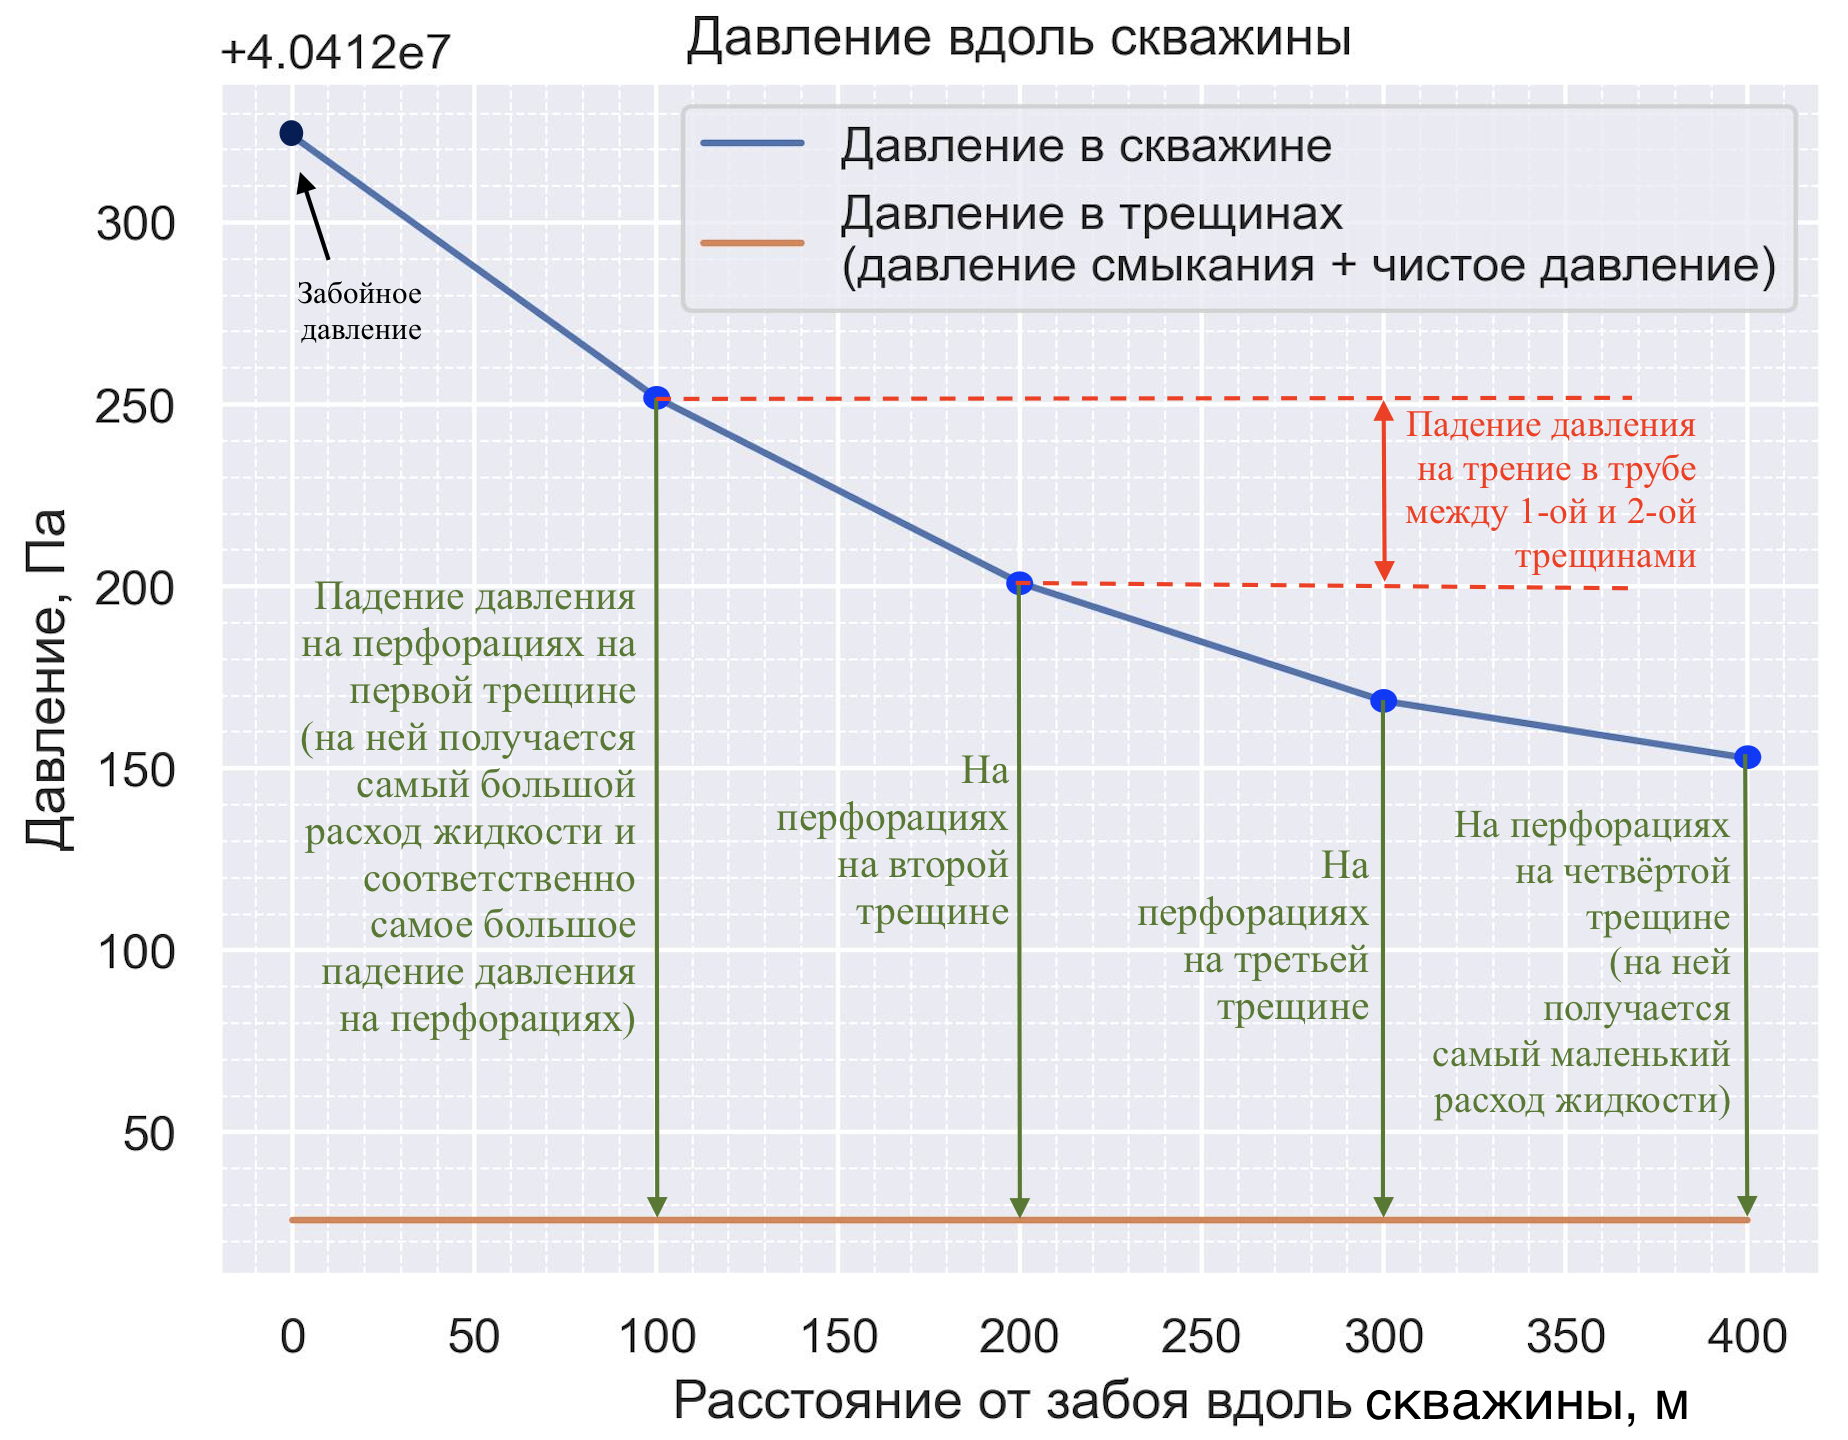
\includegraphics[width=9.5cm]{pressure_distribution.jpg}
\end{textblock*}

\end{frame}

%\begin{frame}
%\frametitle{Пример результатов решателя уравнений Кирхгофа}

%\end{frame}

\begin{comment}
\begin{frame}
\frametitle{Формулы Кёнинга}
\small
\begin{textblock*}{11cm}(0.7cm,1.3cm)
\begin{tabular}{|p{4.3cm}|p{5.9cm}|}
\hline
В случае одномерных утечек Картера & В случае двумерных радиальных утечек жидкости из трещины в пласт\\
\hline
$$x_{\!f}=\frac{Q\mu\sqrt{\pi\kappa t}}{2\pi k_eh\left(p_{\!f}-p_e\right)}
\vspace*{-3mm}$$ & $$x_{\!f}=3\exp{\!\left(-\frac{2\pi k_e h\left(p_{\!f}-p_e\right)}{Q\mu}\right)}\sqrt{\kappa t}$$ \\
\hline
\end{tabular}
\end{textblock*}

\begin{textblock*}{11cm}(0.7cm,4.5cm)
где
$\kappa=\dfrac{k_e}{\varphi_e\mu c_t}$ -- пьезопроводность пласта;\newline

$Q$ -- расход нагнетаемой в рассматриваемую трещину жидкости;\newline
$\mu$ -- вязкость жидкости;
$t$ -- время закачки;\newline
$k_e$ и $\varphi_e$ -- проницаемость и пористость пласта соответственно;\newline
$c_t$ -- общая сжимаемость;
$h$ -- эффективная толщина (мощность) пласта;
$\Delta p=p_{\!f}-p_e$ -- разница между средним давлением в трещине и пластовым давлением.
\end{textblock*}
\normalsize

\begin{textblock*}{10cm}(0.7cm,8.7cm)
\scriptsize
\textcolor{lit_gray}{E.J.L. Koning. Fractured water-injection wells. Analytical modelling of fracture propagation. SPE 14684, 1985}
\end{textblock*}

\normalsize


\end{frame}
\end{comment}


\begin{frame}
\frametitle{Полная производная полудлины трещин по времени}
\small
\begin{textblock*}{11cm}(0.7cm,1.3cm)
Общий вид полной производной полудлины трещины $x_{\!f}$ по времени $t$:
$$
\frac{dx_{\!f}}{dt}=\frac{\partial x_{\!f}}{\partial t}+\frac{\partial x_{\!f}}{\partial Q}\frac{dQ}{dt}+\frac{\partial x_{\!f}}{\partial (p_{\!f}-p_e)}\frac{d(p_{\!f}-p_e)}{dt}
$$

Полная производная полудлины трещины $x_{\!f}$ по времени $t$ в случае одномерных утечек Картера:
$$
\frac{dx_{\!f}}{dt}=\frac{\mu}{2\pi k_e h(p_{\!f}-p_e)}\left(\frac{Q}{2}\sqrt{\frac{\pi\kappa}{t}}+\sqrt{\pi\kappa t}\,\frac{dQ}{dt}-\frac{Q\sqrt{\pi\kappa t}}{\left(p_{\!f}-p_e\right)}\frac{d(p_{\!f}-p_e)}{dt}\right)
$$

Полная производная полудлины трещины $x_{\!f}$ по времени $t$ в случае двумерных радиальных утечек жидкости из трещины в пласт:
$$
\begin{gathered}
\frac{dx_{\!f}}{dt}=\exp{\!\left(-\frac{2\pi k_e h\left(p_{\!f}-p_e\right)}{Q\mu}\right)}\left(\frac{3}{2}\sqrt{\frac{\kappa}{t}}\,+\right.\\[10pt]
+\left.\frac{6\pi k_e h\left(p_{\!f}-p_e\right)}{Q^2\mu}\sqrt{\kappa t}\,\frac{dQ}{dt}-\frac{6\pi k_e h}{Q\mu}\sqrt{\kappa t}\,\frac{d(p_{\!f}-p_e)}{dt}\right)
\end{gathered}
$$
\end{textblock*}
\end{frame}


\begin{frame}
\frametitle{Приращение полудлины трещин}
\small
\begin{textblock*}{11cm}(0.7cm,1.3cm)
Приращение полудлины трещины на каждом шаге по времени в общем виде:
$$
dx_{\!f}=\frac{dx_{\!f}}{dt}dt
$$
Приращение полудлины трещины на каждом шаге по времени в случае одномерных утечек Картера:
$$
dx_{\!f}=\frac{\mu}{2\pi k_e h(p_{\!f}-p_e)}\left(\frac{Q}{2}\sqrt{\frac{\pi\kappa}{t}}dt+\sqrt{\pi\kappa t}\,dQ-\frac{Q\sqrt{\pi\kappa t}}{\left(p_{\!f}-p_e\right)}d(p_{\!f}-p_e)\right)
$$
Приращение полудлины трещины на каждом шаге по времени в случае двумерных радиальных утечек жидкости из трещины в пласт:
$$
\begin{gathered}
dx_{\!f}=\exp{\!\left(-\frac{2\pi k_e h\left(p_{\!f}-p_e\right)}{Q\mu}\right)}\left(\frac{3}{2}\sqrt{\frac{\kappa}{t}}dt\,+\right.\\[10pt]
+\left.\frac{6\pi k_e h\left(p_{\!f}-p_e\right)}{Q^2\mu}\sqrt{\kappa t}\,dQ-\frac{6\pi k_e h}{Q\mu}\sqrt{\kappa t}\,d(p_{\!f}-p_e)\right)
\end{gathered}
$$
\end{textblock*}
\normalsize

\end{frame}


\begin{frame}
\frametitle{Алгоритм расчёта полудлин трещин в зависимости от времени}

\begin{textblock*}{12cm}(0.5cm,1.6cm)
%\tiny Подпись к рисунку
\includegraphics[width=12cm]{koning_scheme.jpg}
\end{textblock*}

\end{frame}


\begin{frame}
\frametitle{Выбранные значения входных параметров}

\begin{textblock*}{6cm}(0.3cm,1cm)
\renewcommand{\arraystretch}{1.2}

\small
\begin{center}
\begin{tabular}{|p{4cm}|c|p{4.3cm}|c|}
\hline
Расход на забое $Q_0$, м$^3$/сут & 1000 & Высота трещины$^{*}$, равная мощности пласта, м & 15 \\
\hline
Количество трещин (портов) & 4 & Количество перфораций$^{*}$ $n_p$ & 32 \\
\hline
Вязкость воды $\mu$, Па$\cdot$с & $10^{-3}$ & Диаметр перфораций$^{*}$ $d_p$, м & $0.02$ \\
\hline
Плотность воды $\rho$, кг/м$^3$ & 1000 & Безразмерный коэффициент эрозии перфораций$^{*}$ $C_d$ & 0.5 \\
\hline
Проницаемость пласта $k_e$, мДарси & 1 & Радиус участков трубы$^{*}$ $R$, м & 0.08 \\
\hline
Пористость пласта $\varphi_e$ & 0.2 & Длина участков трубы$^{*}$ $L$, м & 100 \\
\hline
Общая сжимаемость $c_t$, Па$^{-1}$ & $2.2\cdot10^{-9}$ & Давление смыкания$^{*}$ $\sigma_{\text{min}}$, МПа & 40 \\
\hline
Пластовое давление $p_e$, МПа & 25 & Трещиностойкость породы$^{*}$ $K_{Ic}$, Па$\cdot\text{м}^{1/2}$ & $10^6$ \\
\hline
\end{tabular}
\end{center}
\end{textblock*}

\begin{textblock*}{6cm}(0.5cm,9cm)
\scriptsize
\textcolor{lit_gray}{* -- для всех трещин}
\end{textblock*}

\normalsize

\end{frame}


\begin{frame}
\frametitle{Результат совместного использования формулы Кёнинга с решателем уравнений Кирхгофа}

\begin{textblock*}{7.5cm}(0.3cm,1.8cm)
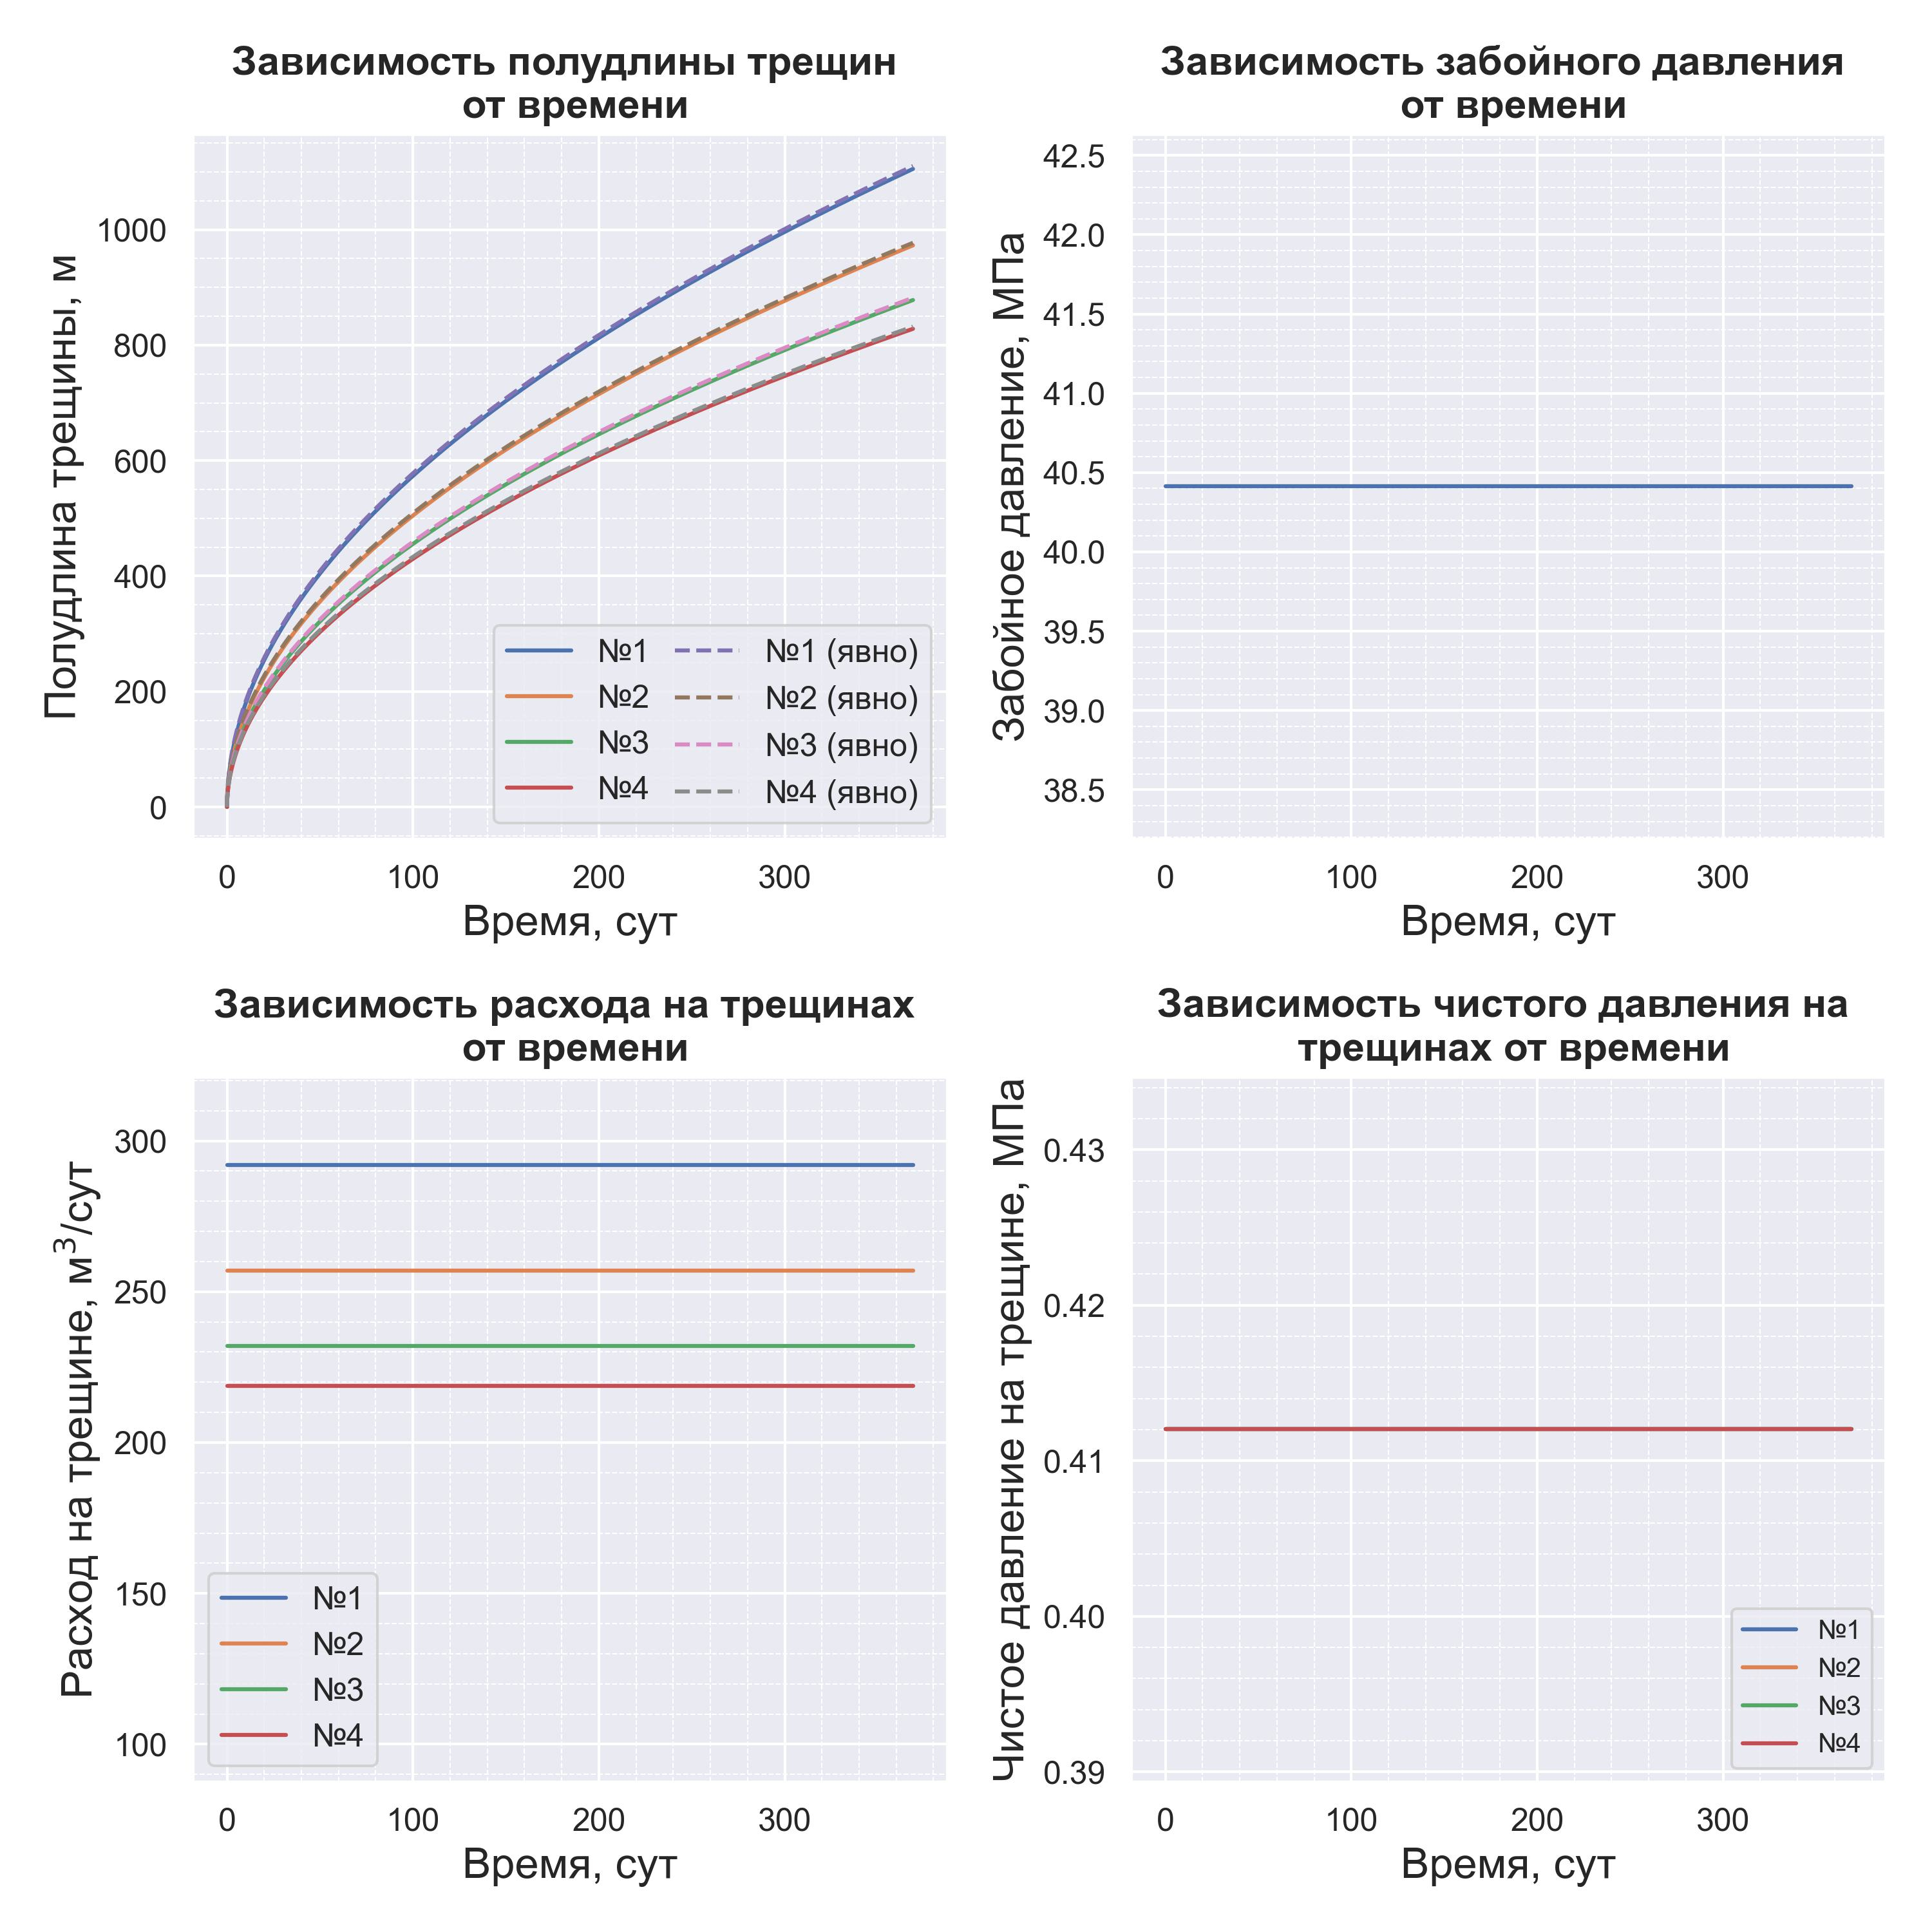
\includegraphics[width=7.5cm]{myimage1.jpg}
\end{textblock*}

\begin{textblock*}{8cm}(8.1cm,1.1cm)
\fbox{\begin{minipage}{10.8em}
\adjustbox{trim={0\width} {0\height} {0.51\width} {0\height},clip}%
  {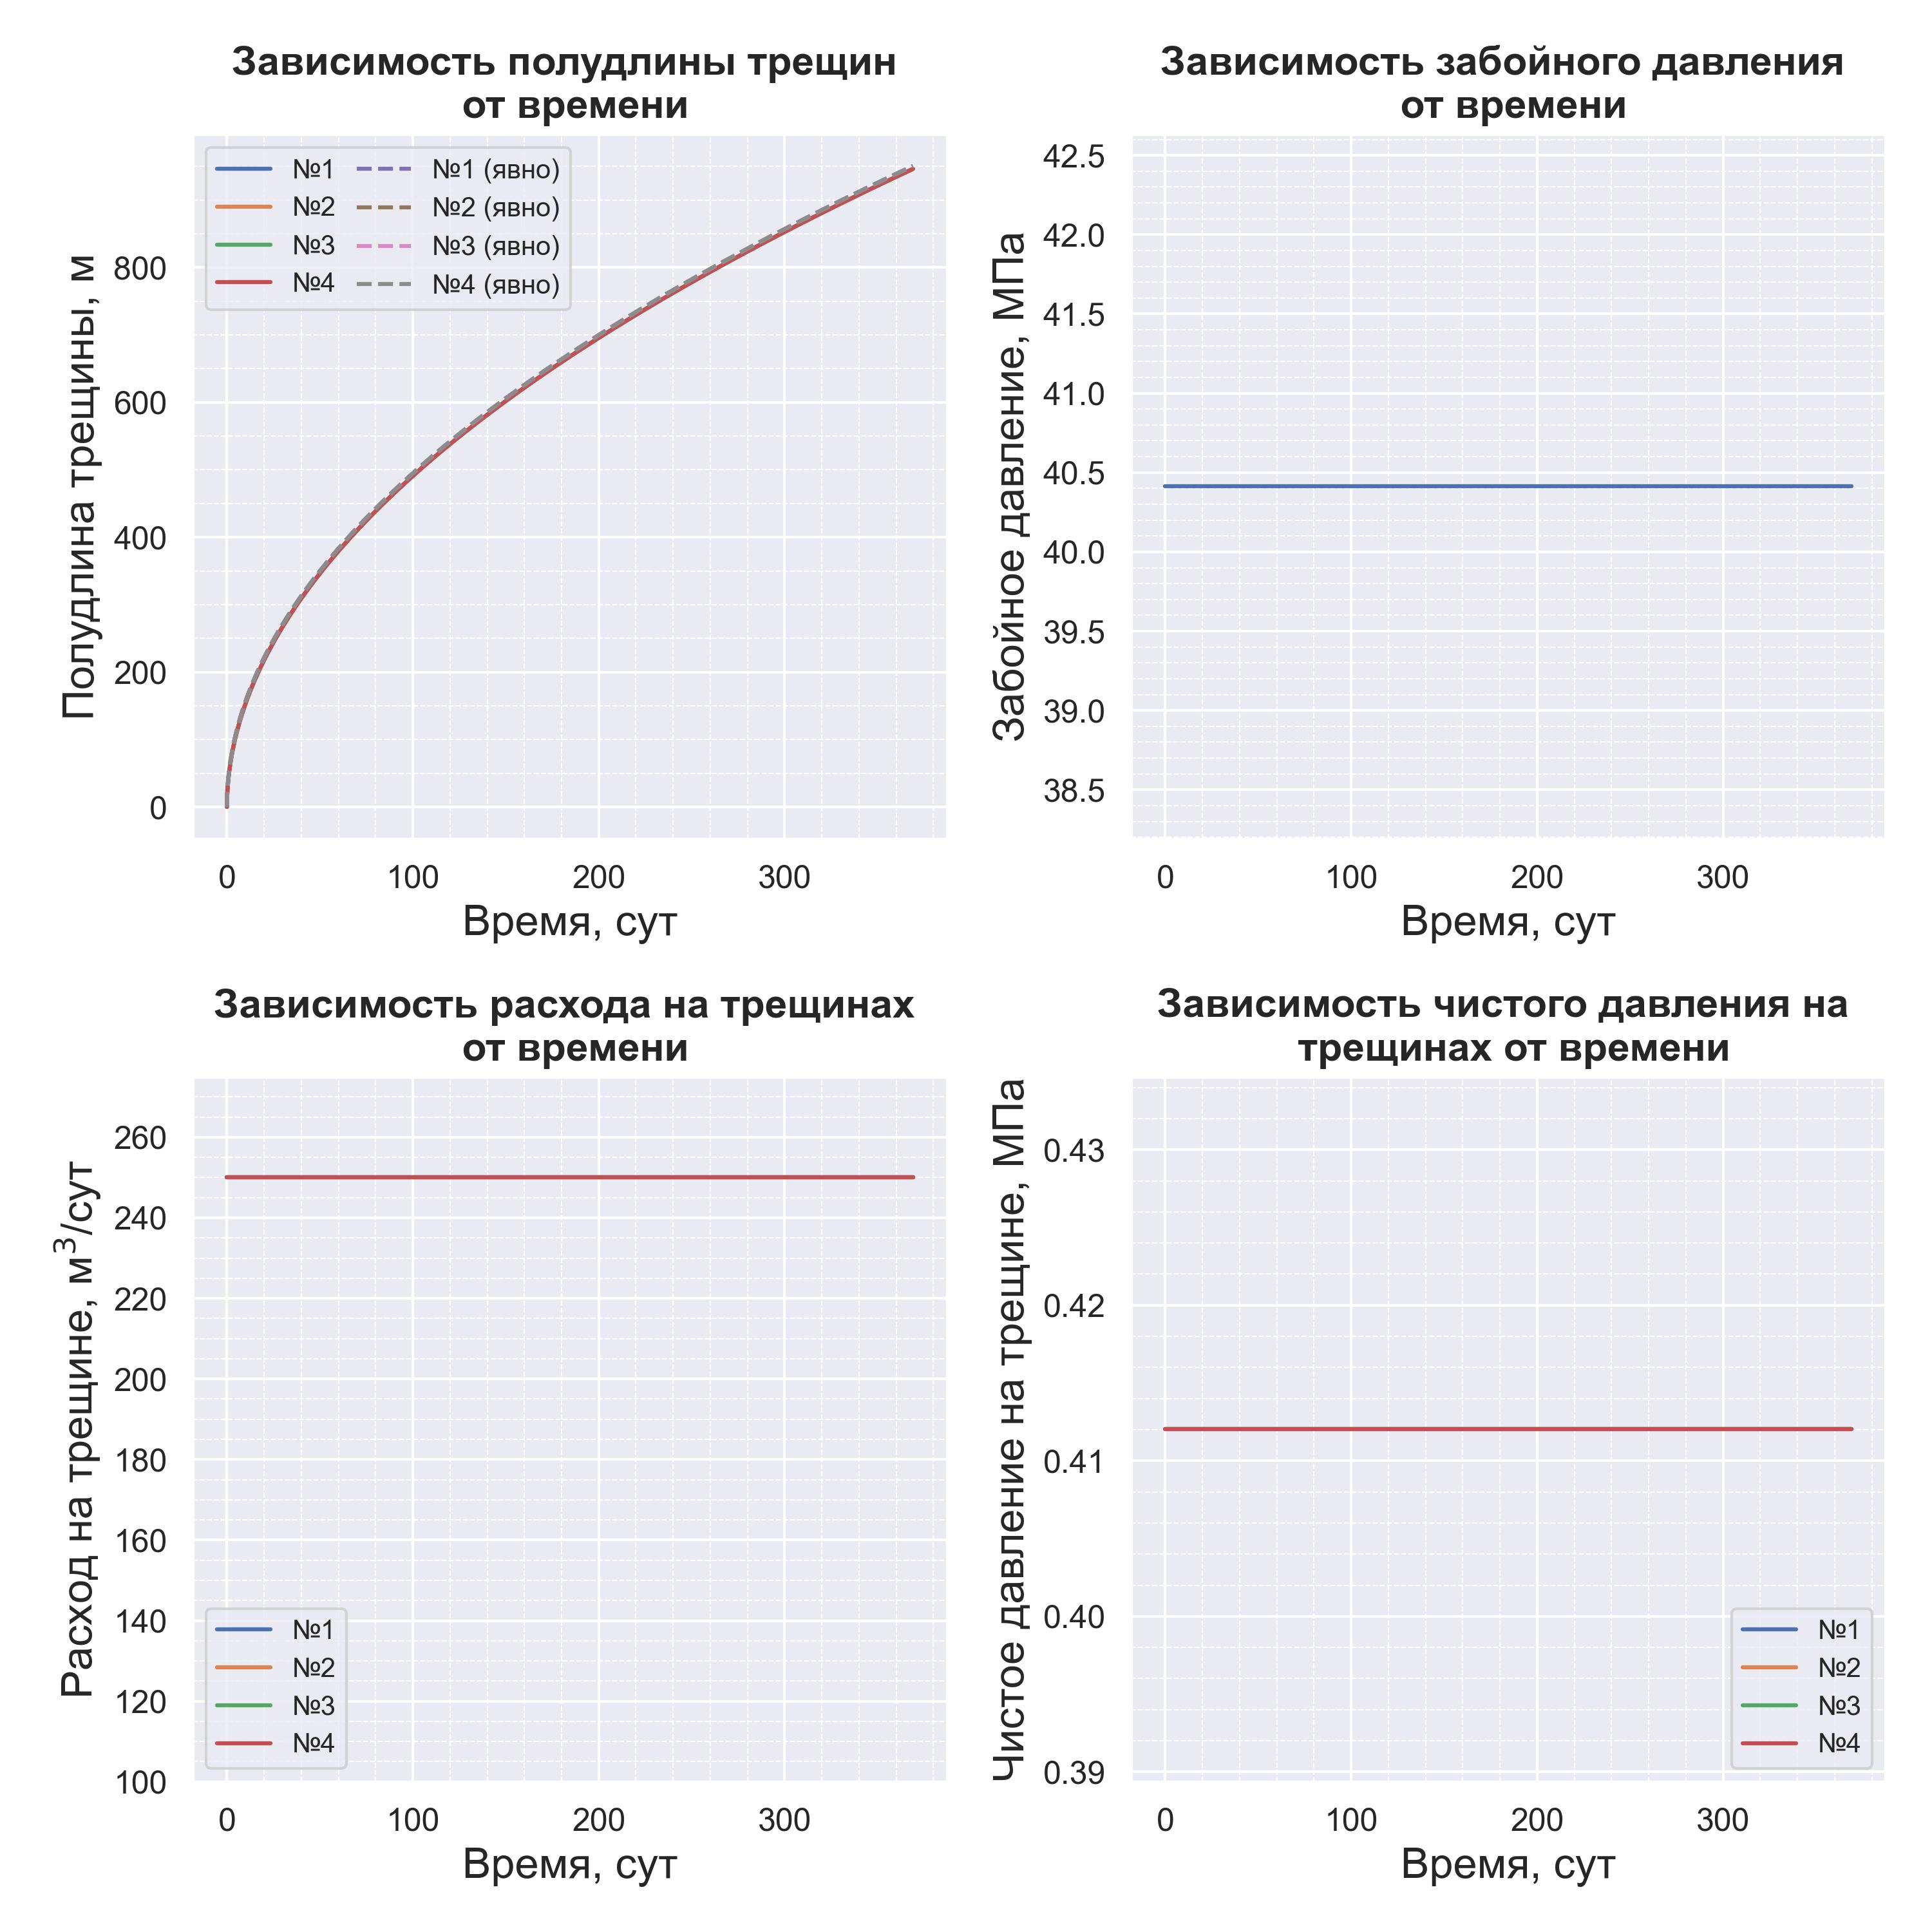
\includegraphics[width=7.7cm]{myimage14.jpg}}
\end{minipage}}
\end{textblock*}

\end{frame}


\begin{frame}
\frametitle{Сравнение роста трещин при одномерных утечках Картера и при двумерных радиальных утечках жидкости}

\begin{textblock*}{8cm}(0.3cm,1.6cm)
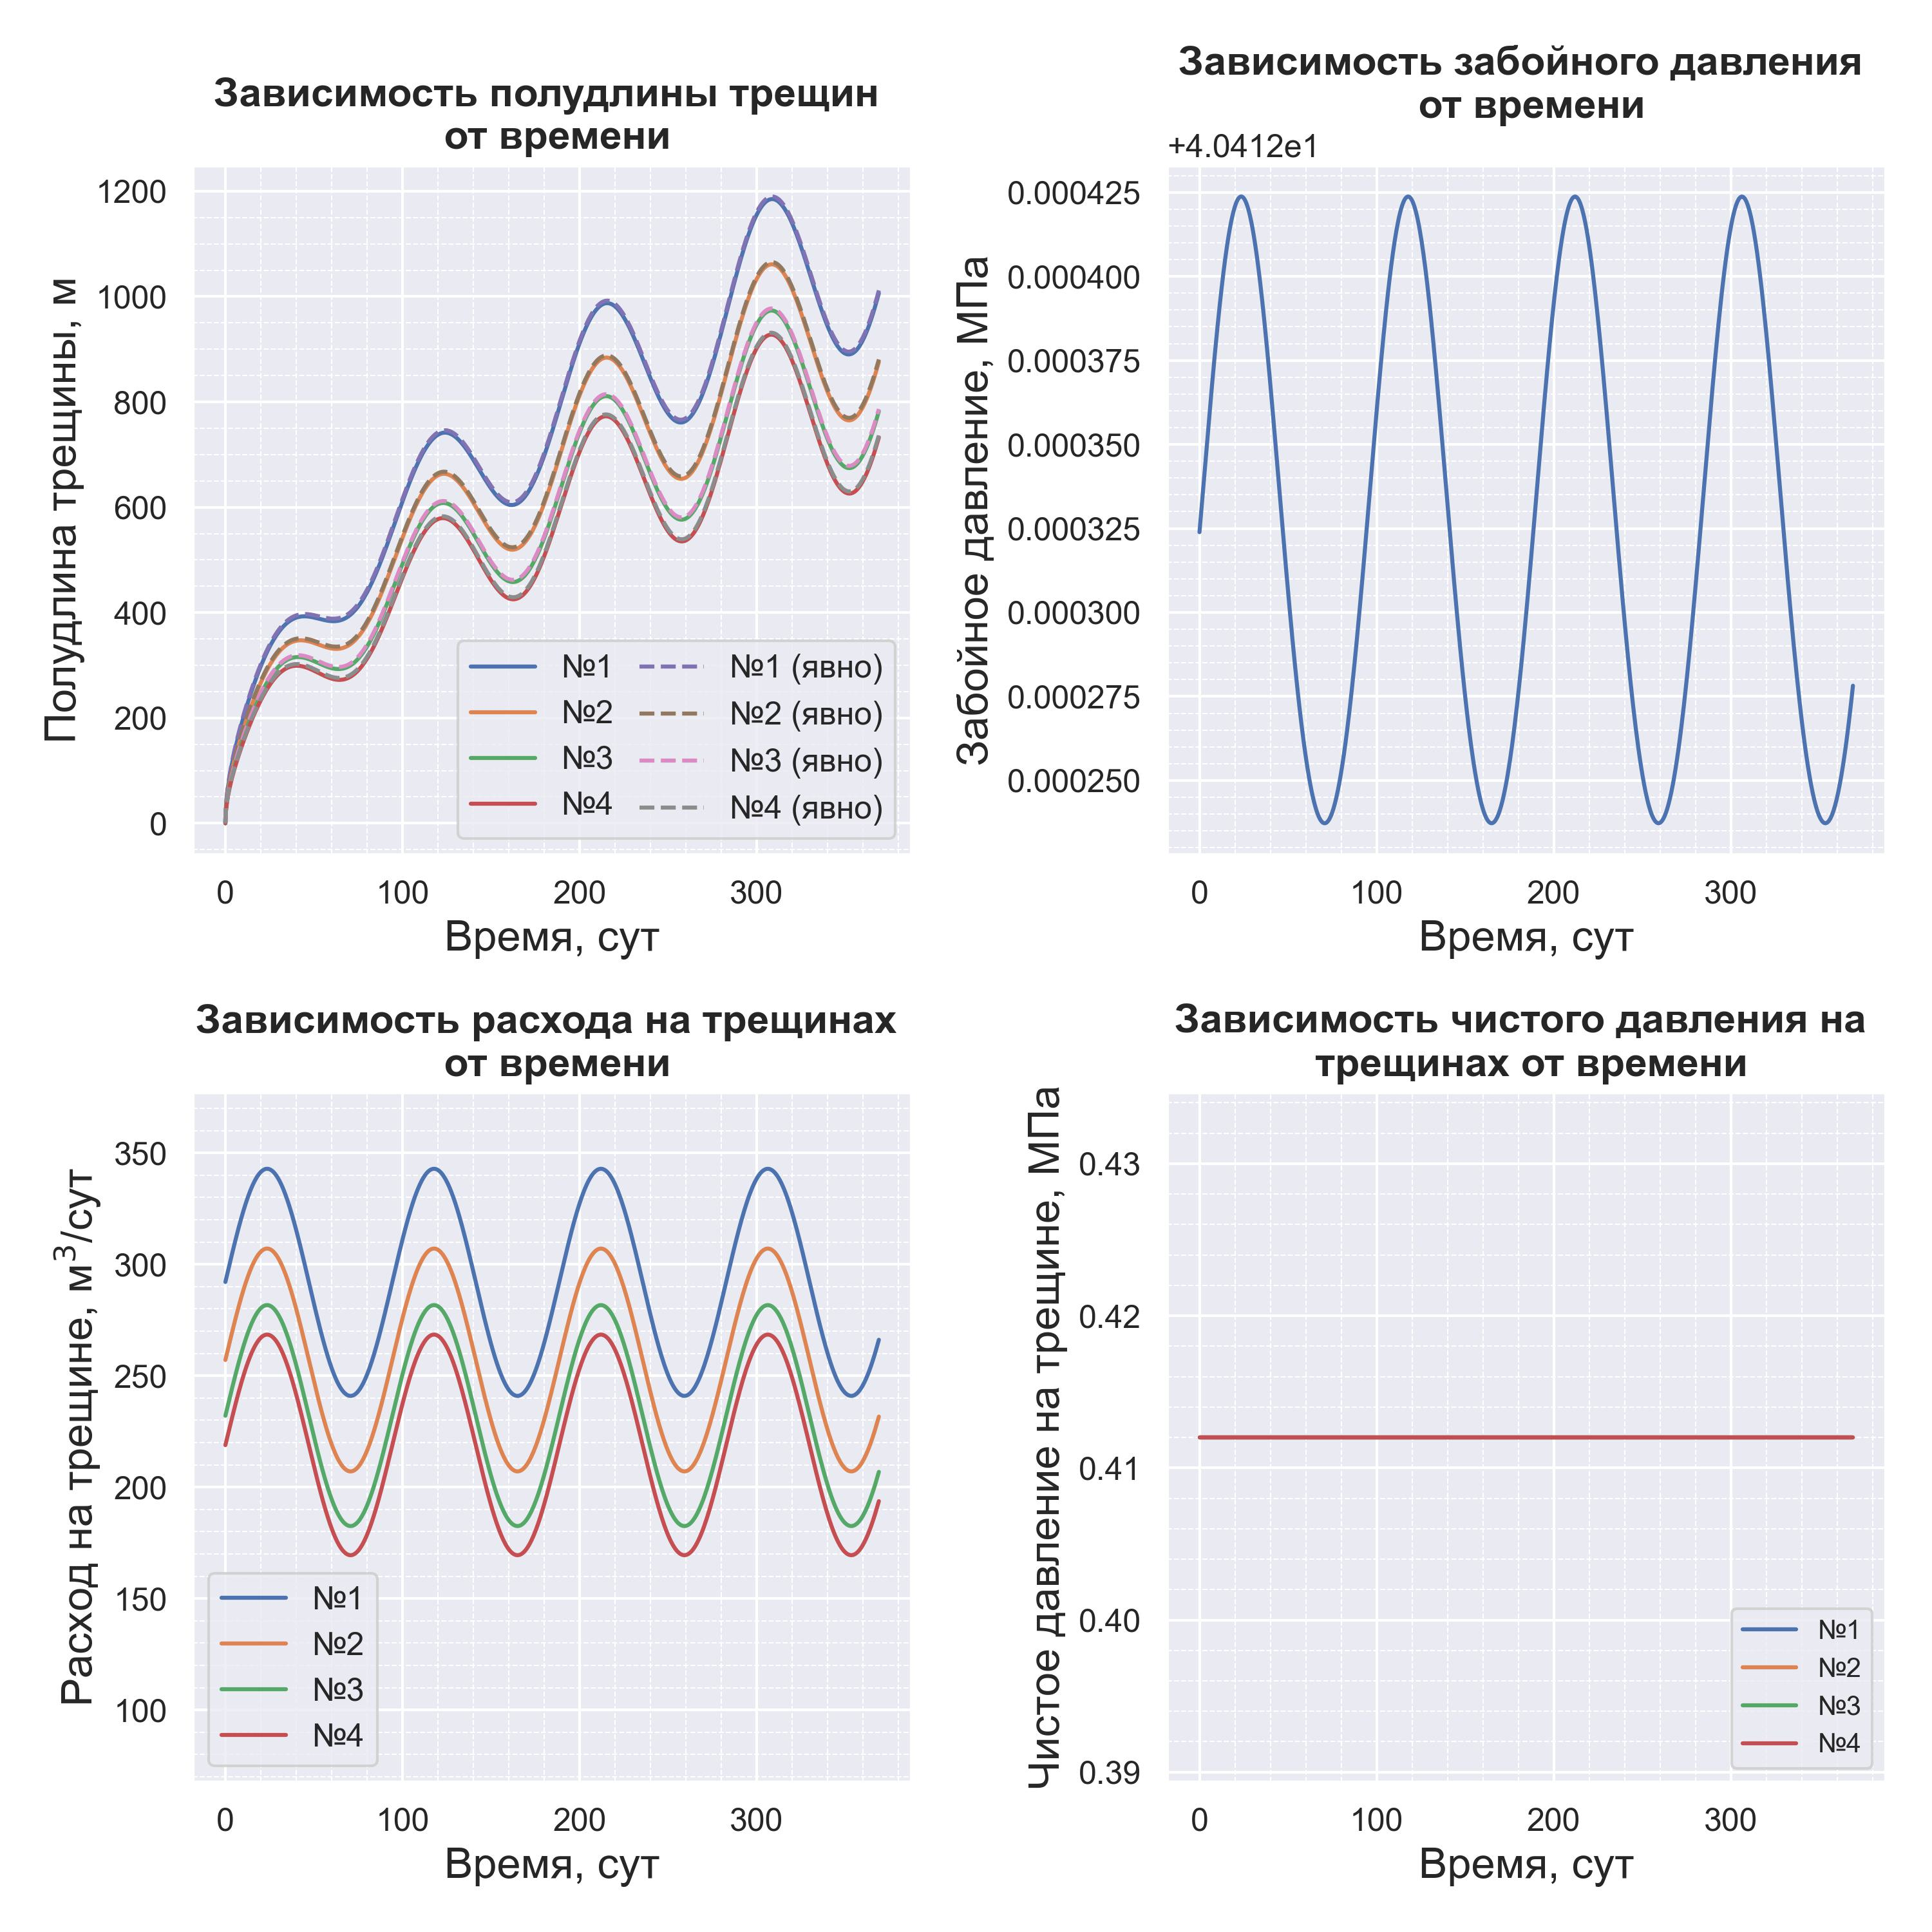
\includegraphics[width=8cm]{myimage3.jpg}
\end{textblock*}

\begin{textblock*}{8cm}(8.3cm,1.6cm)
\adjustbox{trim={0\width} {0\height} {0.51\width} {0\height},clip}%
  {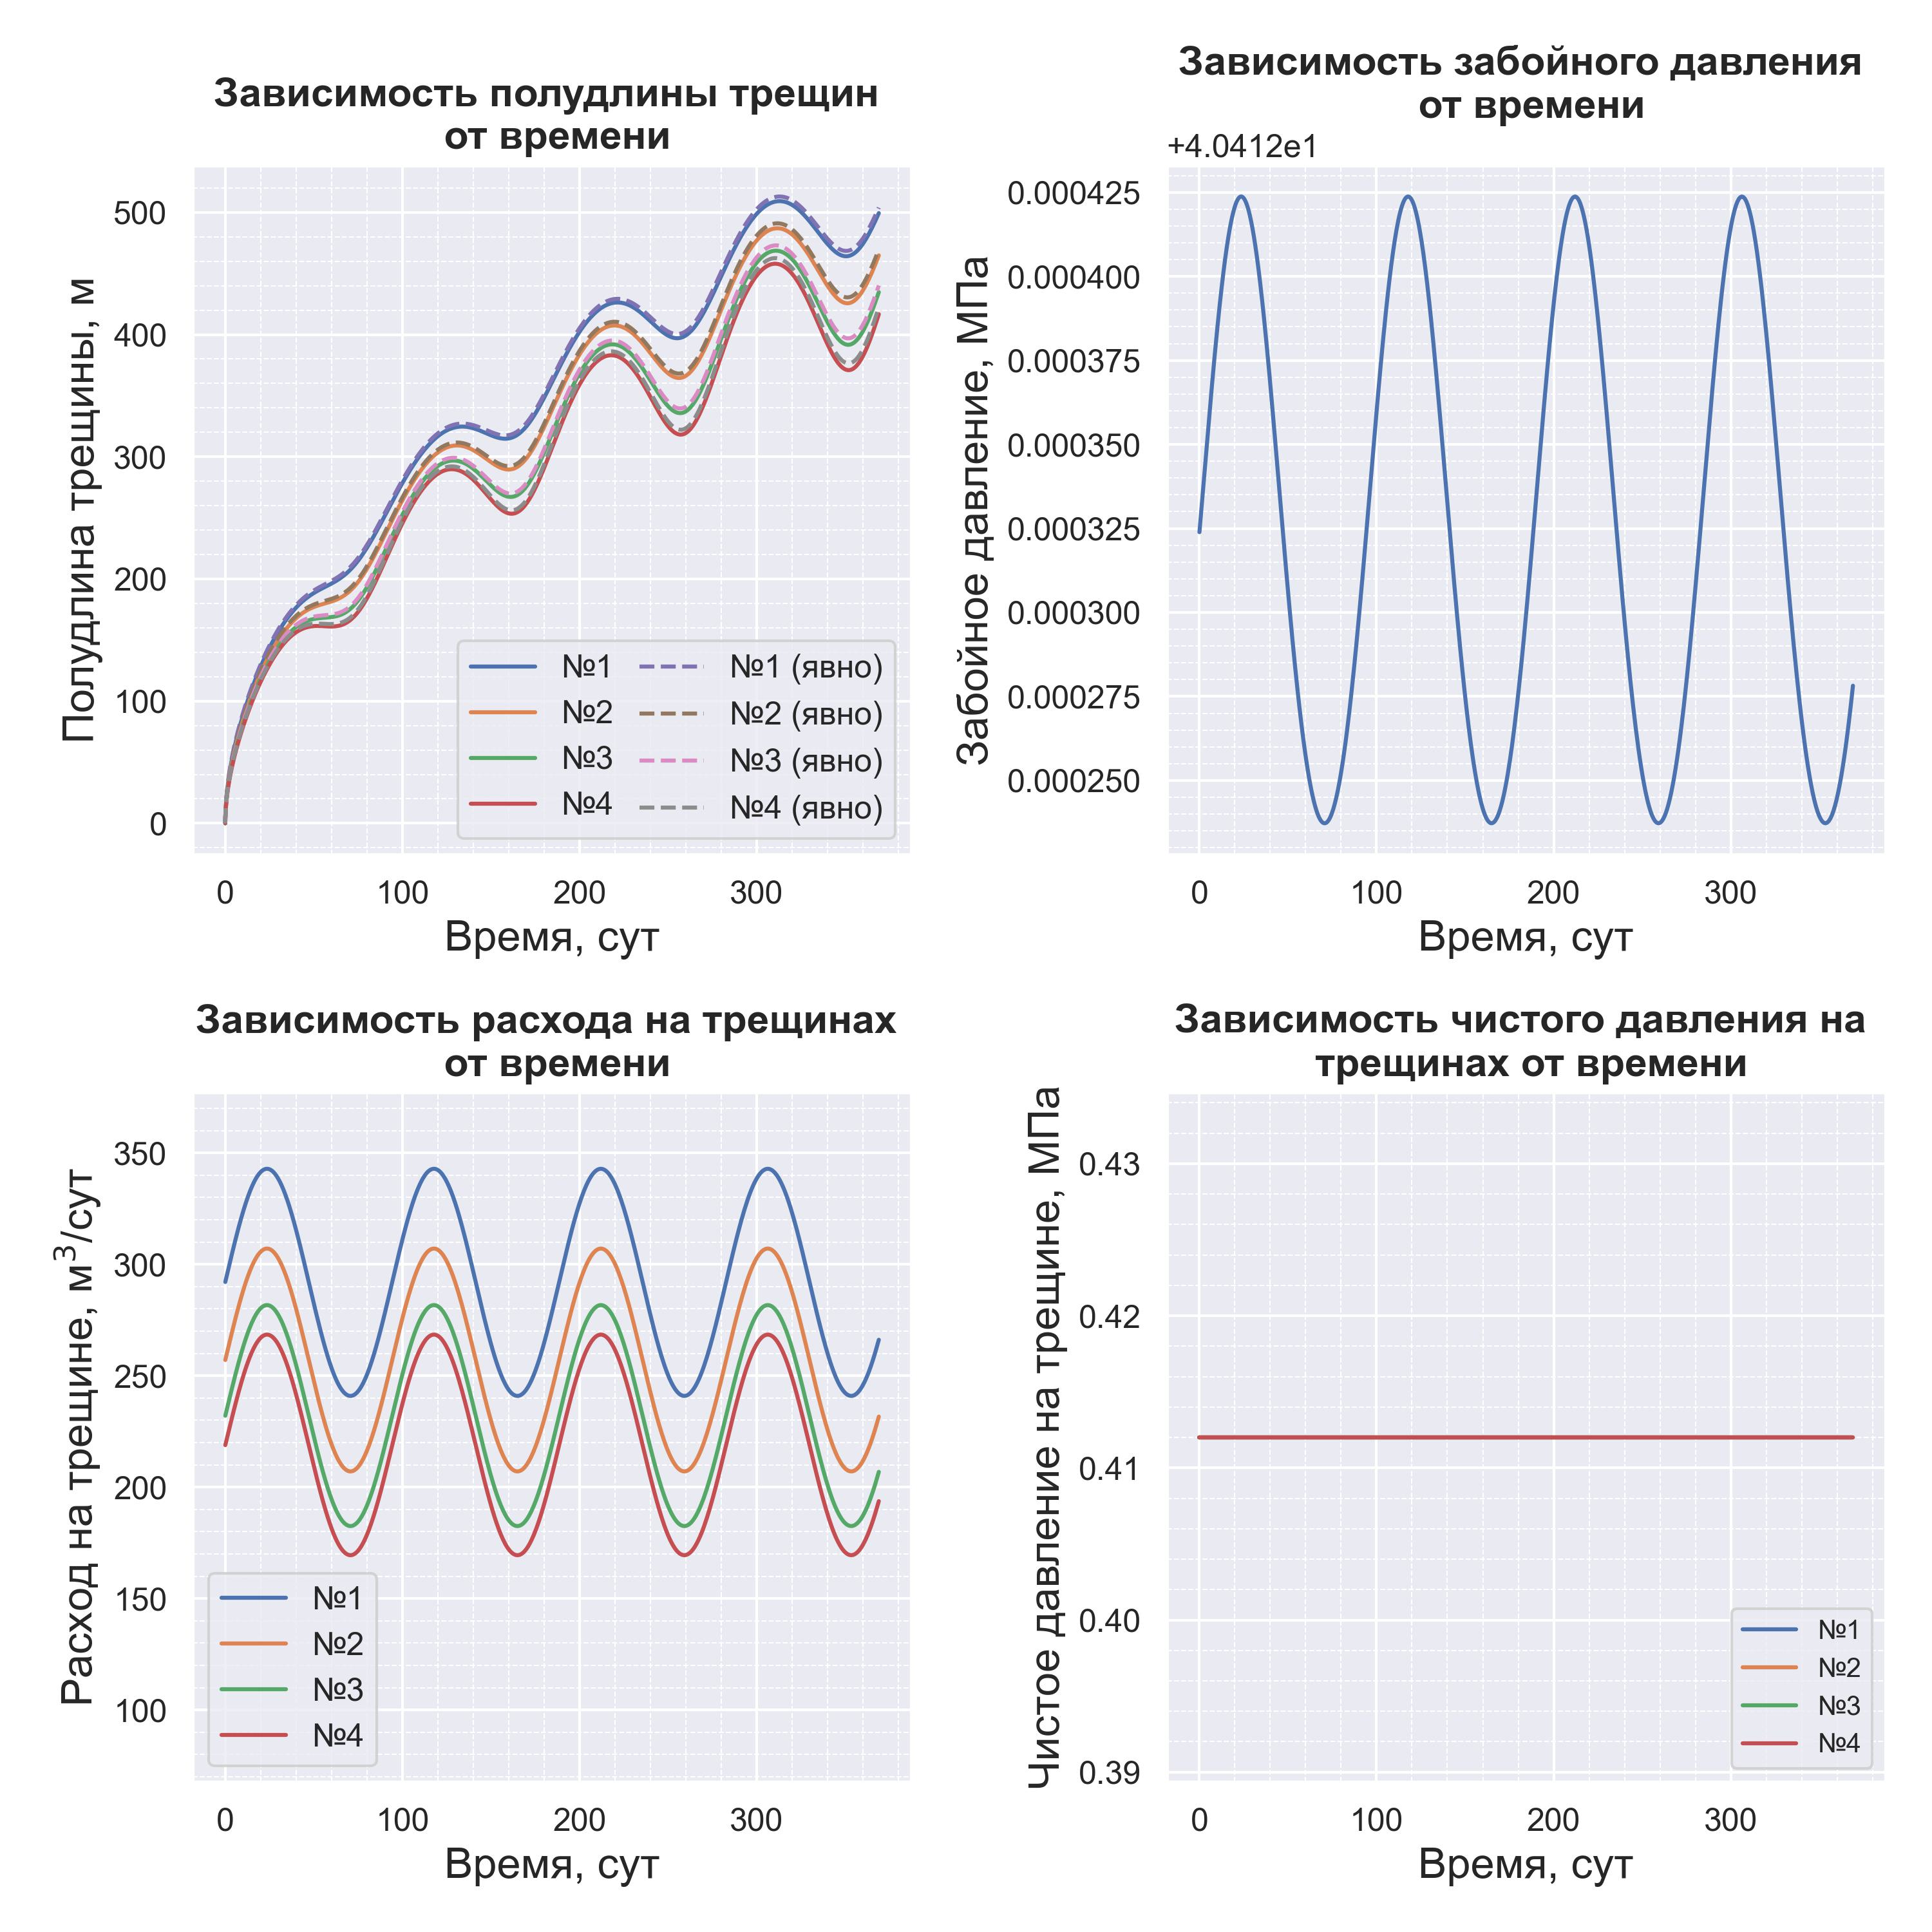
\includegraphics[width=8cm]{myimage4.jpg}}
\end{textblock*}

\end{frame}


\begin{frame}
\frametitle{Результаты при линейном уменьшении расхода жидкости на забое скважины}

\begin{textblock*}{8cm}(0.3cm,1.6cm)
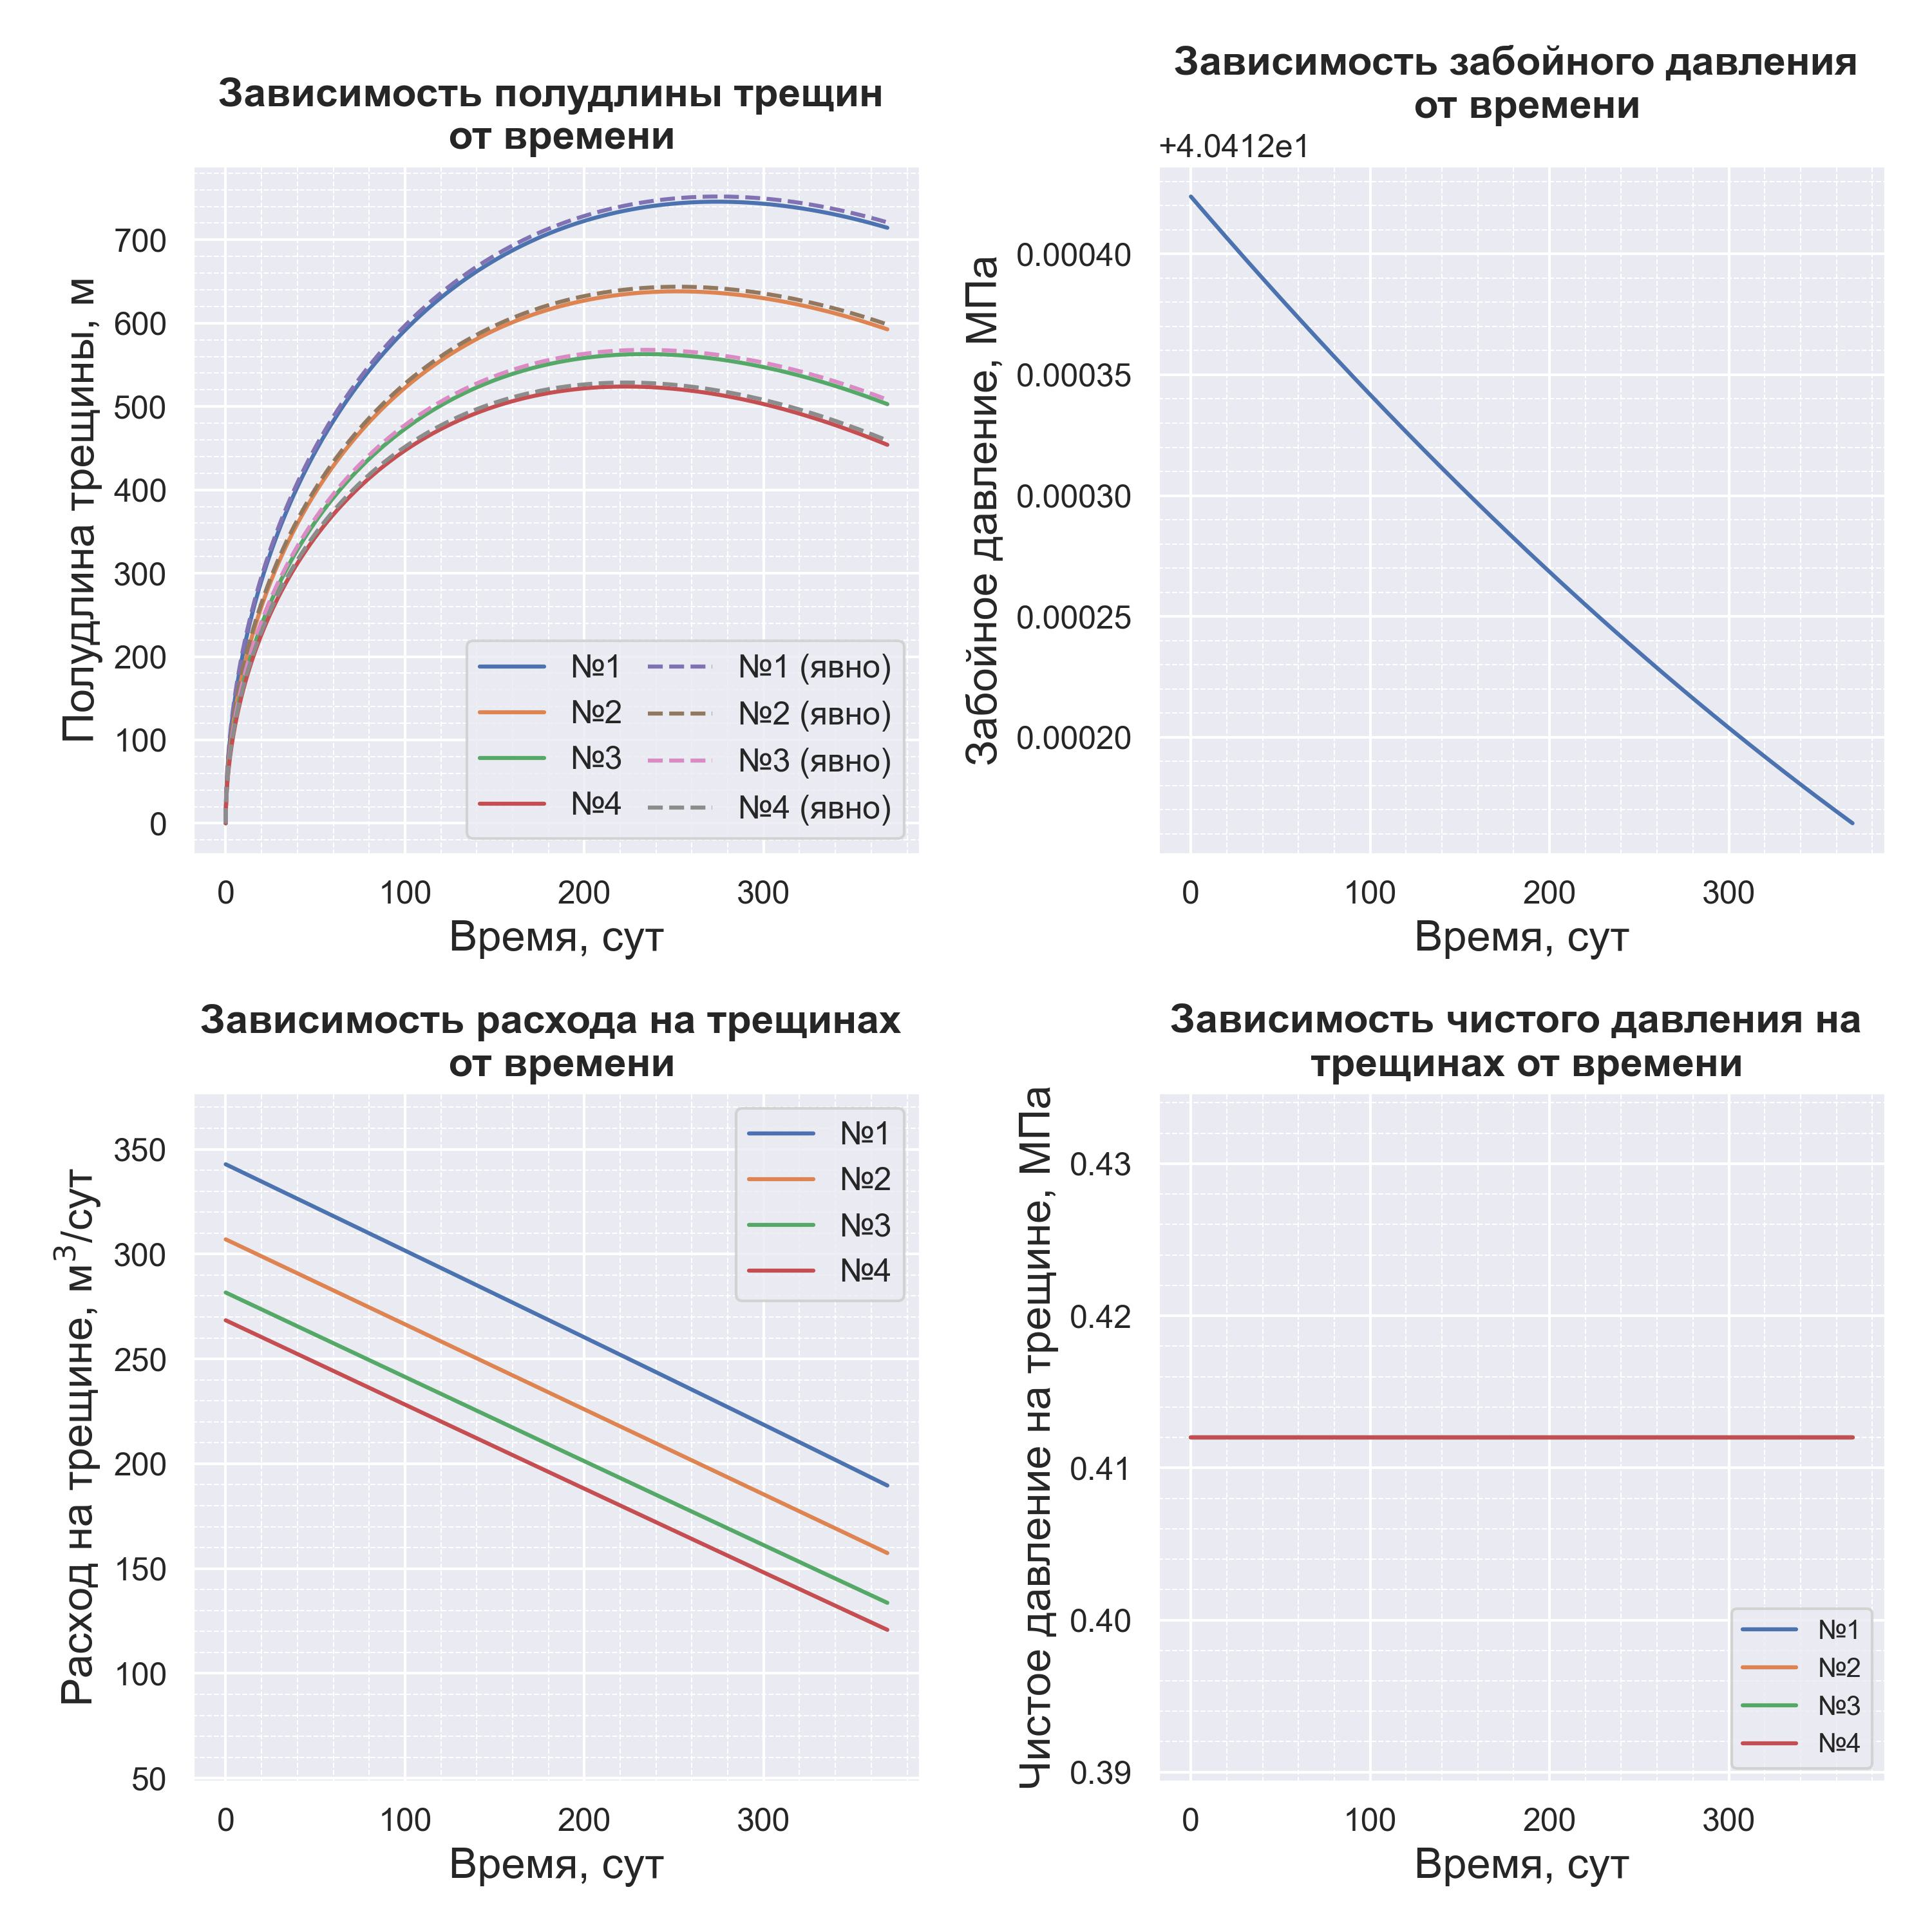
\includegraphics[width=8cm]{myimage5.jpg}
\end{textblock*}

\begin{textblock*}{8cm}(8.3cm,1.6cm)
\adjustbox{trim={0\width} {0\height} {0.51\width} {0\height},clip}%
  {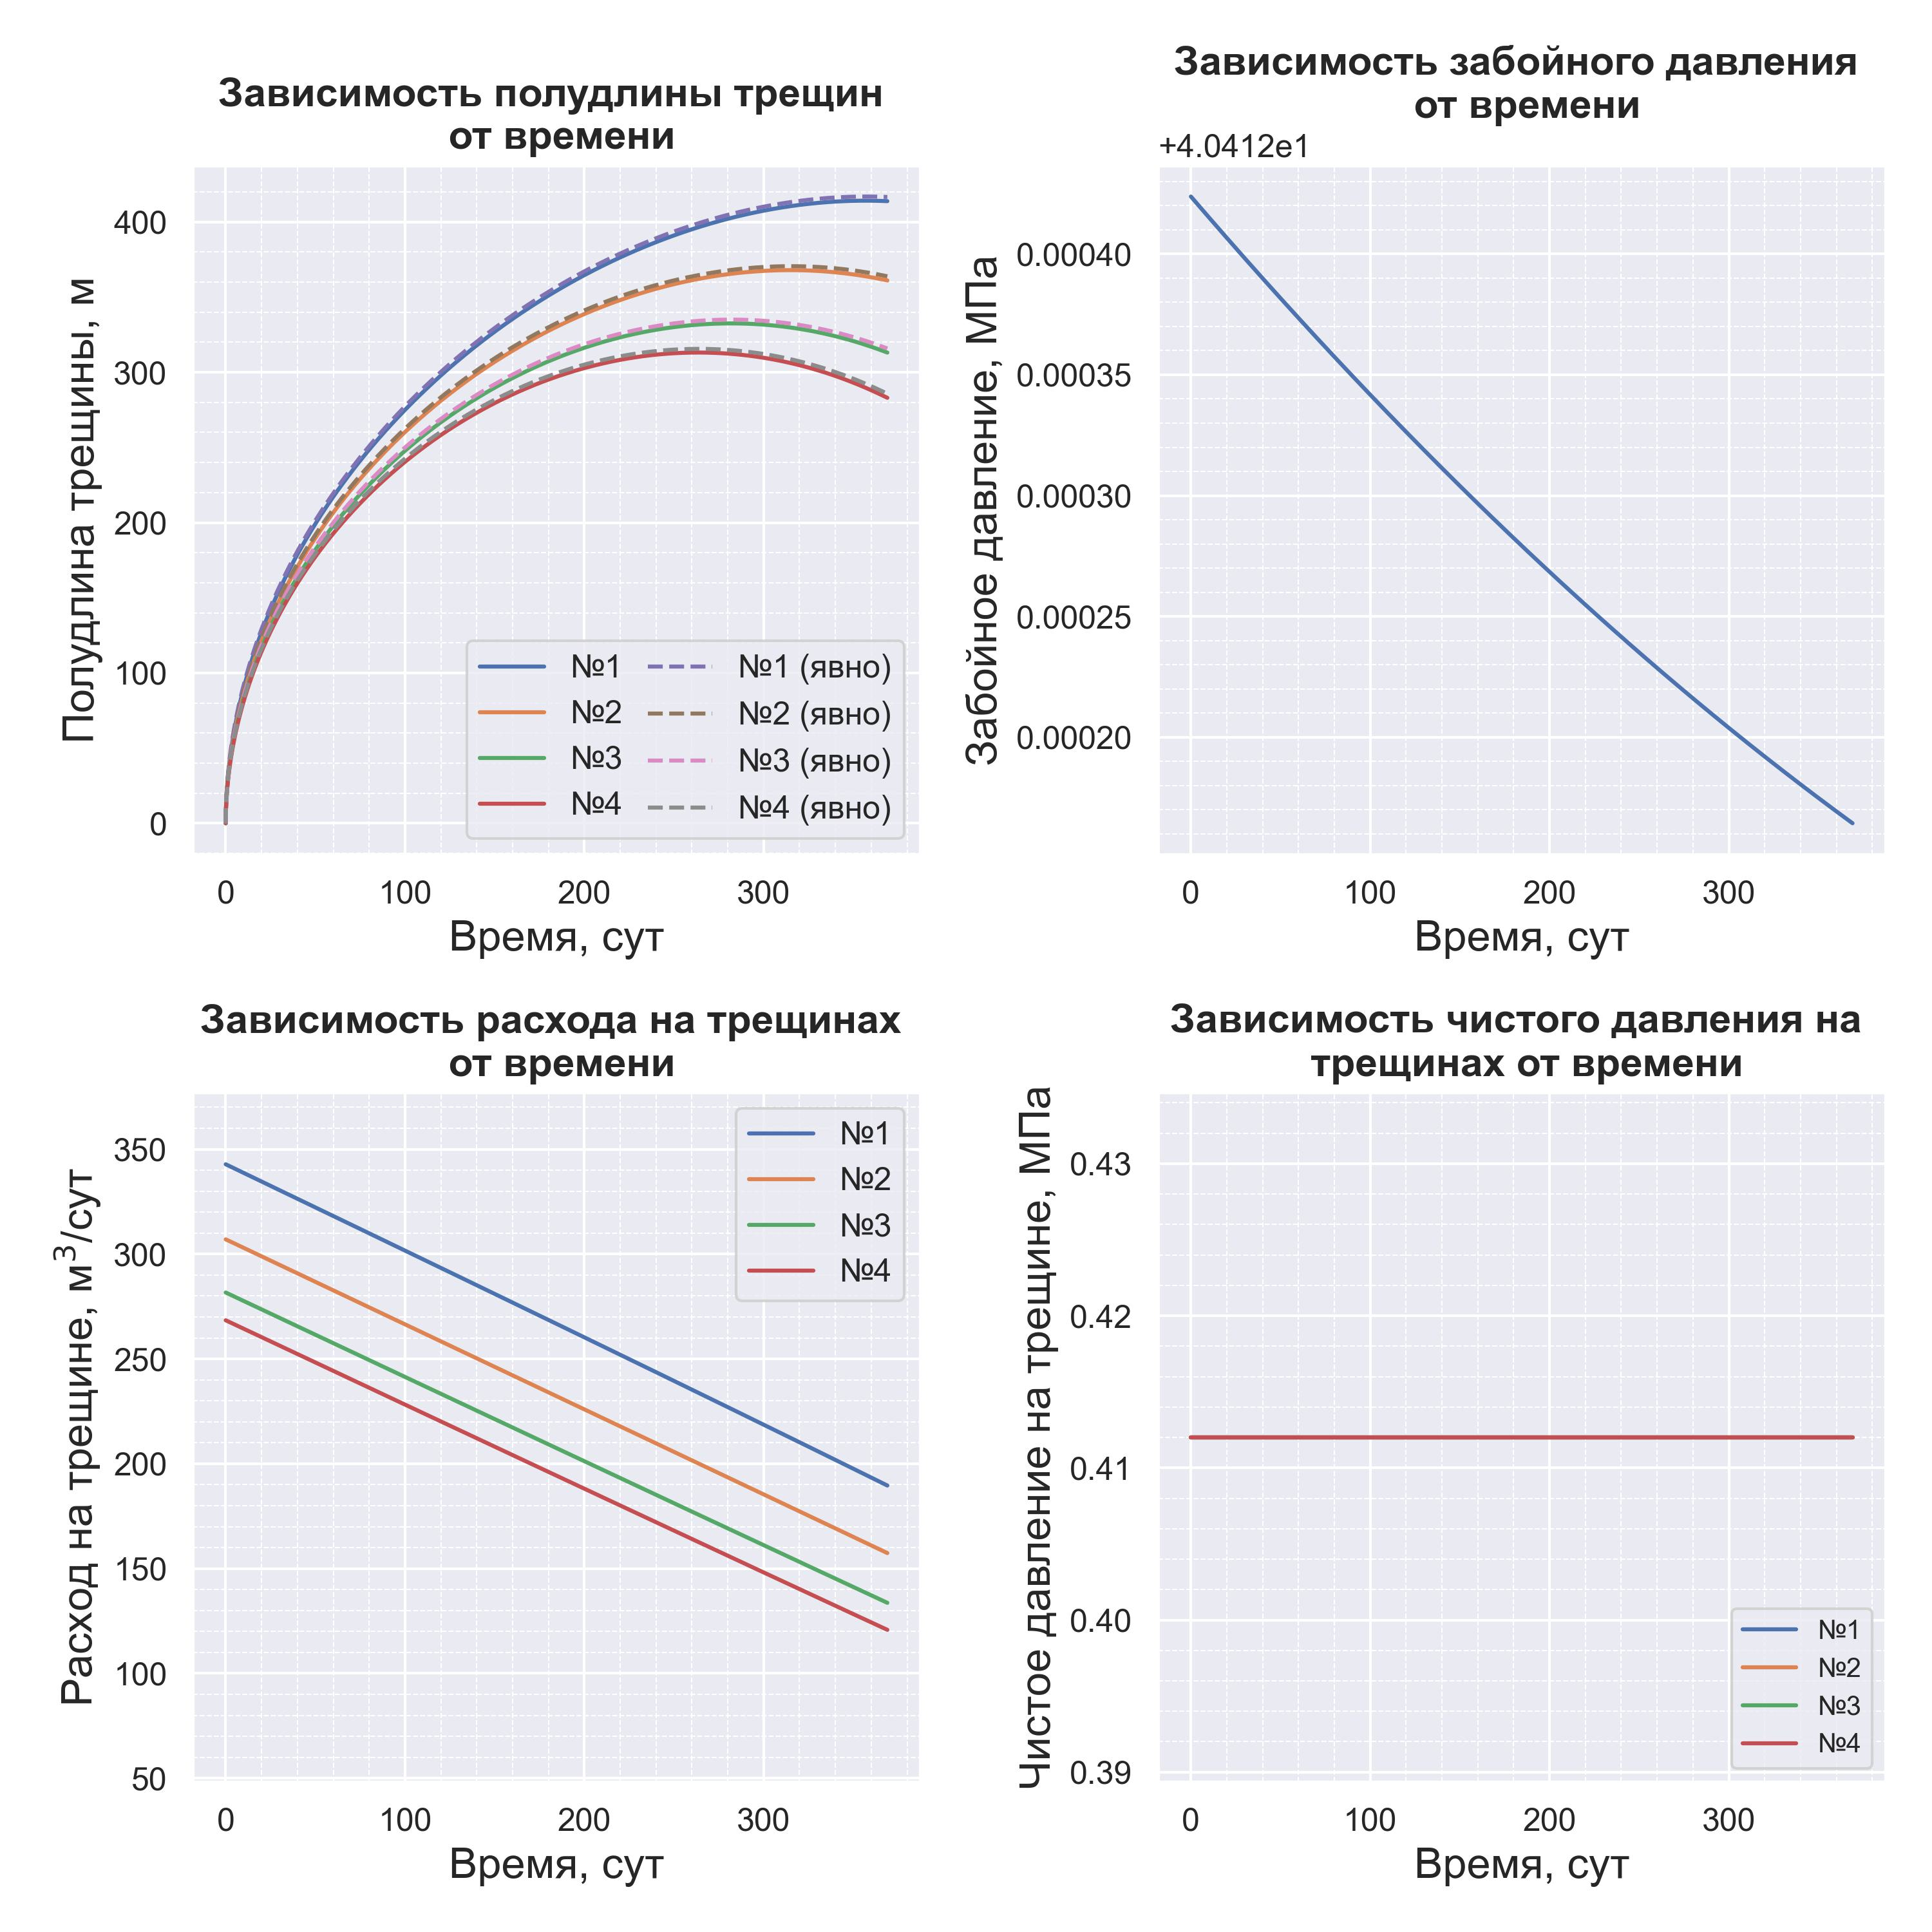
\includegraphics[width=8cm]{myimage6.jpg}}
\end{textblock*}

\end{frame}


\begin{frame}
\frametitle{Результаты при ухудшении качества перфораций на одной из трещин}

\begin{textblock*}{8cm}(0.3cm,1.6cm)
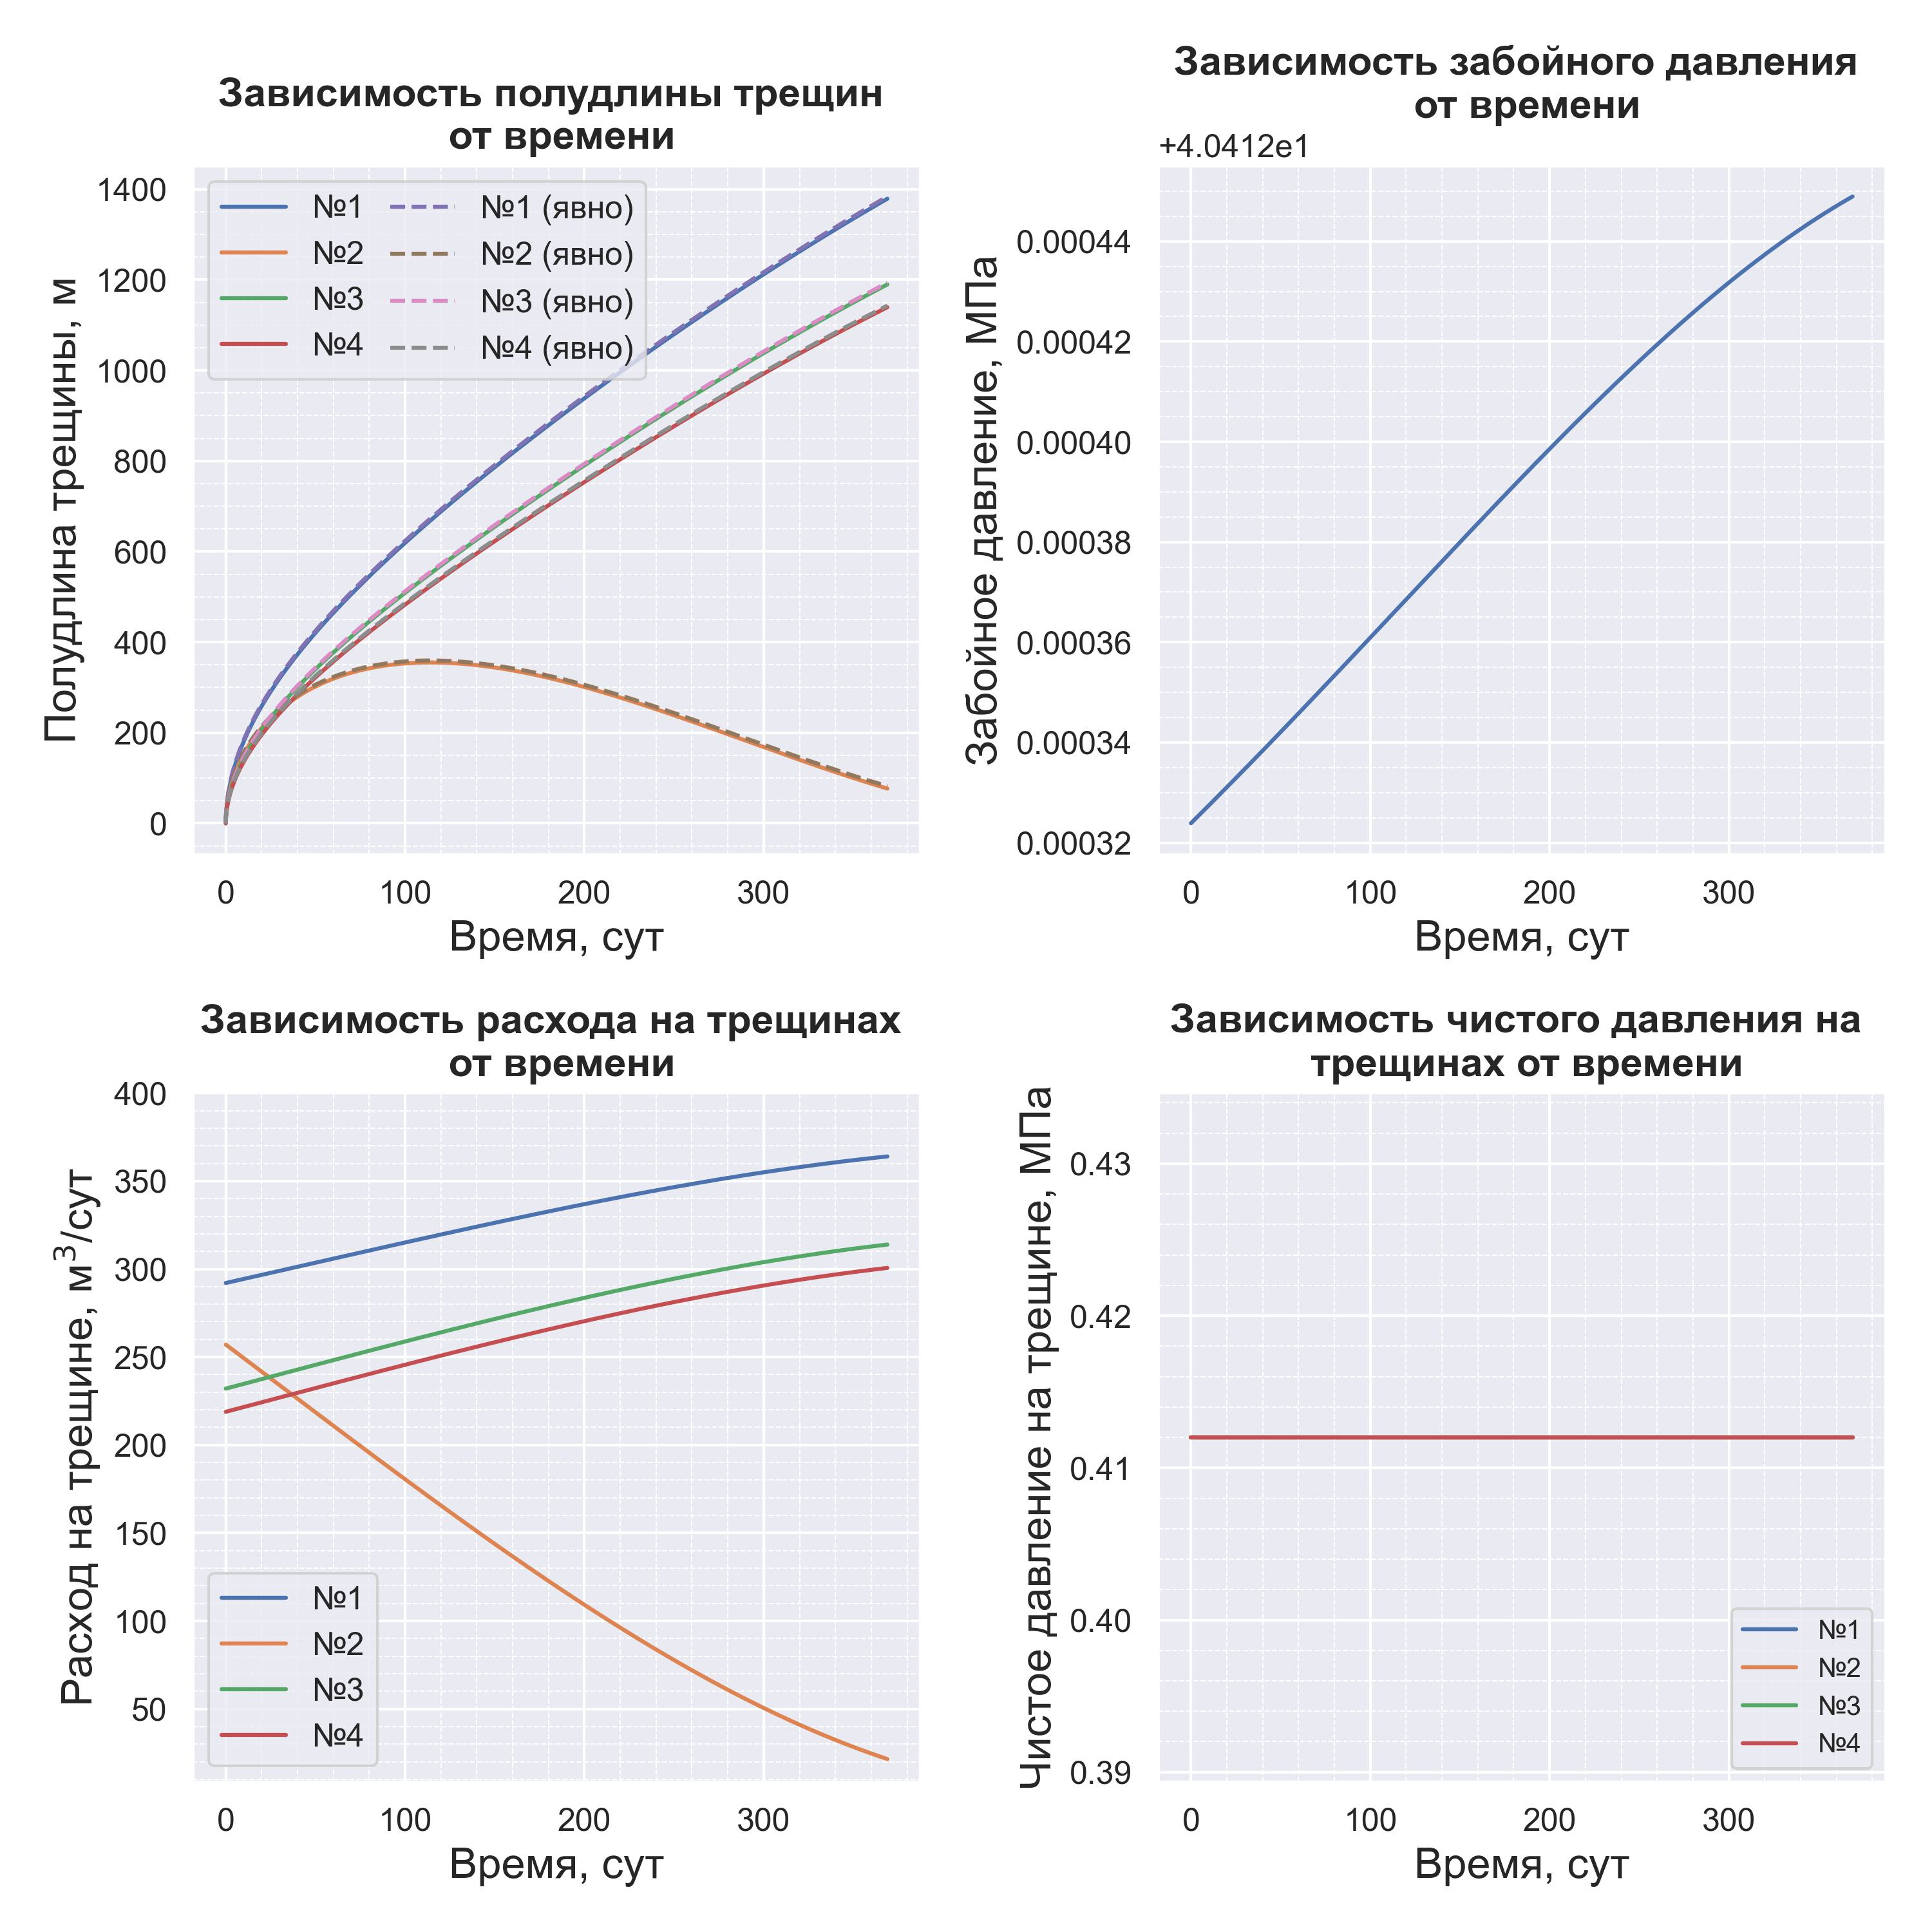
\includegraphics[width=8cm]{myimage7.jpg}
\end{textblock*}

\begin{textblock*}{8cm}(8.3cm,1.6cm)
\adjustbox{trim={0\width} {0\height} {0.51\width} {0\height},clip}%
  {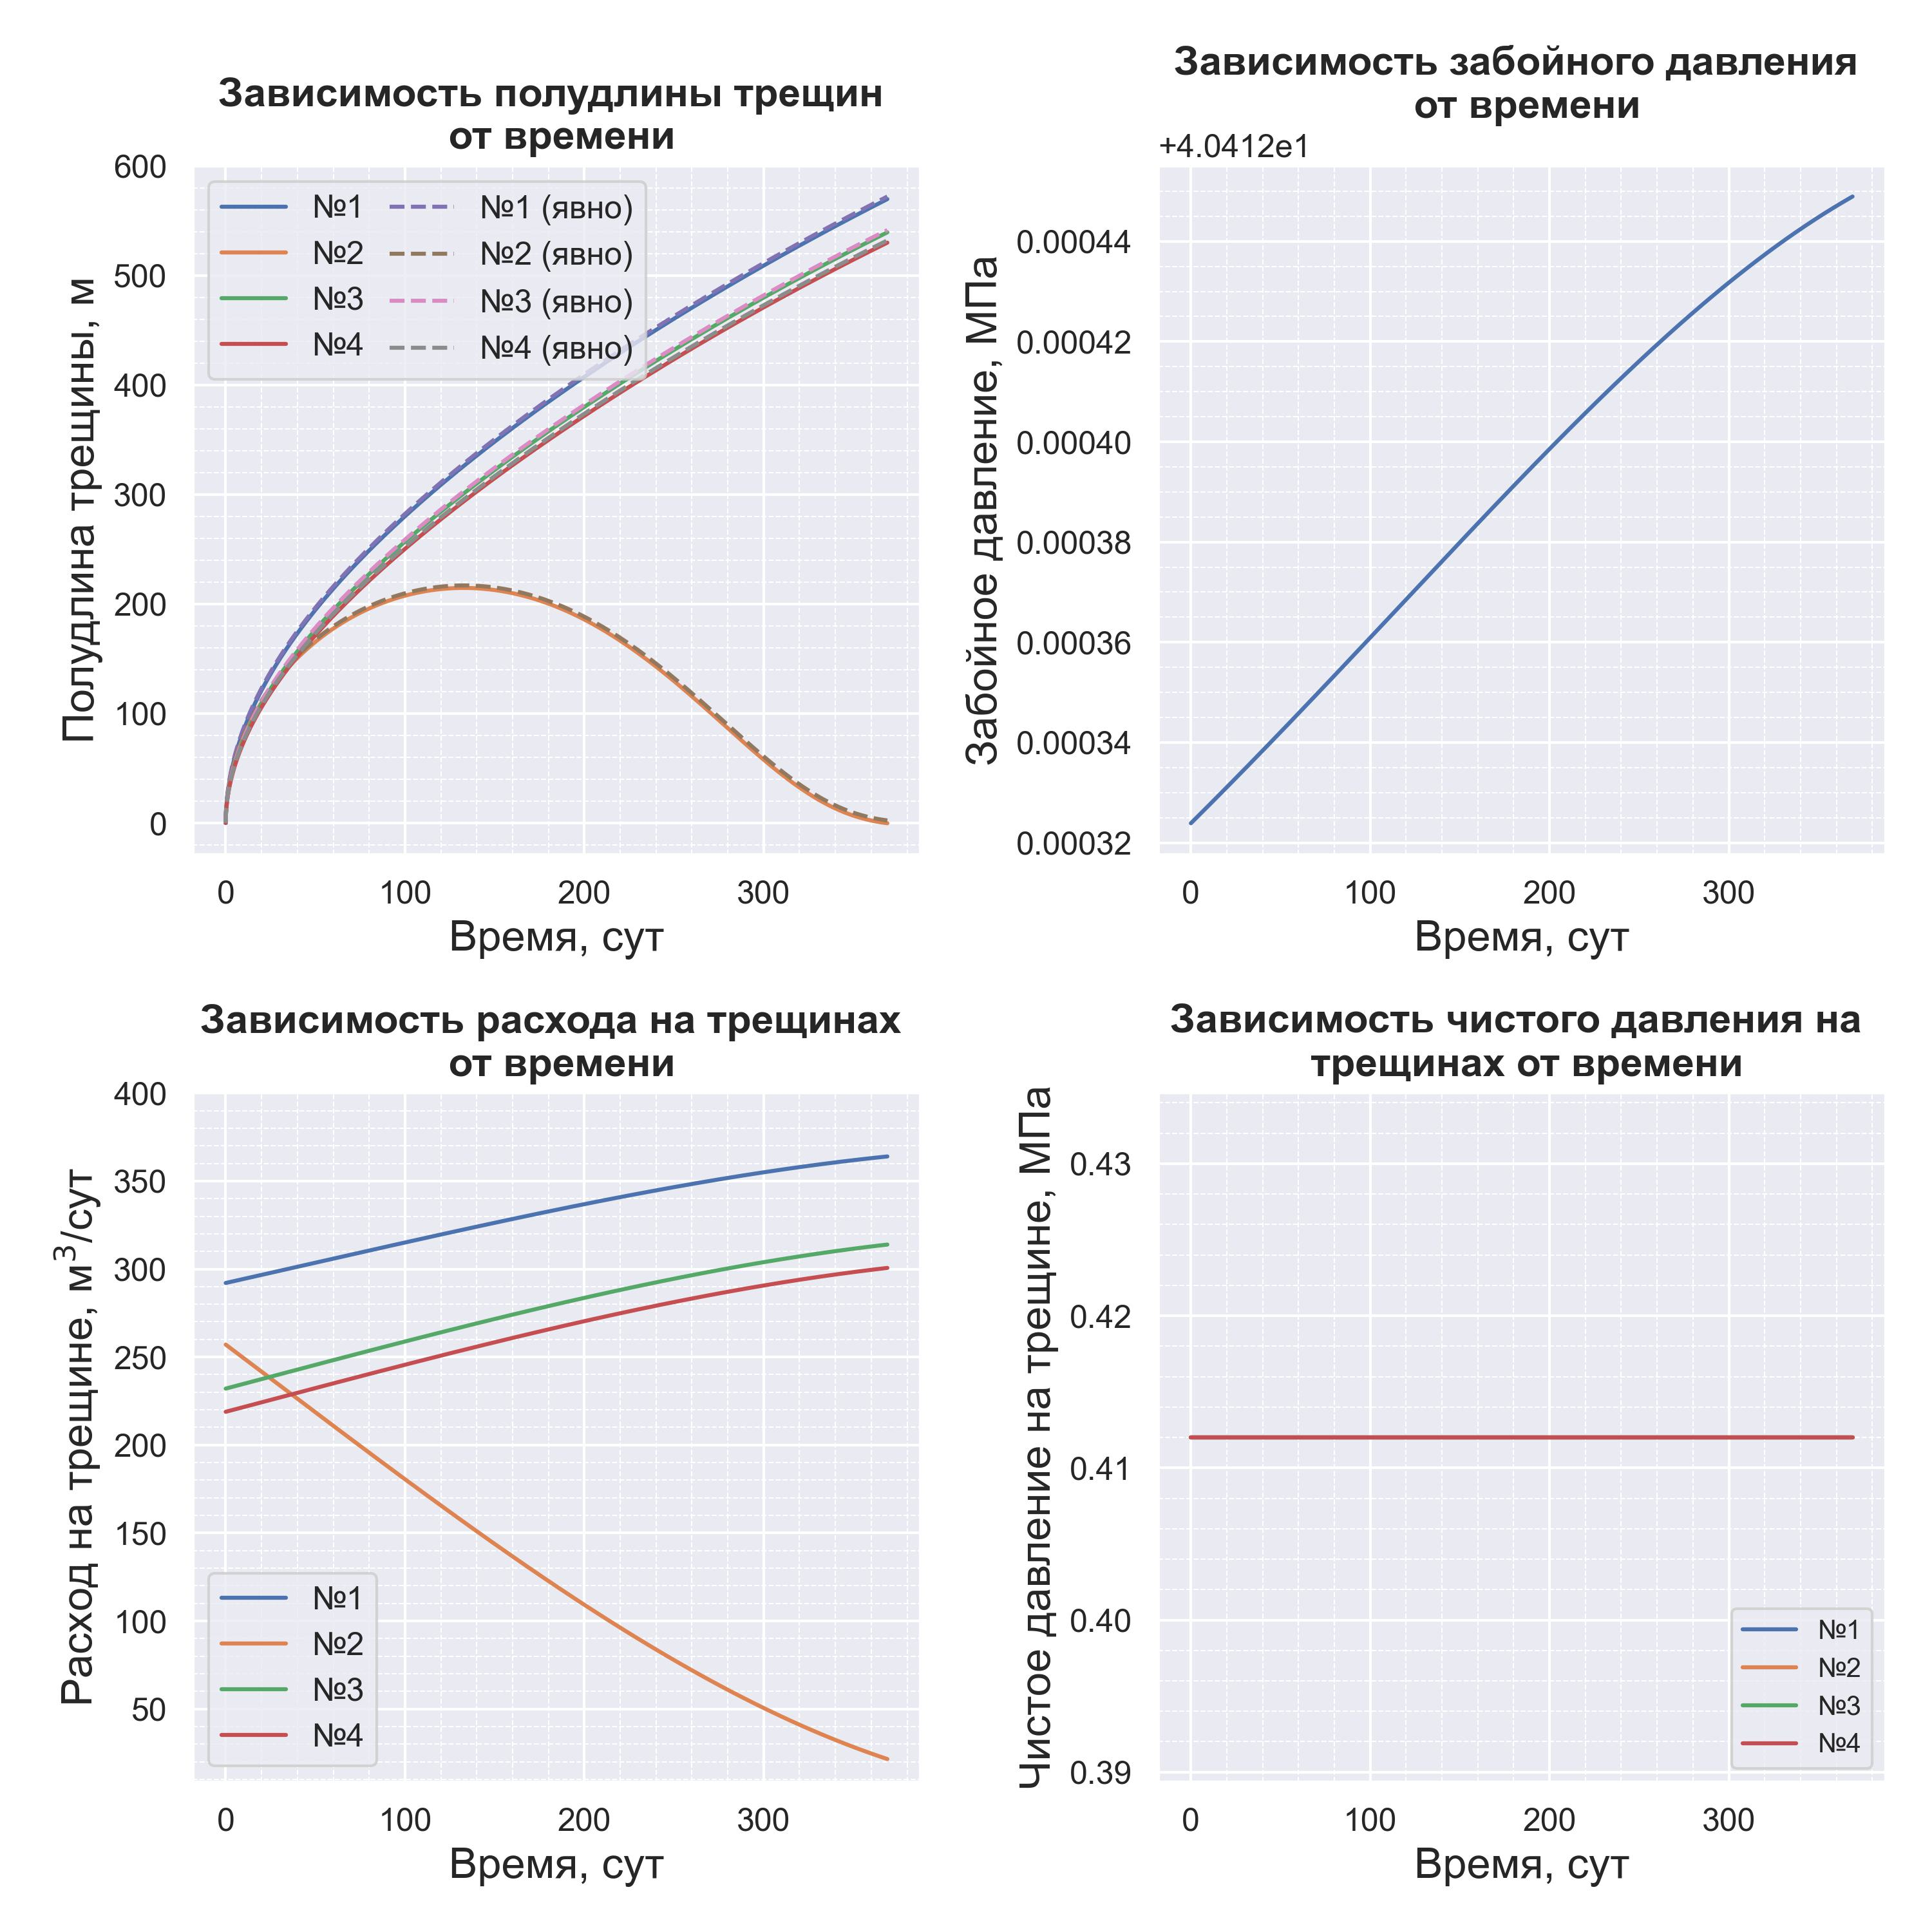
\includegraphics[width=8cm]{myimage8.jpg}}
\end{textblock*}

\end{frame}


\begin{frame}
\frametitle{Результаты при уменьшении горизонтальных напряжений в пласте}

\begin{textblock*}{8cm}(0.3cm,1.6cm)
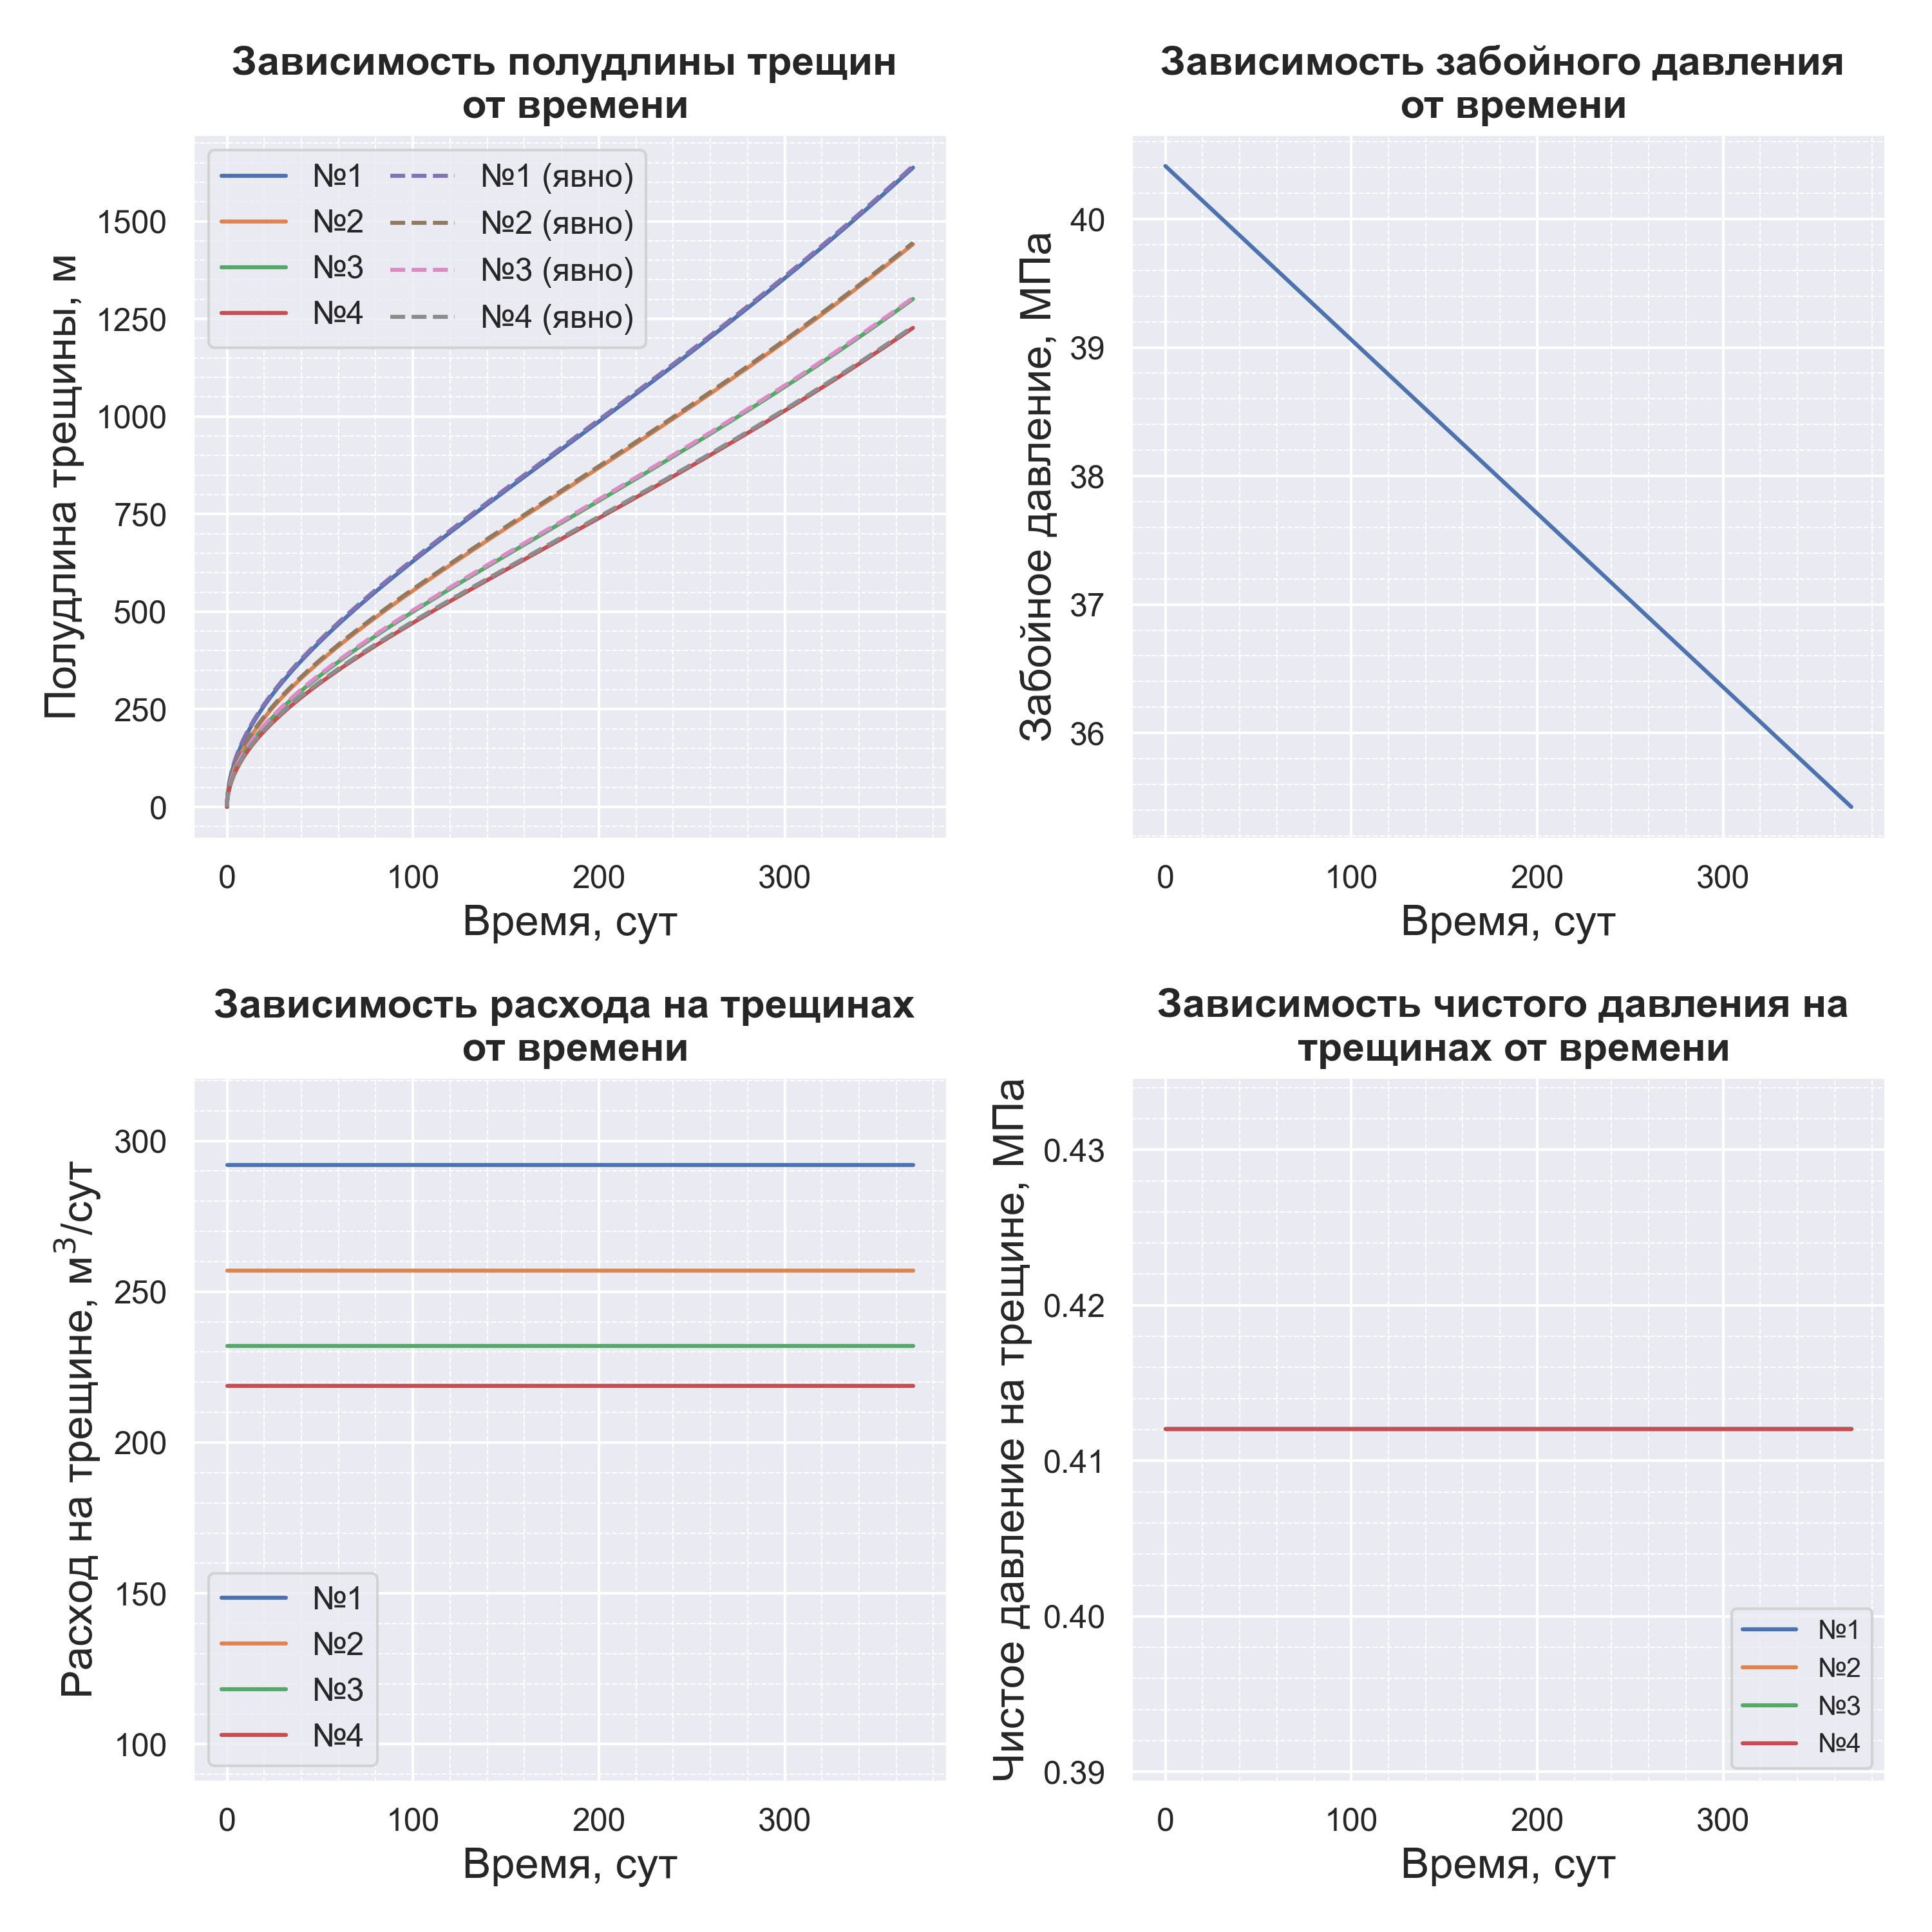
\includegraphics[width=8cm]{myimage11.jpg}
\end{textblock*}

\begin{textblock*}{8cm}(8.3cm,1.6cm)
\adjustbox{trim={0\width} {0\height} {0.51\width} {0\height},clip}%
  {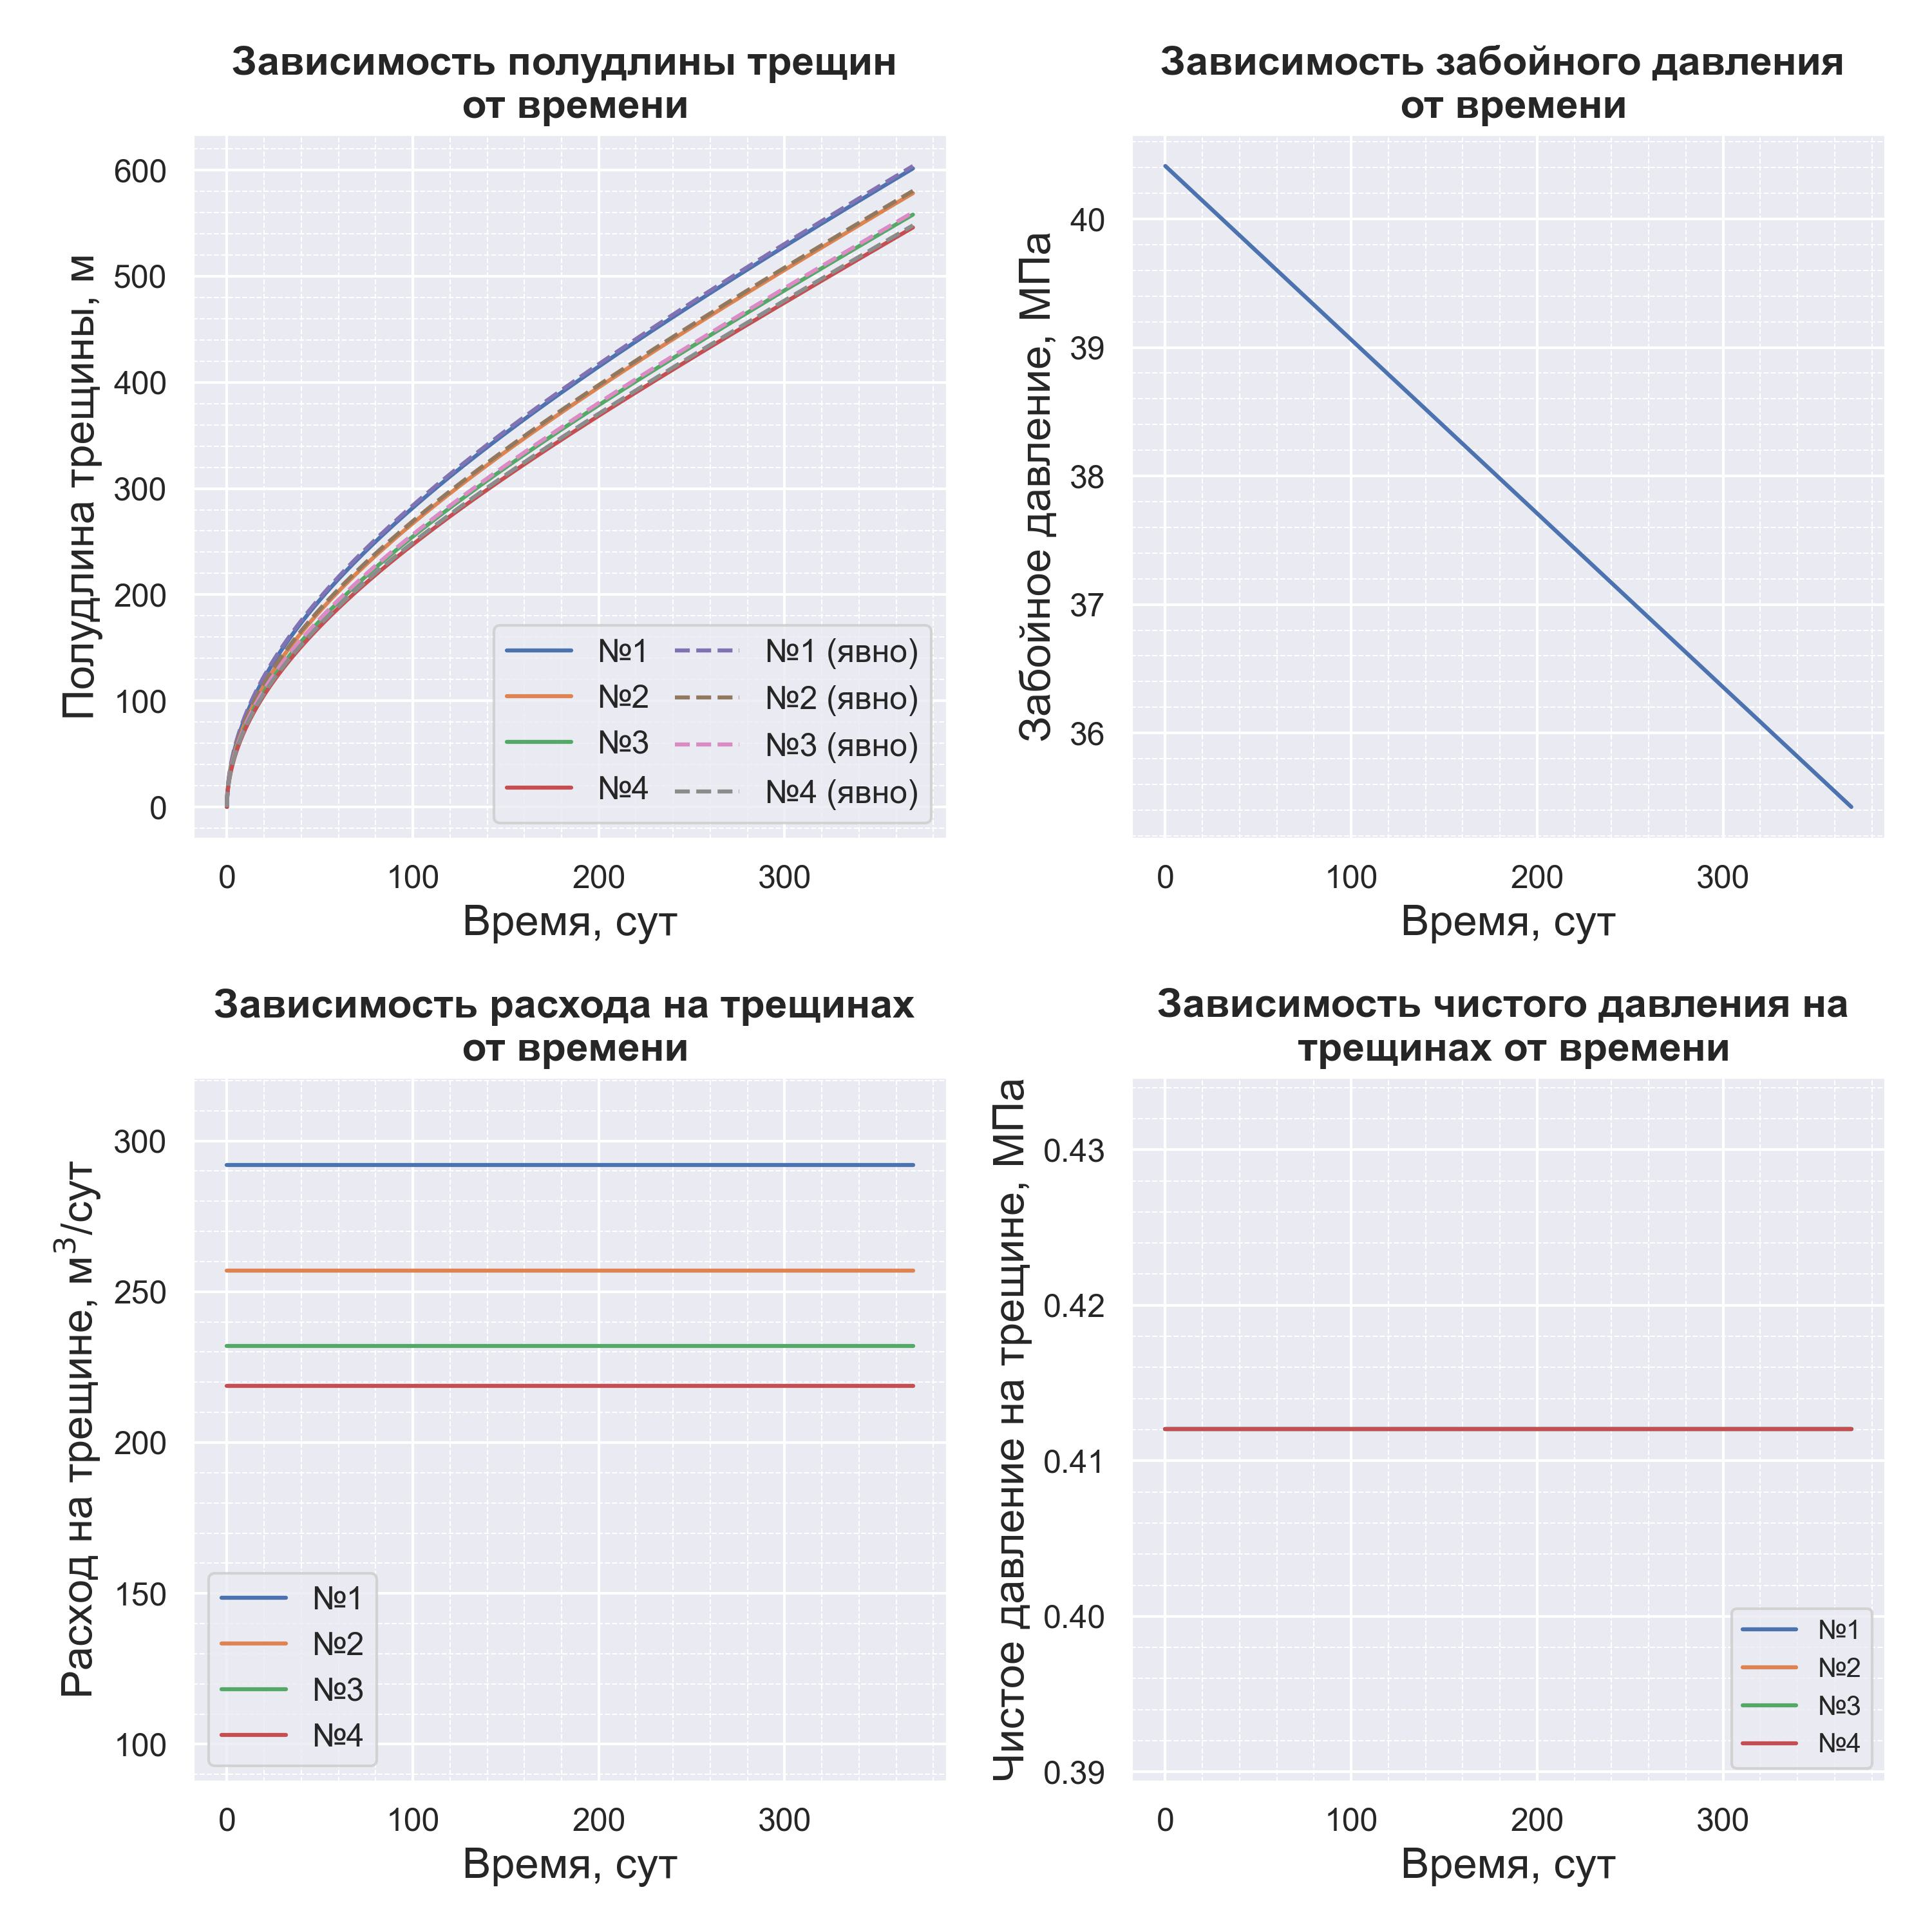
\includegraphics[width=8cm]{myimage12.jpg}}
\end{textblock*}

\end{frame}


\begin{frame}
\frametitle{Результаты при одновременном росте шести трещин}

\begin{textblock*}{8cm}(2.5cm,1.1cm)
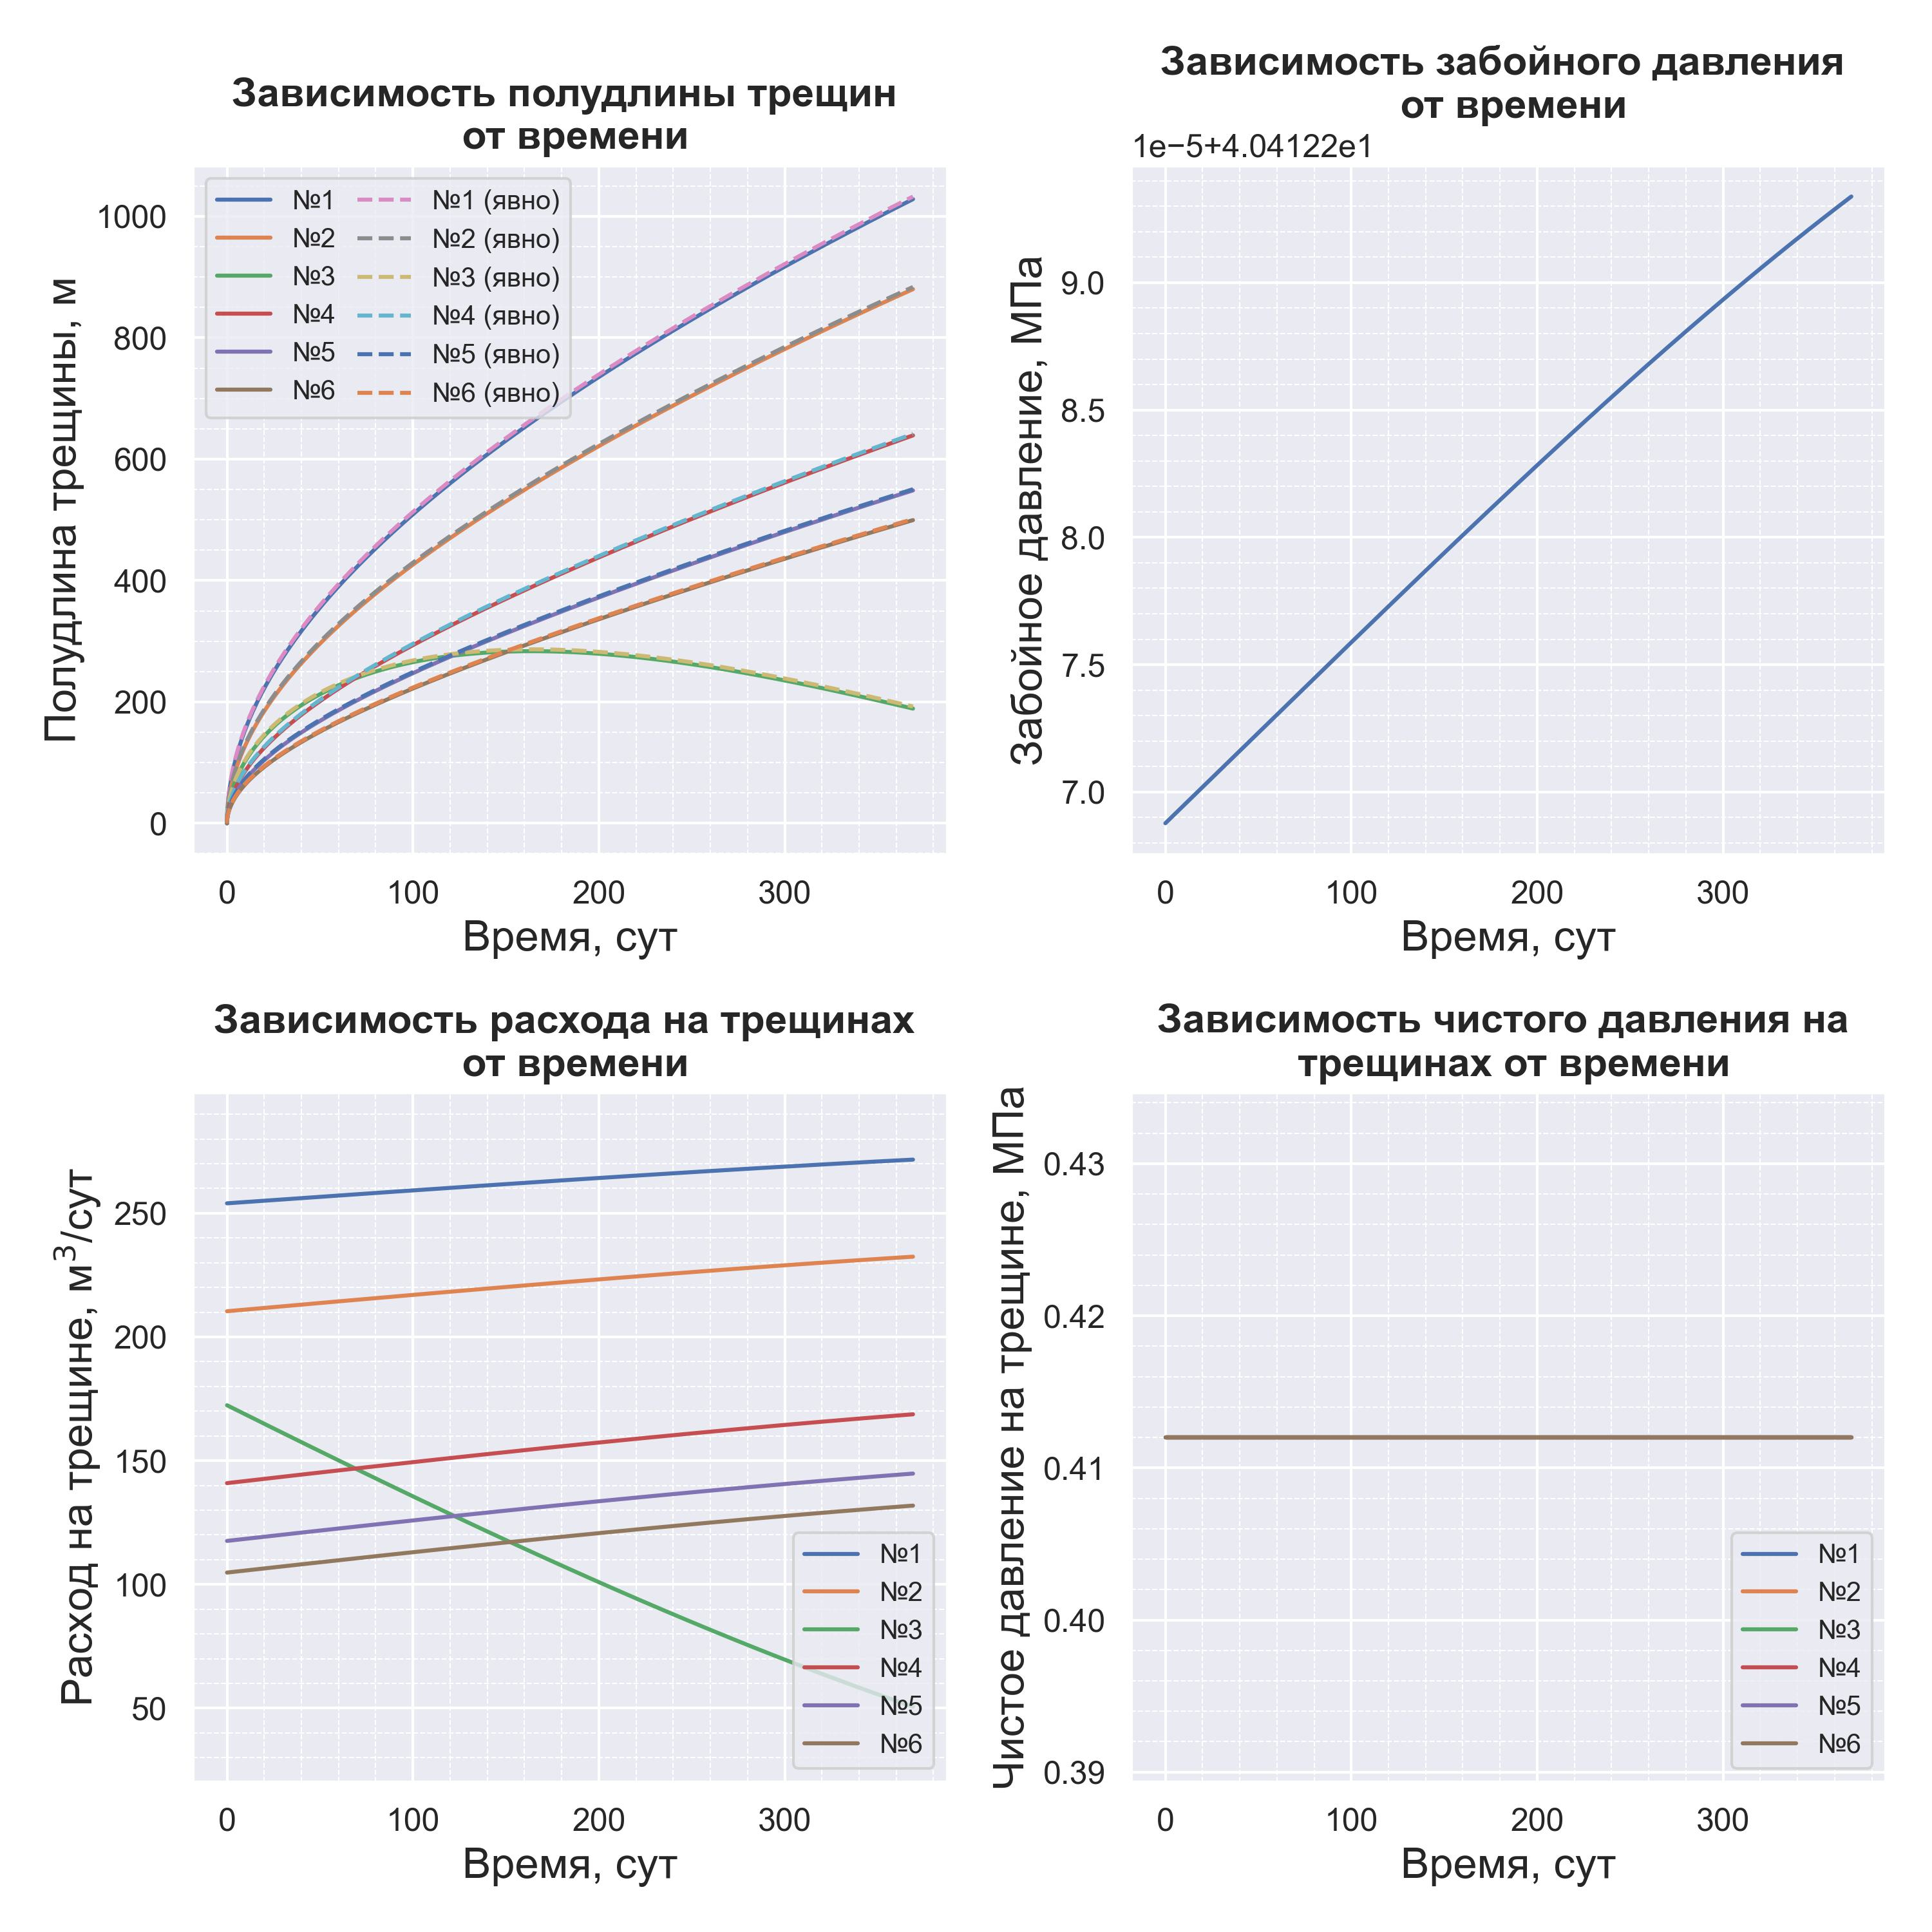
\includegraphics[width=8cm]{myimage13.jpg}
\end{textblock*}

\end{frame}


\begin{frame}
\frametitle{Выводы}

\small
\begin{textblock*}{12cm}(0.3cm,1.1cm)
\begin{itemize}
	\item Реализован численный алгоритм расчёта потоков на каждой из трещин по правилам Кирхгофа (при любом количестве трещин)
	\item Реализован алгоритм расчёта приращения полудлины трещины на каждом шаге по времени с учётом изменяющихся расходов на трещинах (при любом количестве трещин)
	\item Проведён анализ результатов:
	\begin{enumerate}[\large\textbf{--}]
	\item падение давления на трение в трубе приводит к существенной разнице расходов на нескольких трещинах автоГРП и, как следствие, трещина, расположенная близко к забою, растёт более интенсивно 
	\item уменьшение диаметра перфораций на одной из трещин приводит к постепенному закрытию этой трещины и одновременному более интенсивному росту соседних трещин;
	\item уменьшение расхода на забое скважины приводит к уменьшению расходов на трещинах и сокращению их длины;
	\item термоупругое уменьшение горизонтальных напряжений в пласте приводит к более интенсивному росту трещин автоГРП
	\end{enumerate}
\end{itemize}
\end{textblock*}

\normalsize

\end{frame}


\end{document}
